\documentclass[a4paper, 12pt]{scrreprt}
\usepackage[german]{babel}
\usepackage[german]{translator}
\usepackage[utf8]{inputenc}
\usepackage[T1]{fontenc}
\usepackage{ae}
\usepackage[bookmarks,bookmarksnumbered]{hyperref}
\usepackage{graphicx}
\usepackage{color}
\usepackage[dvipsnames]{xcolor}
\usepackage{booktabs}
\usepackage{longtable}
\usepackage{listings}
\usepackage{tabularx}
%\usepackage{pdfpages}
%\usepackage[section]{placeins}


\newcommand{\col}[2]{\textcolor{#1}{#2}}

% Zeilenhöhe bei Tabellen
\newcommand{\zh}[1]{\parbox[0pt][#1][c]{0cm}{}}

\begin{document}
	\thispagestyle{plain}

\begin{titlepage}
    \begin{center}
        \begin{figure}[ht]
            \centering
            
\includegraphics[width=0.66\textwidth, angle=0]{logo/name_blau_ofCourse.jpg}
        \end{figure}

    	\begin{title}
        	\title{\Huge{\textbf{Kurseinheiten-Manager \\ Feinspezifikation\\}}}

		\end{title}
		\hspace{3cm}

        	Software Engineering Praktikum \\
        	Sommersemester 2015\\
        	Universität Passau\\


        	Betreuer: Andreas Stahlbauer \\
        	\hspace{1,5cm}\\
        	Version: 2.0 \\
        	\hspace{1,5cm}\\
        	Datum: 16.05.2015\\[50pt]
        	Team 3 \\
    
		    \ \\
        
        \begin{tabular}{ | l | l | l | l |}
        	\hline
        	\textbf{Matrikelnummer} & \textbf{Name} & \textbf{Phase} & \textbf{E-Mail}  \\ \hline
        	63097 & Katharina Hölzl & Pflichtenheft & hoelzlka@fim.uni-passau.de \\ \hline
        	64504 & Ricky Strohmeier& Entwurf & strohric@fim.uni-passau.de  \\ \hline
        	64380 & Martin Bachhuber & Feinspezifikation  & bachhube@fim.uni-passau.de \\ \hline
        	64080 & Tobias Fuchs & Implementierung  &  fuchstob@fim.uni-passau.de\\ \hline
        	61085 & Sebastian Schwarz & Feinspezifikation & sebastian@nrschwarz.de \\ \hline  
        	58379 & Patrick Cretu  &  Validierung & cretu@fim.uni-passau.de \\ \hline
        \end{tabular}
        
        \ \\
        \ \\
        \hspace{3 cm}\\
         \textbf{Arbeitspakete Feinspezifikation} \\
         \ \\
         
         \begin{tabular}{ | l | l |}
         	\hline
         	\textbf{Autor} & \textbf{Verantwortungsbereich} \\ \hline
         	Katharina Hölzl & View, Javadocs \\ \hline
         	Ricky Strohmeier& View, Javadocs \\ \hline
         	Martin Bachhuber & Paket\"{u}bersicht und Ordner\"{u}bersicht, Security, Sequenzdiagramm, Javadocs  \\ \hline
         	Tobias Fuchs & Klassendiagramm, Javadocs \\ \hline
         	Sebastian Schwarz & Konfigurationsdatei, Klassendiagramm, Javadocs \\ \hline  
         	Patrick Cretu  &  Datenbankschema, Sequenzdiagramm, Javadocs  \\ \hline
         \end{tabular}
        
        
    \end{center}
\end{titlepage}

% Änderungsdokument hinzugefügt
\chapter*{Änderungsübersicht}


% Platzierung des Inhaltsverzeichnisses
\tableofcontents


\chapter{Package\"{u}bersicht und Ordner\"{u}bersicht}

	\newcommand{\class}[1]{\paragraph{Klasse #1:}\ \\ }
	\newcommand{\method}[1]{\textcolor{blue}{#1}}
	\newcommand{\kursiv}[1]{{\it #1}}
	\newcommand{\override}{{\it @Override}\ \\}
	
	\chapter{Klassenbeschreibung und Klassendiagramm}
	In diesem Kapitel werden alle Klassen der Anwendung \textbf{ofCourse} aufgeführt.
	Um eine bessere Übersicht und Strukturierung zu erhalten wird das ganze Projekt in Packages aufgeteilt. Außerdem enthalten folgende Klassen nachfolgende Implementierungen:
	\begin{itemize}
		\item Alle Validator - Klassen: implements Validator
		\item Alle ViewScoped - Klassen: implements Serializable
		\item Alle Exception - Klassen: extends Exception
	\end{itemize}

	\section{Package Action}
		\begin{tiny}
			TF\\
		\end{tiny}\\
	Dieses Package stellt die Businesslogik des Systems \textbf{ofCourse} dar.
	\subsection{Klasse AuthenticateUser}
	\kursiv{ManagedBean, RequestScoped}\\
	Die Klasse ist für die Authentifizierung eines Benutzers im System zuständig.
	\begin{itemize}
		\item \method{public boolean login()}
		\item \method{public User getLoginUser()}
		\item \method{public void setLoginUser(User userToLogIn)}
		\item \method{public SessionUser getSessionUser()}
		\item \method{public void setSessionUser(SessionUser userSession)}
	\end{itemize}
	
	\subsection{Klasse RegisterUser}
	\kursiv{ManagedBean, RequestScoped}\\
	Die Klasse ist für die Registrierung eines Benutzers im System zuständig.
	\begin{itemize}
		\item \method{public boolean registerUser()}
		\item \method{public User getUsertoRegistrate()}
		\item \method{public void setUserToRegistrate(User userToRegistrate)}
		\item \method{public Address getAddress()}
		\item \method{public void setAddress(Address addressToSet)}
		\item \method{public SessionUser getSessionUser()}
		\item \method{public void setSessionUser(SessionUser userSession)}
	\end{itemize}
	
	\subsection{Klasse LostPassword}
	\kursiv{ManagedBean, RequestScoped}\\
	Die Klasse ist für die 'Passwort  vergessen' - Funktion zuständig, d.h. sie ersetzt das alte Passwort eines Benutzers durch ein zufällig generiertes und sendet es an die eingegebene E-Mailadresse.
	\begin{itemize}
		\item \method{public boolean resetPassword()}
		\item \method{public String getEmailAddressToResetPassword()}
		\item \method{public void setEmailAddressToResetPassword(String emailToResetPassword)}
		\item \method{public User getUser()}
		\item \method{public void setUser(User user)}
	\end{itemize}
	
	\subsection{Klasse SearchUser}
	\kursiv{ManagedBean, ViewScoped}\\
	Diese Klasse stellt den Mechanismus zum Suchen von Benutzern zur Verfügung.
	\begin{itemize}
		\item \method{public ArrayList<User> getSearchResult()}
		\item \method{public void setSearchResult(ArrayList<User> searchResult)}
		\item \method{public void search(String searchParam, String searchTerm)}
		\item \method{public String getSearchParam()}
		\item \method{public void setSearchParam(String searchParam)}
		\item \method{public String getSearchTerm()}
		\item \method{public void setSearchTerm(String searchTerm)}
		\item \method{public void sortBySpecificColumn()}
		\item \method{public int getActualPageNumber()}
		\item \method{public void goToSpecificPage()}
		\item \method{public Pagination getPagination()}
		\item \method{public void setPagination(Pagination pagination)}
		\item \method{public SessionUser getSessionUser()}
		\item \method{public void setSessionUser(SessionUser userSession)}
	\end{itemize}
	
	\subsection{Klasse SearchCourse}
	\kursiv{ManagedBean, ViewScoped}\\
	Diese Klasse stellt den Mechanismus zum Suchen von Kursen zur Verfügung. Außerdem wird darin die Einschränkung des angezeigten Kursangebots realisiert.
	\begin{itemize}
		\item \method{public void searchForFreeCourses()}
		\item \method{public void displayCoursesInSpecificPeriod()}
		\item \method{public String getDisplayPeriod()}
		\item \method{public void setDisplayPeriod(String displayPeriod)}
		\item \method{public ArrayList<Course> getSearchResult()}
		\item \method{public void setSearchResult(ArrayList<Course> searchResult)}
		\item \method{public void search(String searchParam, String searchTerm)}
		\item \method{public String getSearchParam()}
		\item \method{public void setSearchParam(String searchParam)}
		\item \method{public String getSearchTerm()}
		\item \method{public void setSearchTerm(String searchTerm)}
		\item \method{public void sortBySpecificColumn()}
		\item \method{public int getActualPageNumber()}
		\item \method{public void goToSpecificPage()}
		\item \method{public Pagination getPagination()}
		\item \method{public void setPagination(Pagination pagination)}
		\item \method{public SessionUser getSessionUser()}
		\item \method{public void setSessionUser(SessionUser userSession)}
	\end{itemize}
	
	\subsection{Klasse UserProfil}
	\kursiv{ManagedBean, ViewScoped}\\
	Diese Klasse ist zuständig für die Anzeige und das Bearbeiten der Benutzerdaten. Des Weiteren realisiert sie die Darstellung der Liste aller vom Benutzer geleiteten Kurse.
	\begin{itemize}
		\item \method{public void editUserdata()}
		\item \method{public void saveUserdata()}
		\item \method{public boolean uploadProfilPic()}
		\item \method{public void setUserInactive()}
		\item \method{public void depositMoneyPerCreditcard()}
		\item \method{public User getUser()}
		\item \method{public void setUser(User userToSet)}
		\item \method{public Address getAddress()}
		\item \method{public void setAddress(Address addressToSet)}
		\item \method{public ArrayList<Course> getManagedCourses()}
		\item \method{public void setManagedCourses(ArrayList<Course> managedCourses)}
		\item \method{public int getActualPageNumber()}
		\item \method{public void goToSpecificPage()}
		\item \method{public Pagination getPagination()}
		\item \method{public void setPagination(Pagination pagination)}
		\item \method{public SessionUser getSessionUser()}
		\item \method{public void setSessionUser(SessionUser userSession)}
	\end{itemize}
	
	\subsection{Klasse CourseDetail}
	\kursiv{ManagedBean, ViewScoped}\\
	Die Klasse ist zuständig für die Anzeige der Kursdetails und das Bearbeiten von Kursen.
	\begin{itemize}
		\item \method{public void editCourse()}
		\item \method{public boolean saveCourse()}
		\item \method{public Course getCourse()}
		\item \method{public void setCourse(Course course)}
		\item \method{public boolean registeredForCourseNews()}
		\item \method{public boolean signUpForCourse() throws CourseRegistrationException}
		\item \method{public boolean signOffForCourse() throws CourseRegistrationException}
		\item \method{public void selectAllCourseUnits()}
		\item \method{public boolean signUpForCourseUnits() throws CourseRegistrationException}
		\item \method{public boolean signOffForCourseUnits() throws CourseRegistrationException}
		\item \method{public ArrayList<CourseUnit> getSelectedCourseUnits()}
		\item \method{public void setSelectedCourseUnits(ArrayList<CourseUnit> selectedCourseUnits)}
		\item \method{public ArrayList<User> getLeadersOfCourse()}
		\item \method{public void setLeadersOfCourse(ArrayList<User> leaders)}
		\item \method{public ArrayList<CourseUnit> getCourseUnitsOfCourse()}
		\item \method{public void setCourseUnitsOfCourse(ArrayList<CourseUnit> courseUnits)}
		\item \method{public String loadParticipientsPage()}
		\item \method{public String loadCreateCourseUnitPage()}
		\item \method{public String loadEditCourseUnitPage()}
		\item \method{public int getActualPageNumber()}
		\item \method{public void goToSpecificPage()}
		\item \method{public Pagination getPagination()}
		\item \method{public void setPagination(Pagination pagination)}
		\item \method{public SessionUser getSessionUser()}
		\item \method{public void setSessionUser(SessionUser userSession)}
	\end{itemize}
	
	\subsection{Klasse CourseUnitManagement}
	\kursiv{ManagedBean, ViewScoped}\\
	Die Klasse ist zuständig für das Anlegen, Bearbeiten und Löschen von Kurseinheiten.
	\begin{itemize}
		 \item \method{public boolean createCourseUnit(boolean isRegular)}
		 \item \method{public void editCourseUnit()}
		 \item \method{public boolean saveCourseUnit(boolean editAllIfRegular)}
		 \item \method{public boolean deleteCourseUnit(boolean deleteAllIfRegular)}
		 \item \method{public boolean addUsersToCourseUnit(ArrayList<User> user)}
		 \item \method{public User getUserToAdd()}
		 \item \method{public void setUserToAdd(User userToAdd)}
		 \item \method{public boolean deleteUserFromCourse()}
		 \item \method{public ArrayList<User> getUserToDelete()}
		 \item \method{public void setUsersToDelete(ArrayList<User> usersToDelete)}
		 \item \method{public boolean getIsRegularCourseUnit()}
		 \item \method{public void setIsRegularCourseUnit(boolean isRegular)}
		 \item \method{public Cycle getCylceOfCourseUnit()}
		 \item \method{public void setCylceOfCourseUnit(Cycle cycle)}
		 \item \method{public CourseUnit getCourseUnit()}
		 \item \method{public void setCourseUnit(CourseUnit courseUnit)}
		 \item \method{public Address getAddress()}
		 \item \method{public void setAddress(Address addressToSet)}
		 \item \method{public ArrayList<User> getParticipientsOfCourseUnit()}
	  	 \item \method{public void setParticipientsOfCourseUnit(ArrayList<User> participients)}
		 \item \method{public int getActualPageNumber()}
		 \item \method{public void goToSpecificPage()}
		 \item \method{public Pagination getPagination()}
		 \item \method{public void setPagination(Pagination pagination)}
		 \item \method{public SessionUser getSessionUser()}
		 \item \method{public void setSessionUser(SessionUser userSession)}
	\end{itemize}
	
	\subsection{Klasse ContactUsers}
	\kursiv{ManagedBean, RequestScoped}\\
	Die Klasse ist zuständig für die Benachrichtigung von Benutzern durch Kursleiter oder Administratoren.
	\begin{itemize}
		\item \method{public boolean sendEMail() throws MailingException}
		\item \method{public Mail getMail()}
	    \item \method{public void setMail(Mail mail)}
		\item \method{public String getSubject()}
		\item \method{public void setSubject(String subject)}
	    \item \method{public String getMessageToSend()}
	    \item \method{public void setMessageToSend(String messageToSend)}
		\item \method{public ArrayList<String> getMailRecipients()}
		\item \method{public void setMailRecipients(ArrayList<String> mailRecipients)}
        \item \method{public SessionUser getSessionUser()}
        \item \method{public void setSessionUser(SessionUser userSession)}
	\end{itemize}
	
	\subsection{Klasse MyCourses}
	\kursiv{ManagedBean, RequestScoped}\\
	Die Klasse ist zuständig für die Anzeige der angemeldeten Kurse eines Benutzers.
	\begin{itemize}
		\item \method{public ArrayList<Course> getRegisteredCourses()}
		\item \method{public void setRegisteredCourses(ArrayList<Course> registeredCourses)}
		\item \method{public String loadCourseDetailsPageOfSelectedCourse()}
		\item \method{public int getActualPageNumber()}
		\item \method{public void goToSpecificPage()}
		\item \method{public Pagination getPagination()}
		\item \method{public void setPagination(Pagination pagination)}
		\item \method{public SessionUser getSessionUser()}
		\item \method{public void setSessionUser(SessionUser userSession)}
	\end{itemize}
	
	\subsection{Klasse CourseManagement}
	\kursiv{ManagedBean, ViewScoped}\\
	Die Klasse ist zuständig für die Verwaltung der Kurse, d.h. für das Anlegen und Löschen von Kursen sowie die Trainerverwaltung.
	\begin{itemize}
		\item \method{public boolean createCourse(Course course)}
		\item \method{public boolean uploadCoursePic()}
		\item \method{public boolean deleteCourse()}
		\item \method{public boolean addCourseLeader(User leader)}
		\item \method{public User getLeaderToAdd()}
		\item \method{public void setLeaderToAdd(User leaderToAdd)}
		\item \method{public boolean removeCourseLeader()}
		\item \method{public boolean removeCourseLeaders()}
		\item \method{public ArrayList<User> getLeadersToDelete()}
		\item \method{public void setLeadersToDelete(ArrayList<User> leadersToDelete)}
		\item \method{public User getCourseLeader()}
		\item \method{public void setCourseLeader()}
		\item \method{public Course getCourse()}
		\item \method{public void setCourse(Course course)}
		\item \method{public Address getAddress()}
		\item \method{public void setAddress(Address address)}
		\item \method{public SessionUser getSessionUser()}
		\item \method{public void setSessionUser(SessionUser userSession)}
	\end{itemize}
	
	\subsection{Klasse AccountManagment}
	\kursiv{ManagedBean, RequestScoped}\\
	Die Klasse ist für die Aktivierung von Benutzeraccounts durch einen Kursleiter oder Administrator zuständig.
	\begin{itemize}
		\item \method{public boolean activateAccounts()}
		\item \method{public ArrayList<User> getUsersToActivate()}
		\item \method{public void setUsersToActivate(ArrayList<User> usersToActivate)}
		\item \method{public ArrayList<User> getSelectedUsers()}
		\item \method{public void setSelectedUsers(ArrayList<User> selectedUsers)}
		\item \method{public int getActualPageNumber()}
		\item \method{public void goToSpecificPage()}
		\item \method{public Pagination getPagination()}
		\item \method{public void setPagination(Pagination pagination)}
		\item \method{public SessionUser getSessionUser()}
		\item \method{public void setSessionUser(SessionUser userSession)}
	\end{itemize}	
	
	\subsection{Klasse UserManagement}
	\kursiv{ManagedBean, ViewScoped}\\
	Die Klasse ist zuständig für die Benutzerverwaltung, d.h. das Anlegen von Benutzern und das Löschen von Benutzern.
	\begin{itemize}
		\item \method{public boolean createUser(User user)}
		\item \method{public boolean uploadProfilPic()}
		\item \method{public boolean deleteUser()}
		\item \method{public User getUser()}
		\item \method{public void setUser(User user)}
		\item \method{public Address getAddress()}
		\item \method{public void setAddress(Address address)}
		\item \method{public SessionUser getSessionUser()}
		\item \method{public void setSessionUser(SessionUser userSession)}
	\end{itemize}
	
	\subsection{Klasse ListParticipents}
	\kursiv{ManagedBean, RequestScoped}\\
	Die Klasse ist zuständig für das Anzeigen der Teilnehmer einer Kurseinheit oder eines Kurses und für die Entfernung einzelner Benutzer aus Kursen oder Kurseinheiten.
	\begin{itemize}
		\item \method{public ArrayList<User> getParticipients()}
		\item \method{public void setParticipients(ArrayList<User> participients)}
		\item \method{public boolean deleteUserFromCourse()}
		\item \method{public ArrayList<User> getUserToDelete()}
		\item \method{public void setUsersToDelete( ArrayList<User> usersToDelete)}
		\item \method{public int getActualPageNumber()}
		\item \method{public void goToSpecificPage()}
		\item \method{public Pagination getPagination()}
		\item \method{public void setPagination(Pagination pagination)}
		\item \method{public SessionUser getSessionUser()}
		\item \method{public void setSessionUser(SessionUser userSession)}
	\end{itemize}
	
	\subsection{Klasse SystemConfiguration}
	\kursiv{ManagedBean, ViewScoped}\\
	Die Klasse ist für Einstellungen bezüglich des Systems zuständig, d.h. das Hochladen einer CSS - Datei, eines Logos, des Festlegen des Überziehungskredits und der Registrierungseinstellungen. Des Weiteren ist sie zuständig für die Weiterleitung zur Benutzer- und Kursverwaltung.
	\begin{itemize}
		\item \method{public void determineAccountActivationType(String accountActivationType)}
		\item \method{public String getAccountActivationType()}
		\item \method{public void setAccountActivationType(String accountActivationType)}
		\item \method{public void determineOverdraftCredit(float overdraftCredit)}
		\item \method{public float getOverdraftCredit()}
		\item \method{public void setOverdraftCredit(float overdraftCredit)}
		\item \method{public boolean uploadCustomStyleCSS()}
		\item \method{public boolean uploadLogo()}
		\item \method{public String loadEditImprintPage()}
		\item \method{public String loadCreateNewUserPage()}
		\item \method{public String loadManageUserPage()}
		\item \method{public String loadCreateNewCoursePage()}
		\item \method{public String loadManageCoursesPage()}
		\item \method{public System getSystem()}
		\item \method{public void setSystem(System system)}
		\item \method{public SessionUser getSessionUser()}
		\item \method{public void setSessionUser(SessionUser userSession)}
	\end{itemize}
	
	\subsection{Klasse PaymentOnline}
	\kursiv{ManagedBean, ViewScoped}\\
	Die Klasse ist zuständig für die Online - Aufladung des Guthabenkontos von Benutzern per Kreditkarte. Die Kreditkartenabwicklung erfolgt über die InfoSun-Bank.
	\begin{itemize}
		\item \method{public boolean depositAmount() throws BankAccountException}
		\item \method{public User getUser()}
		\item \method{public void setUser(User user)}
	    \item \method{public PaymentInformation getPaymentInformation()}
	    \item \method{public void setPaymentInformation(PaymentInformation payInfo)}
		\item \method{public SessionUser getSessionUser()}
		\item \method{public void setSessionUser(SessionUser userSession)}
	\end{itemize}
	
	\subsection{Klasse PaymentOffline}
	\kursiv{ManagedBean, ViewScoped}\\
	Die Klasse ist zuständig für die Offline - Aufladung des Guthabenkontos von Benutzern durch den Administrator und um die Bezahlungseinstellungen zu verwalten.
	\begin{itemize}
		\item \method{public boolean depositAmountOnUserAccount() throws BankAccountException}
		\item \method{public User getUser()}
		\item \method{public void setUser(User user)}
		\item \method{public int getAmountToDeposit()}
		\item \method{public void setAmountToDeposit(float amountToDeposit)}
		\item \method{public SessionUser getSessionUser()}
		\item \method{public void setSessionUser(SessionUser userSession)}
	\end{itemize}
	
	\subsection{Klasse IncomeStatistics}
	\kursiv{ManagedBean, RequestScoped}\\
	Die Klasse ist für die Generierung und Darstellung der Einnahmestatistiken zuständig.
	\begin{itemize}
	    \item \method{public void displayStatistic(String displayParam)}
		\item \method{public String getDisplayParam()}
		\item \method{public void setDisplayParam(String displayParam)}
		\item \method{public int getActualPageNumber()}
		\item \method{public void goToSpecificPage()}
		\item \method{public Pagination getPagination()}
		\item \method{public void setPagination(Pagination pagination)}
		\item \method{public SessionUser getSessionUser()}
		\item \method{public void setSessionUser(SessionUser userSession)}
	\end{itemize}
	
	\subsection{Klasse EditImprint}
	\kursiv{ManagedBean, ViewScoped}\\
	Die Klasse ist für die Darstellung und Bearbeitung des Impressums verantwortlich.
	\begin{itemize}
		\item \method{public void editImprint(String imprint)}
		\item \method{public String getImprint()}
		\item \method{public void setImprint(String imprint)}
		\item \method{public SessionUser getSessionUser()}
		\item \method{public void setSessionUser(SessionUser userSession)}
	\end{itemize}
	
	\subsection{Klasse Header}
	\kursiv{ManagedBean, RequestScoped}\\
	Diese Klasse ist zuständig für das Laden der Anmeldeseite, das Abmelden und der Auswahl der Anzeigesprache.
	\begin{itemize}
		\item \method{public String login()}
		\item \method{public boolean logout()}
		\item \method{public String getChoosenLanguage()}
		\item \method{public void setChoosenLanguage(String choosenLanguage)}
		\item \method{public SessionUser getSessionUser()}
		\item \method{public void setSessionUser(SessionUser userSession)}
	\end{itemize}
	
	\subsection{Klasse Footer}
	\kursiv{ManagedBean, RequestScoped}\\
	Diese Klasse ist zuständig für das Laden der AGB, der Hilfe und der Impressumsseite.
	\begin{itemize}
		\item \method{public String loadImprintPage()}
		\item \method{public String loadAGBPage()}
		\item \method{public String loadHelpPage()}
	\end{itemize}
	
	\subsection{Klasse Scheduler}
	\kursiv{ManagedBean, RequestScoped}\\
	Diese Klasse ist zuständig für die Generierung und Darstellung des persönlichen Terminplaners des Benutzers.
	\begin{itemize}
		\item \method{public void displayScheduler(ArrayList<CourseUnit> bookedCourseUnits)}
		\item \method{public void displayNextWeek()}
		\item \method{public void displayPreviousWeek()}
		\item \method{public SessionUser getSessionUser()}
		\item \method{public void setSessionUser(SessionUser userSession)}
	\end{itemize}
	
	\subsection{Klasse SessionUser}
	\kursiv{ManagedBean, SessionScoped}\\
	Die Klasse speichert Informationen über die Session eines Benutzers. Gespeichert werden die ID des Benutzers, dessen Benutzerrolle, der aktuelle Status des Benutzers und die gewählte Sprache.
	\begin{itemize}
		\item \method{public int getUserID()}
		\item \method{public void setUserID(int userID)}
		\item \method{public int getUserStatus()}
		\item \method{public void setUserStatus(int userStatus)}
		\item \method{public String getUserRole()}
		\item \method{public void setUserRole(String userRole)}
		\item \method{public String getLanguage()}
		\item \method{public void setLanguage(String language)}
	\end{itemize}
	
	\subsection{Klasse Mail}
	\kursiv{ManagedBean, ApplicationScoped}\\
	Die Klasse ist für die E-Mailbenachrichtigung der Benutzer zuständig. Sie ist sowohl für die automatisch gesendeten E-Mails, wie unter anderem die Verifizierung oder Accountaktivierungsbestätigung, als auch für die von Kursleitern gesendeten Mails zuständig.
	\begin{itemize}
		\item \method{public boolean sendVerificationMail(int UserID) throws MailingException}
		\item \method{public boolean sendConfirmaitionMail(int UserID) throws MailingException}
		\item \method{public boolean sendMail(String subject, String message, ArrayList<String> mailRecipients) throws MailingException}
		\item \method{public SmtpServer getSmtpServer()}
		\item \method{public void setSmtpServer(SmtpServer smtpServer)}
	\end{itemize}
	
	\section{Package Model}
	\begin{tiny}
		SeSc \\
	\end{tiny}\\
	Das Pakte Model enthält die Klassen für Aufzählungstypen. Die privaten Attribute können durch die jeweiligen \glqq getter\grqq- \ und \glqq setter\grqq- \ Methoden aufgerufen und gesetzt werden.
	\subsection{Klasse SmtpServer}
	Die Klasse enthält die Zugangsdaten des E-Mail Servers.
	\begin{itemize}
		\item \method {public String getHostaddr()}
		\item \method {public String getPassword()}
		\item \method {public int getPort()}
		\item \method {public String getUsername()}
		\item \method {public boolean isAuthentificated()}
		\item \method {public boolean isTls()}
		\item \method {public void setAuthentificated(Boolean authentificated)}
		\item \method {public void setHostaddr(String hostaddr)}
		\item \method {public void setPassword(String password)}
		\item \method {public void setPort(int port)}
		\item \method {public void setTls(Boolean tls)}
		\item \method {public void setUsername(String username)}
	
	\end{itemize}
	
	\subsection{Klasse Pagination}
	Die Klasse steuert die Anzeige von Listen der Kurse, Benutzer und Benutzereinheiten um Skalierbarkeit zu bewahren.
	\begin{itemize}
		\item \method {public int getItemsPerPage()}
		\item \method {public int getShownPageNum()}
		\item \method {public String getSortColumn()}
		\item \method {public boolean isSortAsc()}
		\item \method {public void setItemsPerPage(int itemsPerPage)}
		\item \method {public void setSortColumn(String sortColumn)}
		\item \method {public void setShownPageNum(int shownPageNum)}
		\item \method {public void setSortAsc(boolean sortAsc)}
	\end{itemize}
	
	\subsection{Klasse Course}
	\begin{itemize}
		\item \method {public String getTitle()}
		\item \method {public String getDiscription()}
		\item \method {public CourseUnit getNextCourseUnit()}
		\item \method {public Date getStartdate()}
		\item \method {public Date getEnddate()}
		\item \method {public int getMaxUsers()}
		\item \method {public ArrayList<CourseUnit> getCourseUnits()}
		\item \method {public ArrayList<User> getCoursAdmins()}
		\item \method {public ArrayList<User> getUsers()}
		\item \method {public ArrayList<User> getUsersToInform()}
		\item \method {public void setTitle(String title)}
		\item \method {public void setDiscription(String discription)}
		\item \method {public void setNextCourseUnit(CourseUnit nextCourseUnit)}
		\item \method {public void setStartdate(Date startDate)}
		\item \method {public void setEnddate(Date endDate)}
		\item \method {public void setMaxUsers(int maxUsers)}
		\item \method {public void setCourseUnits(ArrayList<CourseUnit> courseUnits) }
		\item \method {public void setCourseAdmins(ArrayList<User> coursAdmins)}
		\item \method {public void setUsers(ArrayList<User> users)}
		\item \method {public void setUsersToInform(ArrayList<User> usersToInform)}  
	\end{itemize}
	
	
	\subsection{Klasse CourseUnit}
	\begin{itemize}
		\item \method {public String getTitle()}
		\item \method {public String getDiscription()}
		\item \method {public Date getStarttime()}
		\item \method {public Date getEndtime()}
		\item \method {public Address getAddress()}
		\item \method {public float getPrice()}
		\item \method {public int getMaxUsers()}
		\item \method {public int getMinUsers()}
		\item \method {public User getCourseAdmin()}
		\item \method {public ArrayList<User> getUsers()}
		\item \method {public void setTitle(String title)}
		\item \method {public void setDiscription(String discription)}
		\item \method {public void setStarttime(Date startingTime)}
		\item \method {public void setEndtime(Date endTime)}
		\item \method {public void setAddress(Address address)}
		\item \method {public void setPrice(float price)}
		\item \method {public void setMaxUsers(int maxUsers)}
		\item \method {public void setMinUsers(int minUsers)}
		\item \method {public void setCourseAdmin(User courseAdmin)}
		\item \method {public void setUsers(ArrayList<User> users)} 
		\end{itemize}
	
	
	\subsection{Klasse User}
	Diese Klasse stellt alle Benutzer des Systems dar. Je nach Status des Benutzers(Administrator, Kursleiter und Benutzer) sind unterschiedliche Attribute ausgefüllt.
	\begin{itemize}
		\item \method {public Address getAddress()}
		\item \method {public boolean equals(Object other)}
		\item \method {public String getEmail()}
		\item \method {public String getFristname()}
		\item \method {public String getLastname()}
		\item \method {public String getUsernname()}
		\item \method {public String getPassword()}
		\item \method {public Date getDateOfBirth()}
		\item \method {public UserRole getUserRole()}
		\item \method {public int getUserID()}
		\item \method {public int hashCode()}
		\item \method {public void setAddress(Address address)}
		\item \method {public void setEmail(String email)}
		\item \method {public void setFirstname(String firstname)}
		\item \method {public void setLastname(String lastname)}
		\item \method {public void setPassword(String password)}
		\item \method {public void setUserRole(UserRole role)}
		\item \method {public void setUserId(int id)}
		\item \method {public void setUsername(String username)}
		\item \method {public void setDateOfBirth(Date dateOfBirth)}
	\end{itemize}
	\subsection{Enumeration UserRole}
	Es werden nun die verschiedenen Benutzerrollen beschrieben.
	\begin{itemize}
		\item {REGISTERED\_USER}
		\item {COURSE\_LEADER}
		\item {SYSTEM\_ADMINISTRATOR}
	\end{itemize}
	
	\subsection{Enumeration UserStatus}
	Es werden nun die verschiedenen Statuszustände eines Benutzers beschrieben.
	\begin{itemize}
		\item {ANONYMOUS}
		\item {NOT\_ACTIVATED}
		\item {REGISTERED}
		\item {INACTIVE}
	\end{itemize}

	
	\subsection{Klasse Address}
	Diese Klasse verwaltet die Adressenangaben der Kurseinheiten und Benutzer.
	\begin{itemize}
		\item \method {public boolean equals(Object other)}
		\item \method {public String getCountry()}
		\item \method {public String getTown()}
		\item \method {public String getStreet()}
		\item \method {public String getRoom()}
		\item \method {public int getHouseNumber()}
		\item \method {public int getZipCode()}
		\item \method {public void setCountry(String country)}
		\item \method {public void setTown(String town)}
		\item \method {public void setStreet(String street)}
		\item \method {public void setRoom(String room)}
		\item \method {public void setHouseNumber(int houseNumber)}
		\item \method {public void setZipCode(int zipCode)}
		
	\end{itemize}
	
	\subsection{Klasse PaymentInformation}
	Diese Klasse stellt die Kreditkarteninformationen, Bankdaten und den Einzahlungsbetrag
	dar.
	\begin{itemize}
		\item \method{public String getAccountNumber()}
		\item \method{ public void setAccountNumber(String accountNumber)}
		\item \method{public int getAmount()}
		\item \method{ public void setAmount(int amount)}
		\item \method{public String getCcHolder()}
		\item \method{ public void setCcHolder(String ccHolder)}
		\item \method{ public String getCcNumber()}
		\item \method{ public void setCcNumber(String ccNumber)}
		\item \method{ public Date getCcValidFrom()}
		\item \method{ public void setCcValidFrom(Date ccValidFrom)}
		\item \method{ public Date getCcValidTo()}
		\item \method{ public void setCcValidTo(Date ccValidTo)}
		\item \method{ public int getCvc()}
		\item \method{ public void setCvc(int cvc)}
		
	\end{itemize}
	
	\subsection{Klasse System}
	In dieser Klasse werden die editierbaren Eigenschaften des Systems gespeichert.
	\begin{itemize}
		\item \method {public boolean equals(Object other)}
		\item \method {public String getCSS()}
		\item \method {public String getImpressum()}
		\item \method {public String getLogo()}
		\item \method {public String getTitle()}
		\item \method {public void setCss(String css)}
		\item \method {public void setImpressum (String impressum)}
		\item \method {public void setLogo(String logo)}
		\item \method {public void setTitle(String title)}
	\end{itemize}
	
	\section{Package Services}
	\begin{tiny}
		TF
	\end{tiny}
    \subsection{Klasse HttpsHelper}
    Dies ist eine Hilfsklasse für Https-Verbindungen.
    \begin{itemize}
    	\item \method{public static void setup()}
    \end{itemize}
    
    \subsection{Klasse TransferAction}
    Diese Klasse übermittelt die Zahlungsdaten an die Bank und liefert eine Zahlungsbestätigung
    zurück.
	    \begin{itemize}
	    	\item \method{public static boolean executeBankTransaktion(PaymentInformation payInfo)}
	    \end{itemize}
    
	\section{Package Interfaces}
	\begin{tiny}
		TF\\
	\end{tiny}\\
	Dieses Package stellt Interfaces zur Verfügung, welche die DAO - Klassen implementieren müssen damit gegebenenfalls  ein Wechsel der Datenbank einfach möglich ist.
	    \class{UserInteraction}
		Dieses Interface gibt vor, welche Methoden für Datenbankanfragen für das Erhalten bzw. das Schreiben von Benutzerdaten vorhanden sein müssen.
		\begin{itemize}
			\item \method{public boolean createUser(User user, Address address)}
			\item \method{public ArrayList<User> getUsers(Pagination pagination)}
			\item \method{public ArrayList<User> getUsers(Pagination pagination, String searchString)}
			\item \method{public ArrayList<User> getUsersOrdered(Pagination pagination, String searchString, String orderParam)}
			\item \method{public User getUser(int userID)}
			\item \method{public int getUserID(String username)}
			\item \method{public boolean updateUser(User user, Address address)}
			\item \method{public boolean deleteUser(int userID)}
			\item \method{public ArrayList<Course> getCoursesLeadedBy(int userID, Pagination pagination)}
		\end{itemize}
		
		\class{CourseInteraction}
		Dieses Interface gibt vor, welche Methoden für Datenbankanfragen für das Erhalten bzw. das Schreiben von Kursdaten vorhanden sein müssen.
		\begin{itemize}
			\item \method{public boolean createCourse(Course course, Address address)}
			\item \method{public ArrayList<Course> getCourses(Pagination pagination)}
			\item \method{public ArrayList<Course> getCourses(Pagination pagination, String searchString)}
			\item \method{public ArrayList<Course> getCoursesOrdered(Pagination pagination, String searchString, String orderParam)}
			\item \method{public ArrayList<User> getLeaders(int courseID)}
			\item \method{public Course getCourse(int courseID)}
			\item \method{public boolean updateCourse(Course course, Address address)}
			\item \method{public boolean deleteCourse(int courseID)}
			\item \method{public boolean addUserToCourse(int userID)}
			\item \method{public boolean removeUserFromCourse(int userID)}
			\item \method{public boolean addLeaderToCourse(int userID)}
			\item \method{public boolean removeLeaderFromCourse(int userID)}
		\end{itemize}
		
		\class{CourseUnitInteraction}
			Dieses Interface gibt vor, welche Methoden für Datenbankanfragen für das Erhalten bzw. das Schreiben von Kurseinheitsdaten vorhanden sein müssen.
		\begin{itemize}
			\item \method{public boolean createCourseUnit(CourseUnit courseUnit, Address address)}
			\item \method{public CourseUnit getCourseUnit(int courseUnitID)}
			\item \method{public ArrayList<CourseUnit> getCourseUnitsFromCourse(int courseID, Pagination pagination)}
			\item \method{public boolean updateCourseUnit(CourseUnit courseUnit, Address address)}
			\item \method{public boolean deleteCourseUnit(int courseUnitID)}
			\item \method{public boolean addUserToCourseUnit(int userID)}
			\item \method{public boolean removeUserFromCourseUnit(int userID)}
		\end{itemize}
		
		\class{StatisticsInteraction}
			Dieses Interface gibt vor, welche Methoden für Datenbankanfragen für das Erhalten von Statistikdaten oder das Schreiben dieser in die Datenbank vorhanden sein müssen.
			\begin{itemize}
				\item \method{public HashMap<Date, Float> getIncomePerDay(Date actualDate)}
				\item \method{public HashMap<Date, Float> getIncomePerWeek(Date actualDate)}
				\item \method{public HashMap<User, Float> getIncomePerLeader(Pagination pagination)}
				\item \method{public HashMap<Course, Float> getIncomePerCourse(Pagination pagination)}
			\end{itemize}
		
	\section{Package Database}
	\begin{tiny}
		TF
	\end{tiny}
	\subsection{Package DatabaseGeneral}
	
		\class{SetupAdmin}
		Diese Klasse ist zuständig für das Erstellen des ersten Systemadministrators.
		\begin{itemize}
			\item \method{public boolean createInitialAdmin()}
			\item \method{public boolean createDefaultImprint()}
		\end{itemize}
	
		\class{DatabaseTableCreator}
		Diese Klasse ist zuständig für das Erstellen der Tabellen in der Datenbank, falls diese noch nicht existieren.
		\begin{itemize}
			\item \method{public static boolean buildUpDatabase() throws InvalidDatabaseTransferException}
		\end{itemize}
	
		\class{DatabaseTableDetroyer}
		Diese Klasse ist zuständig für das Löschen der Tabellen in der Datenbank, falls diese existieren.
		\begin{itemize}
			\item \method{public static boolean destroyDatabaseTables() throws InvalidDatabaseTransferException}
		\end{itemize}
	
	\subsection{Package DAO}
		\class{UserDAO}
		Diese Klasse stellt Datenbankanfragen zur Verfügung um Benutzerdaten zu erhalten oder in die
		Datenbank zu schreiben.\\
		Sämtliche Methoden können die \kursiv{InvalidDatabaseTransferException} werfen.
		\begin{itemize}
			\item \method{public boolean createUser(User user, Address address)}
			\item \method{public ArrayList<User> getUsers(Pagination pagination)}
			\item \method{public ArrayList<User> getUsers(Pagination pagination, String searchString)}
			\item \method{public ArrayList<User> getUsersOrdered(Pagination pagination, String searchString, String orderParam)}
			\item \method{public User getUser(int userID)}
			\item \method{public int getUserID(String username)}
			\item \method{public boolean updateUser(User user, Address address)}
			\item \method{public boolean deleteUser(int userID)}
			\item \method{public ArrayList<Course> getCoursesLeadedBy(int userID, Pagination pagination)}
			\end{itemize}
		
		\class{CourseDAO}
		Diese Klasse stellt Datenbankanfragen zur Verfügung um Kursdaten zu erhalten oder in die Datenbank
		zu schreiben.\\
		Sämtliche Methoden können die \kursiv{InvalidDatabaseTransferException} werfen.
		\begin{itemize}
			\item \method{public boolean createCourse(Course course, Address address)}
			\item \method{public ArrayList<Course> getCourses(Pagination pagination)}
			\item \method{public ArrayList<Course> getCourses(Pagination pagination, String searchString)}
			\item \method{public ArrayList<Course> getCoursesOrdered(Pagination pagination, String searchString, String orderParam)}
			\item \method{public ArrayList<User> getLeaders(int courseID)}
			\item \method{public Course getCourse(int courseID)}
			\item \method{public boolean updateCourse(Course course, Address address)}
			\item \method{public boolean deleteCourse(int courseID)}
			\item \method{public boolean addUserToCourse(int userID)}
			\item \method{public boolean removeUserFromCourse(int userID)}
			\item \method{public boolean addLeaderToCourse(int userID)}
			\item \method{public boolean removeLeaderFromCourse(int userID)}
		\end{itemize}
		
		\class{CourseUnitDAO}
		Diese Klasse stellt Datenbankanfragen zur Verfügung um Kurseinheitsdaten zu erhalten oder in die Datenbank zu schreiben.\\
		Sämtliche Methoden können die \kursiv{InvalidDatabaseTransferException} werfen.
		\begin{itemize}
			\item \method{public boolean createCourseUnit(CourseUnit courseUnit, Address address)}
			\item \method{public CourseUnit getCourseUnit(int courseUnitID)}
			\item \method{public ArrayList<CourseUnit> getCourseUnitsFromCourse(int courseID, Pagination pagination)}
			\item \method{public boolean updateCourseUnit(CourseUnit courseUnit, Address address)}
			\item \method{public boolean deleteCourseUnit(int courseUnitID)}
			\item \method{public boolean addUserToCourseUnit(int userID)}
			\item \method{public boolean removeUserFromCourseUnit(int userID)}
		\end{itemize}
		
		\class{StatisticDAO}
		Diese Klasse stellt Datenbankanfragen zur Verfügung um Statistikdaten zu erhalten oder in die Datenbank
		zu schreiben.\\
		Sämtliche Methoden können die \kursiv{InvalidDatabaseTransferException} werfen.
		\begin{itemize}
			\item \method{public HashMap<Date, Float> getIncomePerDay(Date actualDate)}
			\item \method{public HashMap<Date, Float> getIncomePerWeek(Date actualDate)}
			\item \method{public HashMap<User, Float> getIncomePerLeader(Pagination pagination)}
			\item \method{public HashMap<Course, Float> getIncomePerCourse(Pagination pagination)}
		\end{itemize}
	
	\section{Package System}
	\begin{tiny}
		TF
	\end{tiny}
	\subsection{Klasse CheckPhase}
	Die Klasse ist zuständig für die Überprüfung, ob der jeweilige Benutzer die Berechtigung besitzt, auf die angeforderte Seite zu gelangen.\\
	Die Klasse implementiert das Interface PhaseListener.
	\begin{itemize}
		\item \method{public PhaseId getPhaseId()}
		\item \override
		\method{public void beforePhase(PhaseEvent arg0)}
		\item \override
		\method{public void afterPhase(PhaseEvent event)}	
	\end{itemize}
	
	\subsection{Klasse Maintenance}
	Die Klasse ist zuständig den Wartungsthread, der dafür sorgt, dass Kurse sechs Monate nach ihrem Enddatum automatisch aus dem System gelöscht werden.\\
	Die Klasse implementiert das Interface Runnable.
	\begin{itemize}
		\item \method{public boolean isMaintenaceStopped()}
		\item \method{public synchronized void shutDown()}
		\item \method{public static Maintenance getInstance()}
		\item \override
		\method{public void run()}
	\end{itemize}
	
	\subsection{Klasse LaunchSystem}
	\kursiv{ManagedBean, ApplicationScoped}\\
	Die Klasse ist zuständig für das Starten des System. Sie startet den Maintenance - Thread, lädt Properties und stellt die Datenbankverbindung her.
	\begin{itemize}
		\item \kursiv{@PostConstruct}\\
		\method{public void startSystem()}
		\item \kursiv{@PreDestroy}\\
		\method{public void shutdownMaintenance()}
	\end{itemize}
	
	\subsection{Klasse DatabaseConnectionManager}
	Die Klasse ist zuständig für das Aufbauen der Verbindungen zur Datenbank. Des Weiteren
	speichert und verwaltet sie die Datenbankverbindungen. 
	\begin{itemize}
		\item \method{public synchronized Connection getConnection()}
		\item \method{public synchronized void releaseConnection()}
		\item \method{public static DatabaseConnectionManager getInstance()}
		\item \method{public void shutDown()}
	\end{itemize}
	
	
	\section{Package Util}
	\begin{tiny}
		TF
	\end{tiny}
	\subsection{Klasse PasswordHash}
	Diese Klasse ist zuständig für das Hashen der Passwörter.
	\begin{itemize}
		\item \method{public static String hash(String password, int salt)}
	\end{itemize}
	
	\subsection{Klasse LanguageManagager}
	Diese Klasse ist zuständig für die angezeigte Systemsprache. In ihr werden die unterstützten Sprachen verwaltet und sie ist zuständig für das Auslesen der Anzeigetexte aus der Properties - Datei der gewählten Sprache.
	\begin{itemize}
		\item \method{public static LanguageManager getInstance()}
		\item \method{public LinkedHashMap<String, Object> getSupportedLanguages()}
		\item \method{public String getProperty(String key)}
		\item \method{public void switchLanguage(String language)}
	\end{itemize}
	
	\subsection{Klasse PropertyManager}
	Die Klasse ist zuständig für das Auslesen der Property - Datei, welche die Daten für die Systemkonfiguration, also die Daten für die Datenbankverbindung und den E-Mail - Service enthält.
	\begin{itemize}
		\item \method{public static PropertyManager getInstance()}
		\item \method{public String getProperty(String key)}
		\item \method{public String setProperty(String key)}
	\end{itemize}
	
	\subsection{Klasse IDGenerator}
	Die Klasse ist zuständig für das Generieren einer im System eindeutigen Identifikationsnummer für einen Benutzer, einen Kurs oder eine Kurseinheit.
	\begin{itemize}
		\item \method{public static int generateUserID()}
		\item \method{public static int generateCourseID()}
		\item \method{public static int generateCourseUnitID(int CourseID)}
	\end{itemize}
	
	\subsection{Klasse RandomSaltGenerator}
	Die Klasse ist zuständig für das Generieren eines zufälligen Salt, welcher für das Hashen des Benutzerpassworts benötigt wird.
	\begin{itemize}
		\item \method{public static int generateRandomSalt()}
	\end{itemize} 
	
	\subsection{Klasse EncodingFilter}
	Diese Klasse implementiert die Filter - Methoden um UTF-8 Encoding zu
	ermöglichen und somit Probleme bei der Zeichendarstellung zu verhindern.
	\begin{itemize}
		\item \override
		\method{public void destroy()}
		\item \override
		\method{public void doFilter(ServletRequest request, ServletResponse response,
			FilterChain chain)}
		\item \override
		\method{public void init(FilterConfig filterConfig)}
	\end{itemize}
	
	\section{Package Exception}
	\begin{tiny}
		SeSc
	\end{tiny}
	\subsection{Klasse CustomExceptionHandler}
	Diese Klasse ist zuständig für die Weiterleitung zu Fehlerseiten, falls ein Fehler aufgetreten
	ist. \\
	Die Klasse CustomExceptionHandler erbt aus ExceptionHandlerWrapper.
		\begin{itemize}
			\item \override
			\method{public ExceptionHandler getWrapped()}
		\end{itemize}
		
	\subsection{Klasse CustomExceptionHandlerFactory}
	Diese Klasse ist zuständig für das  Initialisieren des CustomExceptionHandler-Objekts, welches die auftretenden Fehler behandeln soll.\\
	Die Klasse CustomExceptionHandlerFactory erbt aus ExceptionHandlerFactory.
	\begin{itemize}
		\item \override
		\method{public ExceptionHandler getExceptionHandler()}
	\end{itemize}
	
	\subsection{BankAccountException}
	Diese Klasse behandelt Exceptions im Zusammenhang mit der Bankverbindung.
	
	\subsection{MailingException}
	Diese Klasse behandelt Exceptions im Zusammenhang mit der E-Mailversendung.
	
	\subsection{CourseRegistrationException}
    Dies sind Fehler, welche beim An- oder Abmelden zu Kursen/Kurseinheiten auftreten können. 
	
	\subsection{InvalidDatabaseTransferException}
	Diese Klasse behandelt SQL-Exceptions und  TimeOut - Exceptions im Zusammenhang mit der Datenbankverbindungen.
	
	\section{Package CustomValidator}
	\begin{tiny}
		TF\\
	\end{tiny}\\
	Dieser Abschnitt beschäftigt sich mit den benötigten Validatoren, die notwendig sind, um die Eingaben des Benutzers zu überprüfen und gegebenenfalls Fehlermeldungen zu generieren.\\
	Alle Klassen dieses Packages implementieren das Interface Validator.
	
	\subsection{Klasse UserNameValidator}
	Der Validator überprüft, ob der eingegebene Benutzername schon im System vergeben ist.
	\begin{itemize}
		\item \override
		\method{public void validate()}
	\end{itemize}
	
	\subsection{Klasse EMailValidator}
	Der Validator überprüft, ob die Eingabe ein gültiges E-Mail-Format besitzt und ob die eingegebene E-Mailadresse bereits im System existiert.
	\begin{itemize}
		\item \override
		\method{public void validate()}
	\end{itemize}
	
	\subsection{Klasse PasswordValidator}
	Dieser Validator überprüft, ob das eingegebene Passwort gewisse Sicherheitsanforderungen bezüglich Länge und Zeichenwahl erfüllt. Vorgesehene Anforderungen an das Passwort sind mindestens 8 Zeichen, mindestens ein Sonderzeichen, mindestens eine Ziffer, Verwendung von Groß- und Kleinbuchstaben. Außerdem dürfen im Passwort keine Umlaute sowie kein \grq ß\grq \ vorkommen.
	\begin{itemize}
		\item \override
		\method{public void validate()}
	\end{itemize}
	
	\subsection{Klasse ConfirmPasswordValidator}
	Dieser Validator überprüft zwei Passwörter auf ihre Übereinstimmung.
	\begin{itemize}
		\item \override
		\method{public void validate()}
	\end{itemize}
	
	\subsection{Klasse DateOfBirthValidator}
	Der Validator überprüft, ob das eingegebene Datum eingegebene Datum in der Zukunft liegt oder ob es mehr als 150 Jahre zurückliegt.
	\begin{itemize}
		\item \override
		\method{public void validate()}
	\end{itemize}
	
	\subsection{Klasse UserImageValidator}
	Dieser Validator überprüft eine Bilddatei auf die richtige Dateiendung .jpg. Zusätzlich wird überprüft, ob
	die maximale Dateigröße und die maximal zugelassene Auflösung für ein Profilbild eines Benutzers eingehalten wird.
	\begin{itemize}
		\item \override
		\method{public void validate()}
	\end{itemize}
	
	\subsection{Klasse DateValidator}
	Der Validator überprüft Datumseingaben.
	\begin{itemize}
		\item \override
		\method{public void validate()}
	\end{itemize}
	
	\subsection{Klasse CreditCardValidator}
	Der Validator überprüft, ob eine Kreditkartenummer gültig ist.
	\begin{itemize}
		\item \override
		\method{public void validate()}
	\end{itemize}
	
	\subsection{Klasse CVCValidator}
	Dieser Validator überprüft eine CVC Nummer auf ihre Gültigkeit.
	\begin{itemize}
		\item \override
		\method{public void validate()}
	\end{itemize}
	
	\subsection{Klasse InputTextValidator}
	Überprüft den eingegebenen Text auf korrekte Zeichenkodierung.
	\begin{itemize}
		\item \override
		\method{public void validate()}
	\end{itemize}
	
	\subsection{Klasse OfflineTransactionValidator}
	Dieser Validator überprüft, ob bei einer Offline-Aufladung des Guthabenkontos eines Benutzers der eingegebene Name und die eingegebenen Benutzeridentifikationsnummer auch zum selben Benutzer gehören.
	\begin{itemize}
		\item \override
		\method{public void validate()}
	\end{itemize}
	
	\subsection{Klasse PriceValidator}
	Der Validator überprüft, ob der eingegebene Preis das korrekte Format hat, dass heißt, ob die Zahl nicht-negativ ist und zwei Nachkommastellen besitzt.
	\begin{itemize}
		\item \override
		\method{public void validate()}
	\end{itemize}
	
	\subsection{Klasse ImageValidator}
	Dieser Validator überprüft eine Bilddatei auf die richtige Dateiendung .jpg. Zusätzlich wird überprüft, ob
	die maximale Dateigröße und die maximal zugelassene Auflösung für ein Bild(Logo oder Kursbild) eingehalten wird.
	\begin{itemize}
		\item \override
		\method{public void validate()}
	\end{itemize}
	
	\subsection{Klasse CustomStyleCSSValidator}
	Der Validator überprüft, ob die Datei den Namen 'customStyle' besitzt und ob es sich um den Dateityp mit der Endung .css handelt.
	\begin{itemize}
		\item \override
		\method{public void validate()}
	\end{itemize}
		
	\section{Verwendete Libraries}
	\begin{tiny}
		TF\\
	\end{tiny}\\
	In dem System zusätzlich verwendete Libraries:
	\begin{itemize}
		\item Commons Fileupload: Library für das Hochladen von Dateien.
		\item JavaMail: Library für das Versenden von E-Mails.
		\item JFreeChart: Library für die Erstellung von Diagrammen.
		\item Log4J: Library für das Loggen von Meldungen.
	\end{itemize}

	\section{Klassendiagramm}
	\begin{tiny}
		Diagramm: SeSc und TF\ \ Layout: SeSc\\
	\end{tiny}\\
	Um sich dieses Diagramm genauer ansehen zu können, muss es mit einem PDF-Reader
	geöffnet werden, der eine Zoom-Funktion besitzt.
	
	\begin{center}
		\includegraphics[width=1.0\linewidth]{Grafiken/OfCourseumlcd}
		Abbildung: UML-Klassendiagramm des ofCourse-Systems
	\end{center}



\chapter{Bibliotheken}


\chapter{Konfigurationsdatei}
\begin{tiny}
	SeSc
\end{tiny}

Das System \textbf{OfCourse} benötigt drei Konfigurationsdateien, um erfolgreich gestartet werden zu können. In der ersten Datei werden relevante Einstellungen des Systems (Datenbankverbindung, Anzahl der Verbindungen, Überziehungskredit usw) gespeichert. Die zweite Konfigurationsdatei enthält alle nötigen Informationen des E-Mailaccounts(...), über den die Systemnachrichten an die User geschickt werden. Die letzte Datei wird von \textbf{log4j} benötigt, um das Logging Level und den Pfad zum Anlegen der Log-Datei zu speichern. Alle Dateien liegen auf dem Server und dürfen deswegen nur vom Systemadministrator geändert werden. Außerdem gibt es noch Systemeinstellungen, die von Administratoren in der Web-Anwendung des Systems geändert werden können. Im Folgenden wird nun genauer auf alle drei Konfigurationsdateien und die Systemeinstellungen eingegangen:

\section{Konfiguationsdatei des Systems}
\subsection{Allgemein}

Bei Ersteinrichtung des Systems wird die Datei \textbf{ofCourse.properties} erstellt und muss vom Systemadministrator bearbeitet werden, bevor er den Server startet (enthält keine Default Werte). Die Datei kann mit einem beliebigen TextEditor geöffnet und editiert werden. Wenn diese Datei im laufendem Serverbetrieb geändert wird, braucht es einen Serverneustart um die Änderungen zu übernehmen. Dies ist nötig, da das System eine dauerhafte Verbindung zur Datenbank unterstützt und Änderungen während der Laufzeit des Servers deswegen zu Komplikationen führen könnten.


\subsection{Parameter}

\begin{center}
	\begin{longtable}{|p{4cm} | p{3cm}| p{7cm} | p{2cm} |}
		\hline
		\multicolumn{1}{|c|}{\textbf{Parameter}} & \multicolumn{1}{c|}{\textbf{Name}} & \multicolumn{1}{c|}{\textbf{Details}} & \multicolumn{1}{c|}{\textbf{Eingabetyp}}
		 \\ \hline
		Datenbankname & \textbf{dbname} & Name der Datenbank für das System & String \\ \hline
		Datenbankhost & \textbf{dbhost} & Die Hostadresse zur Datenbank. Angabe als URL-Adresse (z.B bender.fim.uni-passau.de)  & String \\ \hline
		Datenbankport & \textbf{dbport} & Portnummer des Hosts über den die Verbindung zur Datenbank aufgebaut werden kann & Integer \\ \hline
		Datenbankusername & \textbf{dbuser} & Benutzername für den Login an der Datenbank (Muss Administratorrechte auf der Datenbank besitzen) & String  \\ \hline
		Datenbankpasswort & \textbf{dbpassword} & Passwort für den Login an der Datenbank & String \\ \hline
		Anzahl der Datenbankverbindungen & \textbf{dbconnections} & Legt fest wie viele Verbindungen zur Datenbank zur Verfügung stehen & Integer \\ \hline
		Überziehungskredit & \textbf{bankOverdraft} & Legt den erlaubten Überziehungskredit fest & Integer \\ \hline
	\end{longtable}
	

\end{center}
\subsection{Datanbankspezifische Angaben(Wertebereich)}

\begin{itemize}
	\item \emph{dbport:}\\
		Angabe muss zwischen 0 und 65535 liegen.
	\item \emph{dbconnections:}\\
		Angabe muss zwischen 1 und 100 liegen. (Die Anzahl der Connections die das System zu Verfügung stellt wird eingeschränkt, da es sonst zur Überlastung der Datenbank führen kann).
\end{itemize}

\section{Konfigurationsdatei des E-Mailaccounts}
\subsection{Allgemein}
Bei der Ersteinrichtung der Applikation wird die Konfigurationsdatei \textbf{ofCourse.mailproperties} erstellt und muss vor dem Serverstart vom Systemadministrator mithilfe eines beliebigen TextEditors bearbeitet und ausgefüllt werden (enthält keine Default Werte). Diese Datei kann während der Systemlaufzeit geändert werden.

\subsection{Parameter}
\begin{center}
	\begin{longtable}{|p{4cm} | p{3cm}| p{7cm} | p{2cm} |}
		\hline
		\multicolumn{1}{|c|}{\textbf{Parameter}} & \multicolumn{1}{c|}{\textbf{Name}} & \multicolumn{1}{c|}{\textbf{Details}} & \multicolumn{1}{c|}{\textbf{Eingabetyp}}
		\\ \hline
		E-Mailadresse & \textbf{mailaddress} & E-Mailadresse mit der das System Nachrichten verschickt & String \\ \hline
		E-Mail SMTP Server & \textbf{smtphost} & Der Postausgangsserver für den Nachrichtenversand. Angabe als URL (z.B. smtp.1und1.de) & String \\ \hline
		E-Mail SMTP Port & \textbf{smtpport} & Portnummer des Postausgangsservers & Integer \\ \hline
		E-Mail SMTP SSL Authentifizierung & \textbf{smtpAuth} & Gibt an ob die Verbindung zum E-mailserver per SSL gesichert ist. & Boolean  \\ \hline
		E-Mail Username & \textbf{mailusername} & Benutzername für den Login am SMTP Server & String \\ \hline
		E-Mail Passwort & \textbf{mailpassword} & Passwort für den Login am SMTP Server & String \\ \hline
		
	\end{longtable}
\end{center}
\subsection{E-Mailspezifische Angaben(Wertebereich)}

\begin{itemize}
	\item \emph{smtpport:}\\
	Angabe muss zwischen 0 und 65535 liegen.
	\item \emph{smtpAuth:}\\
	Angabe kann entweder true oder false sein.
\end{itemize}


\section{Konfiguartionsdatei von Log4j}	

\subsection{Allgemein}

Nach der Erstinstallation wird die Konfigurationsdatei \textbf{ofCourse.log4jproperties} erstellt und ist mit Default- Einstellungen bereits laufzeitfähig. Diese Datei kann vom Systemadministrator mit einem TextEditor angepasst und auch während der Systemlaufzeit geändert werden. Zugriff auf das erstellte Logfile besitzt nur der Systemadministrator.

\subsection{Parameter}

\begin{center}
	\begin{longtable}{|p{4cm} | p{3cm}| p{7cm} | p{2cm} |}
	\hline
	\multicolumn{1}{|c|}{\textbf{Parameter}} & \multicolumn{1}{c|}{\textbf{Name}} & \multicolumn{1}{c|}{\textbf{Details}} & \multicolumn{1}{c|}{\textbf{Eingabetyp}}
	\\ \hline
	Logging Level & loglvl & Setzt das Logging Level: ab dieser Stufe soll gelogt werden (Default: All) & String \\ \hline
	Dateipfad & logfilepath & Dateiname und Pfad, in der die Logdatei auf dem Server angelegt werden soll (Default:/WEB-INF/Log/ ) & String \\ \hline
	
\end{longtable}

\end{center}

\subsection{Log4jspezifische Angaben(Wertebereich)}

\begin{itemize}
	\item \emph{loglvl:}\\
	Angabe muss einem existierenden Log Level entsprechen. Siehe unten
\end{itemize}

\subsubsection{Log4jspezifische Angaben(Log Levels):}
Der Ausgabe-Umfang steigt mit der zugewiesenen Wichtigkeitsstufe und umfasst alle Nachrichten der Stufe selbst, sowie aller noch dringenderen Stufen 
\begin{itemize}
	\item \emph{OFF:}\\
	Logging ist deaktiviert.
	\item \emph{FATAL:}\\
	Ein kritischer Fehler ist aufgetreten und das System kann nicht mehr weiter ausgeführt werden.
	\item \emph{ERROR:}\\
	Exceptions wurden geworfen und behandelt. Das System wird alternativ fortgesetzt.
	\item \emph{WARN:}\\
	Auftreten einer unerwarteten Situation. Das System läuft weiter.
	\item \emph{INFO:}\\
	Allgemeine Informationen(z.B. Programm gestartet, Programm beendet, Verbindung zur Datenbank aufgebaut).
	\item \emph{DEBUG:}\\
	allgemeines Debugging(Fehler können leichter gefunden werden).
	\item \emph{TRACE:}\\
	ausführliches Debugging mit Kommentaren.
	\item \emph{ALL:}\\
	Alle Meldungen werden ungefiltert ausgegeben.
\end{itemize}

\section{Systemeinstellungen}
\subsection{Allgemein}
Nach dem Systemstart können Administratoren in der Webanwendung folgende Systemeinstellungen per Drop-Down und Eingabe ändern:

\subsection{Parameter}
\begin{center}
	\begin{longtable}{|p{4cm} | p{7cm} | p{2cm} |}
		\hline
		\multicolumn{1}{|c|}{\textbf{Parameter}} & \multicolumn{1}{c|}{\textbf{Details}} & \multicolumn{1}{c|}{\textbf{Eingabetyp}}
		\\ \hline
		Überziehungskredit & Die Einstellung legt fest, wieweit der Benutzer sein Konto überziehen darf (in Euro, Defaultwert: 0) & Integer \\ \hline
		Art der Registrierung & Die Einstellung legt den Art der Registrierungsbestätigung fest (Defaultwert: E-Mail) & Drop-Down \\ \hline
		
		
	\end{longtable}
\end{center}
\subsection{E-Mailspezifische Angaben(Wertebereich)}

\begin{itemize}
	\item \emph{Überziehungskredit:}\\
	Eingabe muss eine positive ganzzahlige natürliche Zahl sein. (maximal 5 Stellen)
	\item \emph{Art der Registrierung:}\\
	\textbf{E-Mail:} Der Benutzer bekommt eine E-Mail mit einem Bestätigungslink zur Account Freigabe.\\
	\textbf{Admin:} Der Account des Benutzers wird durch einen Administrator freigegeben.\\
	\textbf{Beides:} Der Account wird erst freigegeben, wenn beide obenstehenden Angaben durchgeführt worden sind
\end{itemize}




\chapter{View}
	
		Dieses Kapitel enthält alle benötigten Facelets, welche die View der Webanwendung darstellen. Jedes Facelet wird in unterschiedliche  Bereiche aufgeteilt:
		\begin{itemize}
			\item \textbf{Beschreibung} Kurzbeschreibung der Funktion/-en des jeweiligen Facelets.
			\item \textbf{Links} enthält alle Links des Facelets, die zu einem anderen Facelet führen.
			\item \textbf{Buttons} listet die sich auf der Seite befindlichen Buttons mit deren hinterlegten Methoden auf.
			\item \textbf{Inputs} enthält eine Liste aller Eingabefelder auf der Seite.
			\item \textbf{Outputs} enthält eine Liste aller Ausgabefelder auf der Seite.
			\item \textbf{Backing Beans} enthält eine Liste aller, mit dem jeweiligen Facelet verbundenen, Beans.
			\item \textbf{\"{U}bergabeparameter} gibt an, welche Parameter übergeben werden.
			\item \textbf{Tag-Library} gibt die benötigten Tag-Bibliotheken an.
		\end{itemize}
		Für jedes Facelet werden folgende Tag-Libraries verwendet:
			\begin{center}
				\begin{longtable}{|p{6cm} | p{8cm}| p{2cm}|}
					
					\hline \multicolumn{1}{|c|}{\textbf{Name}} & \multicolumn{1}{c|}{\textbf{Namensraum}} & \multicolumn{1}{c|}{\textbf{Präfix}} \\ \hline
					\endfirsthead
					\hline
					\endlastfoot
					\textit{HTML-Custom-Tag-Library} & http://java.sun.com/jsf/html & h\\ \hline
					\textit{Core-Tag-Library} & http://java.sun.com/jsf/core & f\\ \hline
					\textit{Facelets-Tag-Library} & http://java.sun.com/jsf/facelets & ui\\ \hline
					\textit{HTML-Passthrough-Library} & http://xmlns.jcp.org/jsf/passthrough & p\\ \hline
				\end{longtable}
			\end{center}
		
		\section{Templates}
		KH, RS
		Das Standard-Template, an dem sich alle Facelets orientieren ist in Abbildung 4.1 zu sehen. Hier wird in drei Teilbereiche unterschieden. Es gibt den Teilbereich \glqq Header\grqq\, welcher hauptsächlich die von der Benutzerrolle abhängige Navigation (\hyperlink{navigation}{navigation.xhtml}) beinhaltet, den Teilbereich \glqq Content\grqq\, welcher abhängig vom jeweils aufgerufenen Facelet befüllt wird und den Teilbereich \glqq Footer\grqq\, welcher den unteren Bereich der dargestellten Seite befüllt (\hyperlink{footer}{footer.xhtml}).
		
		\begin{figure}[h]
			\centering
			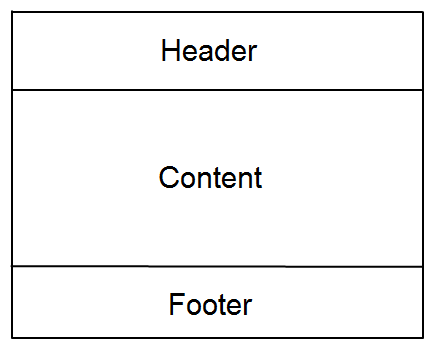
\includegraphics[width=0.3\textwidth]{Grafiken/Template.png}
			\caption{Standard-Template für alle Facelets}
		\end{figure}
		
		\paragraph{navigation.xhtml} \hypertarget{navigation}
		RS\\
		\begin{itemize}
			\item \textbf{Beschreibung:} Hier kann, abhängig von der Benutzerrolle, durch die Seite navigiert werden.
			\item \textbf{Links:}
			\begin{itemize}
				\item Suche: Navigiert zur Kurse durchsuchen Seite. \hyperlink{search}{search.xhtml}
				\item Sprache Deutsch: Ändert die angezeigte Sprache zu Deutsch.
				\item Sprache Englisch: Ändert die angezeigte Sprache zu Englisch.
				\item Profil (Benutzer): Navigiert zum eigenen Profil. \hyperlink{profile}{profile.xhtml}
				\item Meine Kurse (Benutzer): Navigiert zur Anzeige der eigenen Kurse. \hyperlink{myCourses}{myCourses.xhtml}
				\item Terminplaner (Benutzer): Navigiert zum persönlichen Terminplaner. \hyperlink{scheduler}{scheduler.xhtml}
				\item Seitenverwaltung (Administrator): Lässt den Seitenadministrator zur Seitenverwaltung navigieren. \hyperlink{adminManagement}{adminManagement.xhtml}
				\item Benutzer aktivieren: (Kursleiter, Administrator): Navigiert zur Benutzer aktivieren Seite. \hyperlink{activateUsers}{activateUsers.xhtml}
			\end{itemize}
			\begin{center}
				\begin{longtable}{|p{4cm} |p{6cm} |}

					\hline \multicolumn{1}{|c|}{\textbf{Link}} & \multicolumn{1}{|c|}{\textbf{\"{U}bergabeparameter}} \\ \hline
					\endfirsthead
					\hline
					\endlastfoot

					\textit{Suche} & ...\\ \hline
					\textit{Sprache Deutsch} & ...\\ \hline
					\textit{Sprache Englisch} & ...\\ \hline
					\textit{Profil (B)} & ...\\ \hline
					\textit{Meine Kurse (B)} & ...\\ \hline
					\textit{Terminplaner (B)} & ...\\ \hline
					\textit{Seitenverwaltung (A)} & ...\\ \hline
					\textit{Benutzer aktivieren (K, A)} & ...\\ \hline
				\end{longtable}
			\end{center}

			\item \textbf{Buttons:}
				\begin{itemize}
					\item Logout (Benutzer, wenn eingeloggt): Loggt den aktuellen eingeloggten Benutzer aus. \\ Zugehörige Methode: logout()
					\item Anmelden (Anonym): Navigiert zur Registrierungs- und Anmeldeseite. \hyperlink{authenticate}{authenticate.xhtml} \\ Zugehörige Methode: login()
				\end{itemize}
				\begin{center}
					\begin{longtable}{|p{4cm} |p{4cm} | p{4cm}|}
					
						\hline \multicolumn{1}{|c|}{\textbf{Button}} & \multicolumn{1}{|c|}{\textbf{Methode}} & \multicolumn{1}{|c|}{\textbf{\"{U}bergabeparameter}} \\ \hline
						\endfirsthead
						\hline
						\endlastfoot
					
							\textit{Logout (B)} & ... & ... \\ \hline
							\textit{Anmelden} & ... & ... \\ \hline
					\end{longtable}
				\end{center}
			\item \textbf{Inputs:} -
			\item \textbf{Outputs:}
				\begin{itemize}
					\item Logo: Zeigt verkleinertes, vom Administrator definiertes Logo der Website. Beim klick gelangt der Nutzer zur Startseite \hyperlink{index}{index.xhtml}.
				\end{itemize}
				\begin{center}
					\begin{longtable}{|p{5cm} | p{4cm}|p{3cm}|}
						
						\hline \multicolumn{1}{|c|}{\textbf{Ausgabefeld}} & \multicolumn{1}{|c|}{\textbf{Typ}}  &  \multicolumn{1}{|c|}{\textbf{ID}} \\ \hline
						\endfirsthead
						\hline
						\endlastfoot
						\textit{Logo}  & ... & ... \\ \hline
					\end{longtable}
				\end{center}
			\item \textbf{BackingBean:}
				\begin{itemize}
					\item Navigation.java
				\end{itemize}
		\end{itemize}
		
		\paragraph{footer.xhtml} \hypertarget{footer}
		RS\\
		\begin{itemize}
			\item \textbf{Beschreibung:} Dieses Facelet dient der Darstellung des Footers.
			\item \textbf{Links:} -
			\item \textbf{Buttons:}
			\begin{itemize}
				\item AGB: Navigiert zum Facelet mit den Allgemeinen Geschäftsbedingungen, also \hyperlink{agb}{agb.xhtml}. Zugehörige Methode: loadAGBPage()
				\item Impressum: Navigiert zum Facelet mit dem Impressum der Webanwendung, also \hyperlink{imprint}{imprint.xhtml}. Zugehörige Methode: loadImprintPage()
				\item Hilfe: Navigiert zur Hilfeseite, also COMPLETEuserHelp.html. Zugehörige Methode: loadHelpPage()
			\end{itemize}
			\begin{center}
				\begin{longtable}{|p{4cm} |p{4cm} | p{4cm}|}
					
					\hline \multicolumn{1}{|c|}{\textbf{Button}} & \multicolumn{1}{|c|}{\textbf{Methode}} & \multicolumn{1}{|c|}{\textbf{\"{U}bergabeparameter}} \\ \hline
					\endfirsthead
					\hline
					\endlastfoot

						\textit{AGB} & ... & ... \\ \hline
						\textit{Impressum} & ... & ... \\ \hline
						\textit{Hilfe} & ... & ... \\ \hline
				\end{longtable}
			\end{center}
			\item \textbf{Inputs:} -
			\item \textbf{Outputs:} -
			\item \textbf{BackingBean:}
			\begin{itemize}
				\item Footer.java
			\end{itemize}
		\end{itemize}
		
		\paragraph{template.xhtml} \hypertarget{template}
		RS\\
		\begin{itemize}
			\item \textbf{Beschreibung:} Dieses Facelet dient der einheitlichen Darstellung und Struktur aller Facelets im System. Letztere ist in Abbildung 4.1 genauer dargestellt.
			\item \textbf{Links:} -
			\item \textbf{Buttons:} -
			\item \textbf{Inputs:}
			\begin{itemize}
				\item Navigation: Bindet \hyperlink{navigation}{navigation.xhtml} in den Header ein.
				\item Footer: Bindet \hyperlink{footer}{footer.xhtml} in den Footer ein.
			\end{itemize}
			\begin{center}
				\begin{longtable}{|p{3cm} |p{5cm} | p{4cm}|p{3cm}|}
						
					\hline \multicolumn{1}{|c|}{\textbf{Eingabefeld}} & \multicolumn{1}{|c|}{\textbf{Backing-Bean-Attribute}} & \multicolumn{1}{|c|}{\textbf{Typ}}  &  \multicolumn{1}{|c|}{\textbf{ID}} \\ \hline
					\endfirsthead
					\hline
					\endlastfoot
					\textit{Navigation} & ... & ... & ... \\ \hline
					\textit{Footer} & ... & ... & ... \\ \hline
				\end{longtable}
			\end{center}
			\item \textbf{Outputs:} -
			\item \textbf{BackingBean:} -
		\end{itemize}
		
		\section{Facelets}
		
		\subsection{open}
		
		\subsubsection{common}
		
		\paragraph{errorPage.xhtml} \hypertarget{errorPage}
		KH\\
			\begin{itemize}
				\item \textbf{Beschreibung:} Der Benutzer wird auf diese Seite weitergeleitet, wenn Exceptions auftreten, auf die der Nutzer keinen Einfluss hat. Die entsprechende Fehlermeldung wird dann angezeigt.
				\item \textbf{Links:}
					\begin{itemize}
						\item Startseite: Über diesen Link gelangt der Benutzer zurück zur Startseite. (\hyperlink{index}{index.xhtml})
					\end{itemize}
					
					\begin{center}
						\begin{longtable}{|p{4cm} |p{6cm} |}
							
							\hline \multicolumn{1}{|c|}{\textbf{Link}} & \multicolumn{1}{|c|}{\textbf{\"{U}bergabeparameter}} \\ \hline
							\endfirsthead
							\hline
							\endlastfoot
							
							\textit{Startseite } & ...\\ \hline
						\end{longtable}
					\end{center}
					
				\item \textbf{Buttons:} -
				\item \textbf{Inputs:} -
				\item \textbf{Outputs:} -			
				\item \textbf{BackingBean:} -	
			\end{itemize}
		
		\paragraph{index.xhtml} \hypertarget{index}
		RS\\
		\begin{itemize}
			\item \textbf{Beschreibung:} Dieses Facelet stellt die Startseite des Systems dar.
			\item \textbf{Links:}
			\begin{itemize}
				\item Gesamtes Kursangebot, \hyperlink{search}{search.xhtml}
			\end{itemize}
			\item \textbf{Buttons:} -
			\item \textbf{Inputs:} -
			\item \textbf{Outputs:}
			\begin{itemize}
				\item Logo der Website
			\end{itemize}
			\item \textbf{BackingBean:} -
		\end{itemize}
		
		\paragraph{authenticate.xhtml} \hypertarget{authenticate}
		KH\\
		\begin{itemize}
			\item \textbf{Beschreibung:}
			Auf dieser Seite kann man sich im System anmelden, ein neues Benutzerkonto generieren oder ein neues Passwort anfordern.
			\item \textbf{Links:} -
			\item \textbf{Buttons:}
			\begin{itemize}
				\item Registrieren: Durch Drücken dieses Buttons wird der neue Benutzer mit den eingegebenen Daten im System gespeichert und es wird eine Bestätigungsmail mit dem Verifizierungslink an die angegebene E-Mail-Adresse verschickt, sofern alle Daten korrekt eingegeben wurden. \\ Zugehörige Methode: registerUser()
				\item Anmelden: Durch Drücken dieses Buttons wird der registrierte Benutzer im System angemeldet und auf die Seite 'Meine Kurse' (\hyperlink{myCourses}{myCourses.xhtml}) weitergeleitet, sofern Benutzername und Passwort korrekt eingegeben wurden. \\ Zugehörige Methode: login()
				\item Passwort vergessen: Durch Drücken dieses Buttons wird an die angegebene E-Mail-Adresse ein automatisch generiertes Passwort geschickt, sofern die Adresse im System existiert. \\ Zugehörige Methode: resetPassword()
			\end{itemize}
			
			\begin{center}
				\begin{longtable}{|p{4cm} |p{4cm} | p{4cm}|}
					
					\hline \multicolumn{1}{|c|}{\textbf{Button}} & \multicolumn{1}{|c|}{\textbf{Methode}} & \multicolumn{1}{|c|}{\textbf{\"{U}bergabeparameter}} \\ \hline
					\endfirsthead
					\hline
					\endlastfoot
					
						\textit{Registrieren } & registerUser() & ... \\ \hline
						\textit{Anmelden } & login() & ... \\ \hline
						\textit{Passwort vergessen } & resetPassword() & ... \\ \hline
				\end{longtable}
			\end{center}
			
			\item \textbf{Inputs:}
			\begin{itemize}
				\item Anrede (Registrierung): Hier wählt der Benutzer die Anrede 'Herr' oder 'Frau' aus.
				\item Vorname (Registrierung): Hier trägt der Benutzer seinen Vornamen ein.
				\item Name (Registrierung): Hier gibt der Benutzer seinen Namen ein.
				\item Benutzername (Registrierung): Hier gibt der Benutzer einen Benutzernamen ein.
				\item Passwort (Registrierung): Hier trägt der Benutzer ein Passwort ein.
				\item Passwort bestätigen (Registrierung): Hier gibt der Benutzer das gleiche Passwort erneut ein zur Bestätigung.
				\item Geburtstag (Registrierung): Hier gibt der Benutzer sein Geburtsdatum ein.
				\item Straße/Hausnummer (Registrierung): Hier gibt der Benutzer seine Straße und seine Hausnummer ein.
				\item Stadt (Registrierung): Hier trägt der Benutzer seine Stadt ein.
				\item Postleitzahl (Registrierung): Hier trägt der Benutzer seine Postleitzahl ein.
				\item Land (Registrierung): Hier trägt der Benutzer sein Heimatland ein.
				\item E-Mail-Adresse (Registrierung): Hier gibt der Benutzer seine E-Mail-Adresse ein.
				\item AGBs bestätigen (Registrierung): Durch Setzten des Häkchens bestätigt der Benutzer die AGBs. 
				\item Benutzername (Anmeldung): Der Benutzer gibt seinen Benutzernamen ein, mit dem er sich registriert hat.
				\item Passwort (Anmeldung): Der Benutzer gibt sein Passwort ein, mit dem er sich registriert hat.
				\item E-Mail-Adresse (Passwort vergessen): Der Benutzer gibt seine im System bereits gespeicherte E-Mailadresse ein.
				
				\begin{center}
					\begin{longtable}{|p{3cm} |p{5cm} | p{4cm}|p{3cm}|}
						
						\hline \multicolumn{1}{|c|}{\textbf{Eingabefeld}} & \multicolumn{1}{|c|}{\textbf{Backing-Bean-Attribute}} & \multicolumn{1}{|c|}{\textbf{Typ}}  &  \multicolumn{1}{|c|}{\textbf{ID}} \\ \hline
						\endfirsthead
						\hline
						\endlastfoot
							\textit{Anrede (R)} & - & selectOneMenu & anrede \\ \hline
							\textit{Vorname (R)} & - & inputText & vorname \\ \hline
							\textit{Name (R)} & - & inputText & name \\ \hline
							\textit{Benutzername (R)} & - & inputText & benutzername\\ \hline
							\textit{Passwort (R)} & - & inputSecret & passwort \\ \hline
							\textit{Passwort bestätigen (R)} &- & inputSecret & bestätigungs- passwort\\ \hline
							\textit{Geburtstag (R)} & - & inputText & geburtstag \\ \hline
							\textit{Straße/ Hausnummer (R)} & - & inputText & straße\\ \hline
							\textit{Stadt (R)} & - & inputText & stadt \\ \hline
							\textit{Postleitzahl (R)} & - & inputText & postleitzahl \\ \hline
							\textit{Land (R)} & - & inputText & land \\ \hline
							\textit{E-Mail-Adresse (R)} & - & inputText & mail\\ \hline
							\textit{AGBs bestätigen (R)} & - & selectBooleanCheckbox & agb \\ \hline
							\textit{Benutzername (A)} & - & inputText & anmeldungs- benutzername \\ \hline
							\textit{Passwort (A)} & - & inputSecret & anmeldungs- passwort \\ \hline
							\textit{E-Mail-Adresse (Passwort vergessen)} & - & inputText & Passwortmail \\ \hline
					\end{longtable}
				\end{center}
				
				\begin{center}
					\begin{longtable}{|p{3cm} |p{8cm} | p{5cm}|}
						
						\hline \multicolumn{1}{|c|}{\textbf{Eingabefeld}} & \multicolumn{1}{|c|}{\textbf{Validator}} & \multicolumn{1}{|c|}{\textbf{Konverter}} \\ \hline
						\endfirsthead
						\hline
						\endlastfoot
						\textit{Anrede (R)} & validateRequired & ...  \\ \hline
						\textit{Vorname (R)} & validateLength (minimum ="", maximum =""), validateRequired & ... \\ \hline
						\textit{Name (R)} & validateLength (minimum ="", maximum =""), validateRequired & ...  \\ \hline
						\textit{Benutzername (R)} & UserNameValidator, validateLength (minimum ="", maximum =""), validateRegex (pattern =""), validateRequired  & ... \\ \hline
						\textit{Passwort (R)} & PasswordValidator, validateRequired & ...  \\ \hline
						\textit{Passwort bestätigen (R)} & confirmPasswordValidator, validateRequired & ... \\ \hline
						\textit{Geburtstag (R)} & DateOfBirthValidator, validateRequired & convertDateTime  \\ \hline
						\textit{Straße/ Hausnummer (R)} & validateLength (minimum ="", maximum =""), validateRequired & ... \\ \hline
						\textit{Stadt (R)} & validateLength (minimum ="", maximum =""), validateRequired & ...  \\ \hline
						\textit{Postleitzahl (R)} & validateLength (minimum ="", maximum =""), validateRequired & ... \\ \hline
						\textit{Land (R)} & validateLength (minimum ="", maximum =""), validateRequired & ...  \\ \hline
						\textit{E-Mail-Adresse (R)} & EMailValidator, validateLength (minimum ="", maximum =""), validateRequired & ... \\ \hline
						\textit{AGBs bestätigen (R)} & - & ...  \\ \hline
						\textit{Benutzername (A)} & validateRequired & ...  \\ \hline
						\textit{Passwort (A)} & validateRequired & ...  \\ \hline
						\textit{E-Mail-Adresse (Passwort vergessen)} & validateRequired & ... \\ \hline
					\end{longtable}
				\end{center}
				
				
			\end{itemize}
			\item \textbf{Outputs:} 
			\begin{itemize}
				\item Anrede Fehlermeldung (Registrierung): Ausgabe der Fehlermeldungen zu den Validatoren des Eingabefeldes.
				\item Vorname Fehlermeldung (Registrierung): Ausgabe der Fehlermeldungen zu den Validatoren des Eingabefeldes.
				\item Name Fehlermeldung (Registrierung): Ausgabe der Fehlermeldungen zu den Validatoren des Eingabefeldes.
				\item Benutzername Fehlermeldung (Registrierung): Ausgabe der Fehlermeldungen zu den Validatoren des Eingabefeldes.
				\item Passwort Fehlermeldung (Registrierung): Ausgabe der Fehlermeldungen zu den Validatoren des Eingabefeldes.
				\item Passwort bestätigen Fehlermeldung (Registrierung): Ausgabe der Fehlermeldungen zu den Validatoren des Eingabefeldes.
				\item Geburtstag Fehlermeldung (Registrierung): Ausgabe der Fehlermeldungen zu den Validatoren des Eingabefeldes.
				\item Straße/Hausnummer Fehlermeldung (Registrierung): Ausgabe der Fehlermeldungen zu den Validatoren des Eingabefeldes.
				\item Stadt Fehlermeldung (Registrierung): Ausgabe der Fehlermeldungen zu den Validatoren des Eingabefeldes.
				\item Postleitzahl Fehlermeldung (Registrierung): Ausgabe der Fehlermeldungen zu den Validatoren des Eingabefeldes.
				\item Land Fehlermeldung (Registrierung): Ausgabe der Fehlermeldungen zu den Validatoren des Eingabefeldes.
				\item E-Mail-Adresse Fehlermeldung (Registrierung): Ausgabe der Fehlermeldungen zu den Validatoren des Eingabefeldes.
				\item AGBs bestätigen Fehlermeldung (Registrierung): Ausgabe der Fehlermeldungen zu den Validatoren des Eingabefeldes.
				\item Benutzername Fehlermeldung (Anmeldung): Ausgabe der Fehlermeldungen zu den Validatoren des Eingabefeldes.
				\item Passwort Fehlermeldung (Anmeldung): Ausgabe der Fehlermeldungen zu den Validatoren des Eingabefeldes.
				\item E-Mail-Adresse Fehlermeldung (Passwort vergessen): Ausgabe der Fehlermeldungen zu den Validatoren des Eingabefeldes.
			\end{itemize}
			
				\begin{center}
					\begin{longtable}{|p{5cm} | p{4cm}|p{5cm}|}
						
						\hline \multicolumn{1}{|c|}{\textbf{Ausgabefeld}} & \multicolumn{1}{|c|}{\textbf{Typ}}  &  \multicolumn{1}{|c|}{\textbf{ID}} \\ \hline
						\endfirsthead
						\hline
						\endlastfoot
						\textit{Anrede Fehlermeldung (R)}  & outputText & anredefehler \\ \hline
						\textit{Vorname Fehlermeldung (R)}  & outputText & vornamenfehler \\ \hline
						\textit{Name Fehlermeldung (R)} & outputText & namenfehler \\ \hline
						\textit{Benutzername Fehlermeldung (R)}& outputText & nutzernamenfehler\\ \hline
						\textit{Passwort Fehlermeldung (R)}& outputText & passwortfehler\\ \hline
						\textit{Passwort bestätigen Fehlermeldung (R)}& outputText & bestätigungspwfehler\\ \hline
						\textit{Geburtstag  Fehlermeldung(R)} & outputText & geburtstagsfehler \\ \hline
						\textit{Straße/ Hausnummer Fehlermeldung (R)}& outputText & straßenfehler\\ \hline
						\textit{Stadt Fehlermeldung (R)}& outputText & stadtfehler \\ \hline
						\textit{Postleitzahl Fehlermeldung (R)} & outputText & postleitzahlfehler \\ \hline
						\textit{Land Fehlermeldung (R)} & outputText & landfehler \\ \hline
						\textit{E-Mail-Adresse Fehlermeldung (R)} & outputText & mailfehler\\ \hline
						\textit{AGBs bestätigen Fehlermeldung (R)} & outputText & agbfehler \\ \hline
						\textit{Benutzername Fehlermeldung (A)}& outputText & anmeldenamefehler \\ \hline
						\textit{Passwort Fehlermeldung (A)} &  outputText & anmeldepwfehler \\ \hline
						\textit{E-Mail-Adresse Fehlermeldung (Passwort vergessen)}  & outputText & mailpw \\ \hline
					\end{longtable}
				\end{center}
			
			\item \textbf{BackingBean:}
				\begin{itemize}
					\item AuthenticateUser.java
					\item RegisterUser.java
					\item LostPassword.java
				\end{itemize}
		\end{itemize}
		
		\paragraph{imprint.xhtml} \hypertarget{imprint}
		KH\\
		\begin{itemize}
			\item \textbf{Beschreibung:} Auf dieser Seite kann das Impressum angezeigt werden.
			\item \textbf{Links:} -
			\item \textbf{Buttons:} -
			\item \textbf{Inputs:} -
			\item \textbf{Outputs:} 
				\begin{itemize}
					\item	Anzeige des Impressums, welches vom Administrator festgelegt wurde.
				\end{itemize}
				
				\begin{center}
					\begin{longtable}{|p{5cm} | p{4cm}|p{3cm}|}
						
						\hline \multicolumn{1}{|c|}{\textbf{Ausgabefeld}} & \multicolumn{1}{|c|}{\textbf{Typ}}  &  \multicolumn{1}{|c|}{\textbf{ID}} \\ \hline
						\endfirsthead
						\hline
						\endlastfoot
						\textit{Impressum}  & outputText & impressumzeigen \\ \hline
					\end{longtable}
				\end{center}
				
			\item \textbf{BackingBean:} -
		\end{itemize}
		
		\paragraph{agb.xhtml} \hypertarget{agb}
		RS\\
		\begin{itemize}
			\item \textbf{Beschreibung:} Dieses Facelet dient der Anzeige der Allgemeinen Geschäftsbedingungen.
			\item \textbf{Links:} -
			\item \textbf{Buttons:} -
			\item \textbf{Inputs:} -
			\item \textbf{Outputs:}
			\begin{itemize}
				\item von Betreibern festgelegte Allgemeine Geschäftsbedingungen.
			\end{itemize}
			\item \textbf{BackingBean:} -
		\end{itemize}
		
		
		\subsubsection{courses}
		
		\paragraph{search.xhtml} \hypertarget{search}
		RS\\
		\begin{itemize}
			\item \textbf{Beschreibung:} Hier können alle Kurse angezeigt und durchsucht werden.
			\item \textbf{Links:} -
			\item \textbf{Buttons:}
			\begin{itemize}
				\item Anzeigen: Zeigt die Angebote im ausgewählten Zeitraum an. \\ Zugehörige Methode: displayCoursesInSpecificPeriod()
				\item Suchen: Durchsucht die Website nach dem eingegebenen Suchbegriff mittels gewählten Suchobjekt. \\ Zugehörige Methode: search()
			\end{itemize}
			\item \textbf{Inputs:}
			\begin{itemize}
				\item Angebotszeitraum: Ermöglicht eine genauere Anzeige des Kursangebots, entweder Tagesangebot, Wochenangebot oder das gesamte Angebot. Die detaillierteren Suchoptionen sind nur für registrierte Benutzer verfügbar.
				\item Suchobjekt (abhängig von Benutzerrolle): Ermöglicht eine genauere Suche, beispielsweise nach Kursen, Kursleitern oder Kurs-ID.
			\end{itemize}
			\item \textbf{Outputs:}
			\begin{itemize}
				\item Tabelle mit Ergebnissen der Suche.
				\item Schaltfläche um zwischen Ergebnissen zu Blättern.
			\end{itemize}
			\item \textbf{BackingBean:}
			\begin{itemize}
				\item SearchCourse.java
			\end{itemize}
		\end{itemize}
		
		\paragraph{courseDetails.xhtml} \hypertarget{courseDetails}
		RS\\
		\begin{itemize}
			\item \textbf{Beschreibung:} Zur genaueren Betrachtung eines einzelnen Kurses wird dieses Facelet benötigt.
			\item \textbf{Links:} -
			\item \textbf{Buttons:}
			\begin{itemize}
				\item Anmelden (Benutzer, noch nicht angemeldet): Meldet den Benutzer zum Kurs an. \\ Zugehörige Methode: signUpForCourse()
				\item Abmelden (Benutzer, wenn angemeldet): Meldet den Benutzer vom Kurs ab. \\ Zugehörige Methode: signOffFromCourse()
				\item Teilnehmer anzeigen (Benutzer): Zeigt die zum Kurs angemeldeten Benutzer an. \hyperlink{listParticipants}{listParticipants.xhtml} \\ Zugehörige Methode: loadParticipantsPage()
				\item Alle auswählen (Benutzer, zum Kurs angemeldet): Wählt alle Kurseinheiten des Kurses aus. \\ Zugehörige Methode: selectAllCourseUnits()
				\item Speichern (Benutzer, zum Kurs angemeldet): Speichert alle ausgewählten Kurseinheiten und meldet den Nutzer dazu an. \\ Zugehörige Methode: signUpForCourseUnits()
				\item Bearbeiten (Administrator, noch nicht im Bearbeitungsmodus): Ermöglicht die Bearbeitung der einzelnen Kursdetails. \\ Zugehörige Methode: editCourse()
				\item Speichern (Administrator, im Bearbeitungsmodus): Speichert alle vorgenommenen Kursänderungen. \\ Zugehörige Methode: saveCourse()
				\item Hinzufügen (Administrator): Fügt einen Kursleiter zum Kurs hinzu. Zugehörige Methode: addCourseLeader()
				\item Kurseinheit anlegen (Kursleiter): Erstellt eine neue Kurseinheit zum Kurs. \hyperlink{editCourseUnit}{editCourseUnit.xhtml} \\ Zugehörige Methode: loadCreateCourseUnitPage()
				\item Kurseinheit bearbeiten (Kursleiter): Ermöglicht die Bearbeitung einer einzelnen Kurseinheit. \hyperlink{editCourseUnit}{editCourseUnit.xhtml} \\ Zugehörige Methode: loadEditCourseUnitPage()
				\item Kurs löschen (Administrator): Löscht den Kurs. \\ Zugehörige Methode: deleteCourse()
			\end{itemize}
			\begin{center}
				\begin{longtable}{|p{4cm} |p{6cm} | p{4cm}|}
						
					\hline \multicolumn{1}{|c|}{\textbf{Button}} & \multicolumn{1}{|c|}{\textbf{Methode}} & \multicolumn{1}{|c|}{\textbf{\"{U}bergabeparameter}} \\ \hline
					\endfirsthead
					\hline
					\endlastfoot
			
					\textit{Anmelden (B)} & ... & ... \\ \hline
					\textit{Abmelden (B)} &  ... & ... \\ \hline
					\textit{Benutzer anzeigen (B)} & ... & ... \\ \hline
					\textit{Alle auswählen (B)} & ... & ... \\ \hline
					\textit{Speichern (B)} & ... & ... \\ \hline
					\textit{Bearbeiten (A)} & ... & ... \\ \hline
					\textit{Speichern (A)} & ... & ... \\ \hline
					\textit{Hinzufügen (A)} & ... & ... \\ \hline
					\textit{Kurseinheit anlegen (K)} & ... & ... \\ \hline
					\textit{Kurseinheit bearbeiten (K)} & ... & ... \\ \hline
					\textit{Kurs löschen (A)} & ... & ... \\ \hline
				\end{longtable}
			\end{center}
			\item \textbf{Inputs:}
			\begin{itemize}
				\item Kursnews erhalten: Trägt Benutzer bei Anmeldung zum Kurs in die Kursnews ein.
				\item Kurseinheit auswählen: Wählt Kurseinheit aus, zu der sich der Nutzer anmelden möchte.
				\item Kursleiter auswählen (Administrator): Wählt Kursleiter aus, welcher gelöscht werden soll.
				\item Kursleiter Name (Administrator): Eingabefeld für den Namen eines neuen Kursleiters.
				\item Kursleiter E-Mail (Administrator): Eingabefeld für die E-Mail Adresse eines neuen Kursleiters.
				\item Kursbeschreibung (Administrator): Eingabefeld für die Kursbeschreibung.
				\item Minimale Teilnehmerzahl (Administrator): Eingabefeld für die minimale Teilnehmerzahl des Kurses.
				\item Maximale Teilnehmerzahl (Administrator): Eingabefeld für die maximale Teilnehmerzahl des Kurses.
				\item Startdatum (Administrator): Eingabefeld für das Startdatum des Kurses.
				\item Enddatum (Administrator): Eingabefeld für das Enddatum des Kurses.
			\end{itemize}
				\begin{center}
					\begin{longtable}{|p{3cm} |p{4cm} | p{4cm}|p{3cm} |p{2cm}|}
						
						\hline \multicolumn{1}{|c|}{\textbf{Feld}} & \multicolumn{1}{|c|}{\textbf{Action}} & \multicolumn{1}{|c|}{\textbf{Validatoren}}  &  \multicolumn{1}{|c|}{\textbf{Konverter}} &  \multicolumn{1}{|c|}{\textbf{ID}} \\ \hline
						\endfirsthead
						\hline
						\endlastfoot
						\textit{Kursnews erhalten} & ... & ... & ... & ..\\ \hline
						\textit{Kurseinheit auswählen} & ... & ... & ... & ..\\ \hline
						\textit{Kursleiter auswählen (A)} & ... & ... & ... & ..\\ \hline
						\textit{Kursleiter Name (A)} & ... & ... & ... & ..\\ \hline
						\textit{Kursleiter E-Mail (A)} & ... & ... & ... & ..\\ \hline
						\textit{Kursbeschreibung (A)} & ... & ... & ... & ..\\ \hline
						\textit{Minimale Teilnehmerzahl (A)} & ... & ... & ... & ..\\ \hline
						\textit{Maximale Teilnehmerzahl (A)} & ... & ... & ... & ..\\ \hline
						\textit{Startdatum (A)} & ... & ... & ... & ..\\ \hline
						\textit{Enddatum (A)} & ... & ... & ... & ..\\ \hline
					\end{longtable}
				\end{center}
			\item \textbf{Outputs:}
			\begin{itemize}
				\item Tabelle Kursleiter: Tabelle mit den Kontaktinformationen der/des Kursleiters.
				\item Tabelle Kurseinheiten: Tabelle mit allen Kurseinheiten des Kurses und zugehörigen Informationen wie Ort, Preis oder Datum.
				\item Kurs-ID: Zeigt die zum Kurs zugehörige ID an.
				\item Kursbeschreibung: Zeigt die Beschreibung zum Kurs an.
				\item Minimale Teilnehmerzahl: Zeigt die für den Kurs minimale Teilnehmerzahl an.
				\item Maximale Teilnehmerzahl: Zeigt die für den Kurs maximale Teilnehmerzahl an.
				\item Fehlermeldung zu den einzelnen Eingabefeldern, bei falscher Eingabe.
			\end{itemize}
					\begin{center}
						\begin{longtable}{|p{5cm} | p{4cm}|p{3cm}|}
							
							\hline \multicolumn{1}{|c|}{\textbf{Ausgabefeld}} & \multicolumn{1}{|c|}{\textbf{Typ}}  &  \multicolumn{1}{|c|}{\textbf{ID}} \\ \hline
							\endfirsthead
							\hline
							\endlastfoot
							\textit{Tabelle Kursleiter}  & dataTable & ... \\ \hline
							\textit{Tabelle Kurseinheiten}  & dataTable & ... \\ \hline
							\textit{Kurs-ID}  & outputText & ... \\ \hline
							\textit{Kursbeschreibung}  & outputText & ... \\ \hline
							\textit{Minimale Teilnehmerzahl}  & outputText & ... \\ \hline
							\textit{Maximale Teilnehmerzahl}  & outputText & ... \\ \hline
							\textit{Kursleiter Name Fehlermeldung}  & outputText & ... \\ \hline
							\textit{Kursleiter E-Mail Fehlermeldung}  & outputText & ... \\ \hline
							\textit{Kursbeschreibung Fehlermeldung}  & outputText & ... \\ \hline
							\textit{Minimale Teilnehmerzahl Fehlermeldung}  & outputText & ... \\ \hline
							\textit{Maximale Teilnehmerzahl Fehlermeldung}  & outputText & ... \\ \hline
							\textit{Startdatum Fehlermeldung}  & outputText & ... \\ \hline
							\textit{Enddatum Fehlermeldung}  & outputText & ... \\ \hline
						\end{longtable}
					\end{center}
			\item \textbf{BackingBean:}
			\begin{itemize}
				\item CourseDetail.java
				\item CourseManagement.java
			\end{itemize}
		\end{itemize}
		
		\subsection{users}
		
		\subsubsection{registeredUser}
		
		\paragraph{myCourses.xhtml} \hypertarget{myCourses}
		KH\\
		\begin{itemize}
			\item \textbf{Beschreibung:} Auf dieser Seite werden alle Kurse angezeigt, in die der Teilnehmer eingetragen ist.
			\item \textbf{Links:}
				\begin{itemize}
					\item Kurstitel: Über die Kurstitel gelangt der Benutzer auf die jeweilige Kursdetailseite. (\hyperlink{courseDetails}{courseDetails.xhtml})
				\end{itemize}
				
				\begin{center}
					\begin{longtable}{|p{4cm} |p{6cm} |}
						
						\hline \multicolumn{1}{|c|}{\textbf{Link}} & \multicolumn{1}{|c|}{\textbf{\"{U}bergabeparameter}} \\ \hline
						\endfirsthead
						\hline
						\endlastfoot
						
						\textit{Kurstitel } & ...\\ \hline
					\end{longtable}
				\end{center}
				
			\item \textbf{Buttons:} -
			\item \textbf{Inputs:} -
			\item \textbf{Outputs:}
				\begin{itemize}
					\item Tabelle Auflistung aller Kurse: Hier werden dem Benutzer alle seine angemeldeten Kurse angezeigt.
				\end{itemize}
				
				\begin{center}
					\begin{longtable}{|p{5cm} | p{4cm}|p{3cm}|}
						
						\hline \multicolumn{1}{|c|}{\textbf{Ausgabefeld}} & \multicolumn{1}{|c|}{\textbf{Typ}}  &  \multicolumn{1}{|c|}{\textbf{ID}} \\ \hline
						\endfirsthead
						\hline
						\endlastfoot
						\textit{Kurstabelle}  & dataTable & kurstabelle \\ \hline
					\end{longtable}
				\end{center}
				
			\item \textbf{BackingBean:}
				\begin{itemize}
					\item MyCourses.java
				\end{itemize}
		\end{itemize}
		
		\paragraph{profile.xhtml} \hypertarget{profile}
		KH\\
		\begin{itemize}
			\item \textbf{Beschreibung:} Auf dieser Seite werden die persönlichen Daten und der Kontostand des Benutzers angezeigt. Der Benutzer kann die Daten ändern und sein Konto aufladen. Der Kursleiter kann hier den Benutzer aktivieren, und der Administrator den Benutzer löschen.
			\item \textbf{Links:} -
			\item \textbf{Buttons:}
				\begin{itemize}
					\item Bearbeiten: Nach Klicken auf diesen Button können die persönlichen Daten geändert werden. Der Button trägt nun die Aufschrift 'Speichern' und ist mit dessen dazugehöriger Methode hinterlegt. \\ Zugehörige Methode: editUserData()
					\item Speichern: Durch Drücken dieses Buttons werden die vorgenommenen Änderungen gespeichert, sofern alle Daten korrekt eingegeben wurden. Bei Änderung der E-Mail-Adresse wird außerdem eine Bestätigungsmail mit einem Verifizierungslink verschickt. Bei erfolgreicher Speicherung erscheint der Button 'Bearbeiten' anstelle des Button 'Speichern'. \\ Zugehörige Methode: saveUserData()
					\item Durchsuchen: Durch Drücken dieses Buttons kann das eigene Dateiverzeichnis nach einem Bild durchsucht werden.
					\item Hochladen: Durch Drücken dieses Buttons wird das ausgewählte Profilbild hochgeladen. \\ Zugehörige Methode: uploadProfilPic()
					\item Konto aufladen: Durch Klicken dieses Buttons wird der Benutzer auf die Seite 'Kontoaufladung' (\hyperlink{buyCredits}{buyCredits.xhtml})  weitergeleitet. \\ Zugehörige Methode: depositMoneyPerCreditCard()
					\item Benutzer löschen: Durch Drücken dieses Buttons entfernt der Administrator diesen Benutzer aus dem System, oder der Benutzer kann sich selbst auf inaktiv setzen. \\ Zugehörige Methoden: deleteUser(), setUserInactive() 
				\end{itemize}
				
					\begin{center}
						\begin{longtable}{|p{4cm} |p{6cm} | p{4cm}|}
							
							\hline \multicolumn{1}{|c|}{\textbf{Button}} & \multicolumn{1}{|c|}{\textbf{Methode}} & \multicolumn{1}{|c|}{\textbf{\"{U}bergabeparameter}} \\ \hline
							\endfirsthead
							\hline
							\endlastfoot
							
							\textit{Bearbeiten } & editUserData() & ... \\ \hline
							\textit{Speichern } & saveUserData() & ... \\ \hline
							\textit{Duchsuchen } & - & ... \\ \hline
							\textit{Hochladen } & uploadProfilPic() & ... \\ \hline
							\textit{Kontoaufladen } & depositMoneyPerCreditCard() & ... \\ \hline
							\textit{Benutzer löschen} &  deleteUser(), setUserInactive()  & ... \\ \hline
						\end{longtable}
					\end{center}
				
			\item \textbf{Inputs:}
				\begin{itemize}
					\item Anrede: Hier kann der Benutzer seine Anrede ändern.
					\item Vorname: Hier kann der Benutzer seinen Vornamen ändern.
					\item Name: Hier kann der Benutzer seinen Namen ändern.
					\item Geburtstag: Hier kann der Benutzer sein Geburtsdatum ändern.
					\item Straße/Hausnummer: Hier kann der Benutzer seine Straße und Hausnummer ändern.
					\item Stadt: Hier kann der Benutzer seine Stadt ändern.
					\item Postleitzahl: Hier kann der Benutzer seine Postleitzahl ändern.
					\item Land: Hier kann der Benutzer seine Land ändern.
					\item E-Mail-Adresse: Hier kann der Benutzer seine E-Mail-Adresse ändern.
					\item Benutzername: Hier kann der Benutzer seinen Benutzernamen ändern.
					\item Passwort: Hier kann der Benutzer sein Passwort ändern.
					\item Passwort bestätigen: Hier muss der Benutzer sein geändertes Passwort bestätigen.
					\item Benutzerrolle: Hier kann der Administrator die Benutzerrolle eines Nutzers ändern.
					\item Profilbild Pfad: Hier kann der Benutzer sein Profilbild ändern.
				\end{itemize}
				
				\begin{center}
					\begin{longtable}{|p{3cm} |p{5cm} | p{4cm}|p{3cm}|}
						
						\hline \multicolumn{1}{|c|}{\textbf{Eingabefeld}} & \multicolumn{1}{|c|}{\textbf{Backing-Bean-Attribute}} & \multicolumn{1}{|c|}{\textbf{Typ}}  &  \multicolumn{1}{|c|}{\textbf{ID}} \\ \hline
						\endfirsthead
						\hline
						\endlastfoot
						\textit{Anrede} & UserProfil.User.salutation & selectOneMenu & anrede \\ \hline
						\textit{Vorname} & UserProfil.User.fistname & inputText & vorname \\ \hline
						\textit{Name} & UserProfil.User.lastname & inputText & name \\ \hline
						\textit{Geburtstag } & UserProfil.User.dateOfBirth & inputText & geburtstag \\ \hline
						\textit{Straße/ Hausnummer} & UserProfil.Address.street, UserProfil.Address.houseNumber  & inputText & straße\\ \hline
						\textit{Stadt} & UserProfil.Address.city & inputText & stadt \\ \hline
						\textit{Postleitzahl} & UserProfil.Address.zipCode & inputText & postleitzahl \\ \hline
						\textit{Land} & UserProfil.Address.country & inputText & land \\ \hline
						\textit{E-Mail-Adresse} & UserProfil.User.email & inputText & mail\\ \hline
						\textit{Benutzername} & UserProfil.User.username & inputText & benutzername \\ \hline
						\textit{Passwort} & UserProfil.User.password  & inputSecret & passwort \\ \hline
						\textit{Passwort bestätigen} & UserProfil.User.password & inputSecret & bestätigungs- passwort \\ \hline
						\textit{Benutzerrolle} & UserProfil.User.userRole & inputText & rolle \\ \hline
						\textit{Profilbild Pfad} & UserProfil.User.profilImage & inputText & bildpfad \\ \hline
					\end{longtable}
				\end{center}
				
				\begin{center}
					\begin{longtable}{|p{3cm} |p{8cm} | p{5cm}|}
						
						\hline \multicolumn{1}{|c|}{\textbf{Eingabefeld}} & \multicolumn{1}{|c|}{\textbf{Validator}} & \multicolumn{1}{|c|}{\textbf{Konverter}} \\ \hline
						\endfirsthead
						\hline
						\endlastfoot
						\textit{Anrede} & validateRequired & ... \\ \hline
						\textit{Vorname} & validateLength (minimum ="", maximum =""), validateRequired & ... \\ \hline
						\textit{Name} & validateLength (minimum ="", maximum =""), validateRequired & ...  \\ \hline
						\textit{Geburtstag} & DateOfBirthValidator, validateRequired & convertDateTime  \\ \hline
						\textit{Straße/ Hausnummer} & validateLength (minimum ="", maximum =""), validateRequired & ... \\ \hline
						\textit{Stadt} & validateLength (minimum ="", maximum =""), validateRequired & ...  \\ \hline
						\textit{Postleitzahl} & validateLength (minimum ="", maximum =""), validateRequired & ... \\ \hline
						\textit{Land} & validateLength (minimum ="", maximum =""), validateRequired & ...  \\ \hline
						\textit{E-Mail-Adresse} & EMailValidator, validateLength (minimum ="", maximum =""), validateRequired & ... \\ \hline
						\textit{Benutzername} & UserNameValidator, validateLength (minimum ="", maximum =""), validateRegex (pattern =""), validateRequired  & ... \\ \hline
						\textit{Passwort} & PasswordValidator, validateRequired & ...  \\ \hline
						\textit{Passwort bestätigen} & ConfirmPasswordValidator, validateRequired & ... \\ \hline
						\textit{Benutzerrolle} & validateRequired & ... \\ \hline
						\textit{Profilbild Pfad} & UserImageValidator & ... \\ \hline
					\end{longtable}
				\end{center}
				
				
			\item \textbf{Outputs:}
				\begin{itemize}
					\item Benutzer-ID: Ausgabe der automatisch generierten ID.
					\item Vorname Fehlermeldung: Ausgabe der Fehlermeldungen zu den Validatoren des Eingabefeldes.
					\item Name Fehlermeldung: Ausgabe der Fehlermeldungen zu den Validatoren des Eingabefeldes.
					\item Geburtstag Fehlermeldung: Ausgabe der Fehlermeldungen zu den Validatoren des Eingabefeldes.
					\item Straße/Hausnummer Fehlermeldung: Ausgabe der Fehlermeldungen zu den Validatoren des Eingabefeldes.
					\item Stadt Fehlermeldung: Ausgabe der Fehlermeldungen zu den Validatoren des Eingabefeldes.
					\item Postleitzahl Fehlermeldung: Ausgabe der Fehlermeldungen zu den Validatoren des Eingabefeldes.
					\item Land Fehlermeldung: Ausgabe der Fehlermeldungen zu den Validatoren des Eingabefeldes.
					\item E-Mail-Adresse Fehlermeldung: Ausgabe der Fehlermeldungen zu den Validatoren des Eingabefeldes.
					\item Benutzername Fehlermeldung: Ausgabe der Fehlermeldungen zu den Validatoren des Eingabefeldes.
					\item Passwort Fehlermeldung: Ausgabe der Fehlermeldungen zu den Validatoren des Eingabefeldes.
					\item Passwort bestätigen Fehlermeldung: Ausgabe der Fehlermeldungen zu den Validatoren des Eingabefeldes.
					\item Profilbild Fehlermeldung: Ausgabe der Fehlermeldungen zu den Validatoren des Eingabefeldes.
					\item Kontostand: Ausgabe des aktuellen Kontostandes.
					\item Tabelle Auflistung der Trainingskurse: Hier werden dem Kursleiter alle Kurse aufgelistet, die er leitet.
					\item Profilbild: Hier wird das Profilbild angezeigt.
				\end{itemize}
				
				\begin{center}
					\begin{longtable}{|p{5cm} | p{4cm}|p{5cm}|}
						
						\hline \multicolumn{1}{|c|}{\textbf{Ausgabefeld}} & \multicolumn{1}{|c|}{\textbf{Typ}}  &  \multicolumn{1}{|c|}{\textbf{ID}} \\ \hline
						\endfirsthead
						\hline
						\endlastfoot
						\textit{Benutzer-ID}  & outputText & nutzerid \\ \hline
						\textit{Vorname Fehlermeldung }  & outputText & vornamefehler \\ \hline
						\textit{Name Fehlermeldung } & outputText & namefehler \\ \hline
						\textit{Geburtstag  Fehlermeldung} & outputText & geburtstagsfehler \\ \hline
						\textit{Straße/ Hausnummer Fehlermeldung }& outputText & straßefehler\\ \hline
						\textit{Stadt Fehlermeldung }& outputText & stadtfehler \\ \hline
						\textit{Postleitzahl Fehlermeldung } & outputText & postleitzahlfehler \\ \hline
						\textit{Land Fehlermeldung } & outputText & landfehler \\ \hline
						\textit{E-Mail-Adresse Fehlermeldung} & outputText & mailfehler\\ \hline
						\textit{Benutzername Fehlermeldung }& outputText & nutzernamefehler \\ \hline
						\textit{Passwort Fehlermeldung} &  outputText & passwortfehler \\ \hline
						\textit{Passwort bestätigen Fehlermeldung}  & outputText & bestätigungspwfehler \\ \hline
						\textit{Profilbild Fehlermeldung} &  outputText & bildfehler \\ \hline
						\textit{Kontostand} &  outputText & kontostand \\ \hline
						\textit{Tabelle Trainingskurse} &  dataTable & trainingskurse \\ \hline
						\textit{Profilbild} &  graphicImage & bild \\ \hline
					\end{longtable}
				\end{center}
				
			\item \textbf{BackingBean:}
				\begin{itemize}
					\item UserProfile.java
					\item UserManagement.java				
				\end{itemize}
		\end{itemize}
		
		\paragraph{buyCredits.xhtml} \hypertarget{buyCredits}
		RS\\
		\begin{itemize}
			\item \textbf{Beschreibung:} Hier kann der Nutzer mittels Kreditkarte seinen systeminternen Kontostand erhöhen.
			\item \textbf{Links:} -
			\item \textbf{Buttons:}
			\begin{itemize}
				\item Konto aufladen: Führt die Kontoaufladung aus. \\ Zugehörige Methode: depositAmount()
			\end{itemize}
			\begin{center}
				\begin{longtable}{|p{4cm} |p{6cm} | p{4cm}|}
						
					\hline \multicolumn{1}{|c|}{\textbf{Button}} & \multicolumn{1}{|c|}{\textbf{Methode}} & \multicolumn{1}{|c|}{\textbf{\"{U}bergabeparameter}} \\ \hline
					\endfirsthead
					\hline
					\endlastfoot
			
					\textit{Konto aufladen} & depositAmount() & ... \\ \hline
				\end{longtable}
			\end{center}
			\item \textbf{Inputs:}
			\begin{itemize}
				\item CVC-Nummer: Prüfnummer der Kreditkarte.
				\item Ablaufdatum: Ablaufdatum der Kreditkarte.
				\item Nachname: Nachname des Nutzers zur Kontoaufladung.
				\item Vorname: Vorname des Nutzers zur Kontoaufladung.
				\item Kreditinstitut: Name des Kreditinstitutes des Nutzers zur Kontoaufladung.
				\item Kreditkartennummer: Nummer der Kreditkarte des Nutzers zur Kontoaufladung.
				\item Betrag: Geldbetrag, welcher auf das systeminterne Konto des Nutzers gebucht werden soll.
			\end{itemize}
				\begin{center}
					\begin{longtable}{|p{3cm} |p{4cm} | p{4cm}|p{3cm} |p{2cm}|}
						
						\hline \multicolumn{1}{|c|}{\textbf{Feld}} & \multicolumn{1}{|c|}{\textbf{Action}} & \multicolumn{1}{|c|}{\textbf{Validatoren}}  &  \multicolumn{1}{|c|}{\textbf{Konverter}} &  \multicolumn{1}{|c|}{\textbf{ID}} \\ \hline
						\endfirsthead
						\hline
						\endlastfoot
						\textit{CVC-Nummer} & ... & ... & ... & ..\\ \hline
						\textit{Ablaufdatum} & ... & ... & ... & ..\\ \hline
						\textit{Nachname} & ... & ... & ... & ..\\ \hline
						\textit{Vorname} & ... & ... & ... & ..\\ \hline
						\textit{Kredit-institut} & ... & ... & ... & ..\\ \hline
						\textit{Kreditkarten-nummer} & ... & ... & ... & ..\\ \hline
						\textit{Betrag} & ... & ... & ... & ..\\ \hline
					\end{longtable}
				\end{center}
			\item \textbf{Outputs:}
			\begin{itemize}
				\item Fehlermeldung zu den einzelnen Eingabefeldern, bei falscher Eingabe.
				\item Bestätigungsmeldung bei erfolgreicher Aufladung des Kontos.
			\end{itemize}
					\begin{center}
						\begin{longtable}{|p{5cm} | p{4cm}|p{3cm}|}
							
							\hline \multicolumn{1}{|c|}{\textbf{Ausgabefeld}} & \multicolumn{1}{|c|}{\textbf{Typ}}  &  \multicolumn{1}{|c|}{\textbf{ID}} \\ \hline
							\endfirsthead
							\hline
							\endlastfoot
							\textit{CVC-Nummer Fehlermeldung}  & outputText & ... \\ \hline
							\textit{Ablaufadtum Fehlermeldung}  & outputText & ... \\ \hline
							\textit{Nachname Fehlermeldung}  & outputText & ... \\ \hline
							\textit{Vorname Fehlermeldung}  & outputText & ... \\ \hline
							\textit{Kredit-Institut Fehlermeldung}  & outputText & ... \\ \hline
							\textit{Kreditkarten-nummer Fehlermeldung}  & outputText & ... \\ \hline
							\textit{Betrag Fehlermeldung}  & outputText & ... \\ \hline
						\end{longtable}
					\end{center}
			\item \textbf{BackingBean:}
			\begin{itemize}
				\item PayementOnline.java
			\end{itemize}
		\end{itemize}
		
		\paragraph{scheduler.xhtml} \hypertarget{scheduler}
		RS\\
		\begin{itemize}
			\item \textbf{Beschreibung:} Persönlicher Terminplaner mit anstehenden Kursen.
			\item \textbf{Links:}
			\begin{itemize}
				\item Wochenansicht vorwärts: Zeigt die Termine der nächsten Woche an.
				\item Wochenansicht rückwärts: Zeigt die Termine der letzten Woche an.
			\end{itemize}
			\item \textbf{Buttons:} -
			\item \textbf{Inputs:} -
			\item \textbf{Outputs:}
			\begin{itemize}
				\item Wochentabelle: Zeigt von Montag bis Sonntag alle belegten Kurseinheiten an. Orientiert sich am klassischen Stundenplan, also mit stündlicher Ansicht.
			\end{itemize}
			\item \textbf{BackingBean:}
			\begin{itemize}
				\item Scheduler.java
			\end{itemize}
		\end{itemize}
		
		\paragraph{leaderProfile.xhtml} \hypertarget{leaderProfile}
		KH\\
		\begin{itemize}
			\item \textbf{Beschreibung:} Auf dieser Seite werden die Daten des Kursleiters, mit Ausnahme von sensiblen Daten wie Passwort oder Kontostand, und die von ihm geleiteten Kurse angezeigt.
			\item \textbf{Links:} -
			\item \textbf{Buttons:} -
			\item \textbf{Inputs:} -
			\item \textbf{Outputs:} 
			\begin{itemize}
				\item Tabelle Auflistung Kursleiterdaten: Hier werden die Daten des Kursleiters und die von ihm geleiteten Kurse angezeigt.
			\end{itemize}
			
			\begin{center}
				\begin{longtable}{|p{5cm} | p{4cm}|p{3cm}|}
					
					\hline \multicolumn{1}{|c|}{\textbf{Ausgabefeld}} & \multicolumn{1}{|c|}{\textbf{Typ}}  &  \multicolumn{1}{|c|}{\textbf{ID}} \\ \hline
					\endfirsthead
					\hline
					\endlastfoot
					\textit{Tabelle Kursleiterdaten}  & dataTable & kursleiterdaten \\ \hline
				\end{longtable}
			\end{center}
			
			\item \textbf{BackingBean:}
			\begin{itemize}
				\item UserProfile.java			
			\end{itemize}
		\end{itemize}
		
		\paragraph{listParticipants.xhtml} \hypertarget{listParticipants}
		KH\\
		\begin{itemize}
			\item \textbf{Beschreibung:} Hier kann der registrierte Benutzer die Teilnehmer eines Kurses mit Benutzername und Profilbild ansehen. Dem Kursleiter werden zusätzlich die E-Mail-Adresse und die Information über den Erhalt von Kursnews angezeigt. Außerdem kann er einen Teilnehmer aus dem Kurs entfernen.
			\item \textbf{Links:} -
			\item \textbf{Buttons:}
			\begin{itemize}
				\item Löschen: Durch Drücken dieses Buttons kann der Kursleiter den entsprechenden Benutzer aus dem Kurs entfernen. \\ Zugehörige Methode: deleteUserFromCourse()
				
				\begin{center}
					\begin{longtable}{|p{4cm} |p{6cm} | p{4cm}|}
						
						\hline \multicolumn{1}{|c|}{\textbf{Button}} & \multicolumn{1}{|c|}{\textbf{Methode}} & \multicolumn{1}{|c|}{\textbf{\"{U}bergabeparameter}} \\ \hline
						\endfirsthead
						\hline
						\endlastfoot
						
						\textit{Löschen } & deleteUserFromCourse() & ... \\ \hline
					\end{longtable}
				\end{center}
				
			\end{itemize}
			\item \textbf{Inputs:}
			\begin{itemize}
				\item Entfernen: Durch Setzen des Häkchens wählt der Kursleiter diesen Benutzer aus, um ihn anschließend über den Button 'Löschen' zu entfernen.
				
				\begin{center}
					\begin{longtable}{|p{3cm} |p{5cm} | p{4cm}|p{3cm}|}
						
						\hline \multicolumn{1}{|c|}{\textbf{Eingabefeld}} & \multicolumn{1}{|c|}{\textbf{Backing-Bean-Attribute}} & \multicolumn{1}{|c|}{\textbf{Typ}}  &  \multicolumn{1}{|c|}{\textbf{ID}} \\ \hline
						\endfirsthead
						\hline
						\endlastfoot
						\textit{Entfernen} & - & selectBooleanCheckbox & entfernen \\ \hline
					\end{longtable}
				\end{center}
				
				\begin{center}
					\begin{longtable}{|p{3cm} |p{8cm} | p{5cm}|}
						
						\hline \multicolumn{1}{|c|}{\textbf{Eingabefeld}} & \multicolumn{1}{|c|}{\textbf{Validator}} & \multicolumn{1}{|c|}{\textbf{Konverter}} \\ \hline
						\endfirsthead
						\hline
						\endlastfoot
						\textit{Entfernen} & - & ... \\ \hline
					\end{longtable}
				\end{center}
				
			\end{itemize}
			\item \textbf{Outputs:} 
			\begin{itemize}
				\item Tabelle Auflistung Kursteilnehmer: Hier werden die Teilnehmer des Kurses angezeigt.
			\end{itemize}
			
			\begin{center}
				\begin{longtable}{|p{5cm} | p{4cm}|p{3cm}|}
					
					\hline \multicolumn{1}{|c|}{\textbf{Ausgabefeld}} & \multicolumn{1}{|c|}{\textbf{Typ}}  &  \multicolumn{1}{|c|}{\textbf{ID}} \\ \hline
					\endfirsthead
					\hline
					\endlastfoot
					\textit{Tabelle Kursteilnehmer}  & dataTable & kursteilnehmer \\ \hline
				\end{longtable}
			\end{center}
			
			
			\item \textbf{BackingBean:}
			\begin{itemize}
				\item ListParticipants.java
			\end{itemize}
		\end{itemize}
		
		\subsubsection{courseLeader}
		
		\paragraph{editCourseUnit.xhtml} \hypertarget{editCourseUnit}
		KH\\
		\begin{itemize}
			\item \textbf{Beschreibung:} Auf dieser Seite können Kursleiter beziehungsweise Administratoren Kurseinheiten anlegen und bearbeiten, oder Kursteilnehmer hinzufügen und entfernen
			\item \textbf{Links:} -
			\item \textbf{Buttons:}
				\begin{itemize}
					\item Bearbeiten (Kurseinheit): Nach Klicken auf diesen Button können die Daten der Kurseinheit geändert beziehungsweise eingetragen werden. Der Button trägt nun die Aufschrift 'Speichern' und ist mit dessen dazugehöriger Methode hinterlegt. \\ Zugehörige Methode: editCourseUnit()
					\item Speichern (Kurseinheit): Durch Drücken dieses Buttons werden die vorgenommenen Änderungen gespeichert, sofern alle Daten korrekt eingegeben wurden. Bei erfolgreicher Speicherung erscheint der Button 'Bearbeiten' anstelle des Button 'Speichern'. \\ Zugehörige Methode: saveCourseUnit()
					\item Löschen (Kurseinheit): Durch Drücken des Button 'Löschen' wird die Kurseinheit entfernt. \\ Zugehörige Methode: deleteCourseUnit()
					\item Löschen (Teilnehmer): Durch Drücken dieses Buttons wird der markierte Teilnehmer aus der Kurseinheit entfernt. \\ Zugehörige Methode: deleteUserFromCourseUnit()
					\item Hinzufügen (Teilnehmer): Durch Drücken dieses Buttons wird der angegebene Teilnehmer zu dieser Kurseinheit hinzugefügt, sofern der Benutzername im System existiert und die Daten korrekt eingegeben wurden. \\ Zugehörige Methode: addUserToCourseUnit()
				\end{itemize}
				
				\begin{center}
					\begin{longtable}{|p{4cm} |p{6cm} | p{4cm}|}
						
						\hline \multicolumn{1}{|c|}{\textbf{Button}} & \multicolumn{1}{|c|}{\textbf{Methode}} & \multicolumn{1}{|c|}{\textbf{\"{U}bergabeparameter}} \\ \hline
						\endfirsthead
						\hline
						\endlastfoot
						
							\textit{Bearbeiten (Kurseinheit) } & editCourseUnit() & ... \\ \hline
							\textit{Speichern (Kurseinheit) } & saveCourseUnit() & ... \\ \hline
							\textit{Löschen (Kurseinheit) } & deleteCourseUnit() & ... \\ \hline
							\textit{Löschen (Teilnehmer) } & deleteUserFromCourseUnit() & ... \\ \hline
							\textit{Hinzufügen (Teilnehmer) } & addUserToCourseUnit() & ... \\ \hline
					\end{longtable}
				\end{center}
				
				
			\item \textbf{Inputs:}
				\begin{itemize}
					\item Termin: Hier gibt der Kursleiter den Termin der Kurseinheit ein.
					\item Startzeit: Hier gibt der Kursleiter die Startzeit der Kurseinheit ein.
					\item Endzeit: Hier gibt der Kursleiter die Endzeit der Kurseinheit ein.
					\item Straße/ Hausnummer: Hier gibt der Kursleiter Straße und Hausnummer ein.
					\item Postleitzahl: Hier gibt der Kursleiter die entsprechende Postleitzahl ein.
					\item Stadt: Hier gibt der Kursleiter die Stadt ein, in der die Kurseinheit stattfindet.
					\item Ort: Hier gibt der Kursleiter den Ort (Raumnummer, Turnhalle,..) ein, in dem die Kurseinheit stattfindet.
					\item Beschreibung: Hier gibt der Kursleiter die Beschreibung der Kurseinheit ein.
					\item Preis: Hier gibt der Kursleiter den Preis der Kurseinheit ein.
					\item Kursleiter: Hier wird der Leiter des Kurses angezeigt.
					\item Mindestteilnehmerzahl: Hier gibt der Kursleiter die minimale Teilnehmerzahl der Kurseinheit an.
					\item Maximale Teilnehmerzahl: Hier gibt der Kursleiter die maximale Teilnehmerzahl der Kurseinheit an.
					\item Teilnehmer markieren: Hier kann der Kursleiter einen Hacken setzen, um den Teilnehmer für das anschließende Löschen zu markieren.
					\item Benutzer-ID: Hier gibt der Kursleiter die Benutzer-ID des Teilnehmers an, welchen er zu der Kurseinheit hinzufügen will.
					\item Name (Teilnehmer): Hier gibt der Kursleiter den entsprechenden Namen des Teilnehmers an, welchen er zu der Kurseinheit hinzufügen will.
					\item Vorname (Teilnehmer): Hier gibt der Kursleiter den entsprechenden Vornamen des Teilnehmers an, welchen er zu der Kurseinheit hinzufügen will.
					\item Checkbox regelmäßig: Durch Setzen dieses Hackens markiert der Kursleiter den Kurs als regelmäßig.
					\item Turnus: Hier wählt der Kursleiter aus einem Drop-Down Menü aus, ob der Kurs beispielsweise wöchentlich stattfinden soll.
					\item Einheitenanzahl: Hier gibt der Kursleiter an, wie viele Einheiten er anlegen will.
				\end{itemize}
				
				\begin{center}
					\begin{longtable}{|p{3cm} |p{5cm} | p{4cm}|p{3cm}|}
						
						\hline \multicolumn{1}{|c|}{\textbf{Eingabefeld}} & \multicolumn{1}{|c|}{\textbf{Backing-Bean-Attribute}} & \multicolumn{1}{|c|}{\textbf{Typ}}  &  \multicolumn{1}{|c|}{\textbf{ID}} \\ \hline
						\endfirsthead
						\hline
						\endlastfoot
						\textit{Termin} & CourseUnitManagement. CourseUnit.date & inputText & termin \\ \hline
						\textit{Startzeit} & CourseUnitManagement. CourseUnit.starttime & inputText & startzeit \\ \hline
						\textit{Endzeit} & CourseUnitManagement. CourseUnit.endtime & inputText & endzeit \\ \hline
						\textit{Straße/ Hausnummer} & CourseUnitManagement. Address.street, CourseUnitManagement. Address.houseNumber & inputText & straße\\ \hline
						\textit{Postleitzahl} & CourseUnitManagement. Address.zipCode & inputText & postleitzahl \\ \hline
						\textit{Stadt} & CourseUnitManagement. Address.city & inputText & stadt \\ \hline
						\textit{Ort} & CourseUnitManagement. CourseUnit.location & inputText & ort \\ \hline
						\textit{Beschreibung} & CourseUnitManagement. CourseUnit.description & inputText & beschreibung\\ \hline
						\textit{Preis} & CourseUnitManagement. CourseUnit.price & inputText & preis \\ \hline
						\textit{Kursleiter} & CourseUnitManagement. CourseUnit.courseAdmin & inputText & kursleiter \\ \hline
						\textit{Mindestteil- nehmerzahl} & CourseUnitManagement. CourseUnit.minUsers & inputText & minteilnehmer \\ \hline
						\textit{Maximale Teilnehmerzahl} & CourseUnitManagement. CourseUnit.maxUsers & inputText & maxteilnehmer \\ \hline
						\textit{Teilnehmer markieren} & - & selectBooleanCheckbox & markteilnehmer \\ \hline
						\textit{Benutzer-ID} & - & inputText & idnutzer \\ \hline
						\textit{Name Teilnehmer} & - & inputText & nameteilnehmer \\ \hline
						\textit{Vorname Teilnehmer} & - & inputText & vornameteilnehmer \\ \hline
						\textit{Checkbox regelmäßig} & CourseUnitManagement. CourseUnit.cycle & selectBooleanCheckbox & regelmäßig \\ \hline
						\textit{Einheitenanzahl} & - & inputText & einheiten \\ \hline
					\end{longtable}
				\end{center}
				
				\begin{center}
					\begin{longtable}{|p{3cm} |p{8cm} | p{5cm}|}
						
						\hline \multicolumn{1}{|c|}{\textbf{Eingabefeld}} & \multicolumn{1}{|c|}{\textbf{Validator}} & \multicolumn{1}{|c|}{\textbf{Konverter}} \\ \hline
						\endfirsthead
						\hline
						\endlastfoot
						\textit{Termin} & DateValidator , validateRequired & ... \\ \hline
						\textit{Startzeit} & ??? , validateRequired & ... \\ \hline
						\textit{Endzeit} & ??? , validateRequired & ... \\ \hline
						\textit{Straße/ Hausnummer} & validateLength (minimum ="", maximum =""), validateRequired & ... \\ \hline
						\textit{Postleitzahl} & validateLength (minimum ="", maximum =""), validateRequired & ... \\ \hline
						\textit{Stadt} & validateLength (minimum ="", maximum =""), validateRequired & ...  \\ \hline
						\textit{Ort} & validateLength (minimum ="", maximum =""), validateRequired & ...  \\ \hline
						\textit{Beschreibung} & validateLength (minimum ="", maximum =""), validateRequired & ... \\ \hline
						\textit{Preis} & PriceValidator, validateRequired  & ... \\ \hline
						\textit{Kursleiter} & validateLength (minimum ="", maximum =""), validateRequired & ...  \\ \hline
						\textit{Mindesteil- nehmerzahl} & ???, validateRequired & ... \\ \hline
						\textit{Maximale Teilnehmerzahl} & ???, validateRequired & ... \\ \hline
						\textit{Teilnehmer markieren} & - & ... \\ \hline
						\textit{Benutzer-ID} & validateLength (minimum ="", maximum =""), validateRequired & ... \\ \hline
						\textit{Name (Teilnehmer)} & validateLength (minimum ="", maximum =""), validateRequired & ... \\ \hline
						\textit{Vorname (Teilnehmer)} & validateLength (minimum ="", maximum =""), validateRequired & ... \\ \hline
						\textit{Checkbox regelmäßig} & - & ... \\ \hline
						\textit{Einheitenanzahl} & ??? & ... \\ \hline
					\end{longtable}
				\end{center}
				
			\item \textbf{Outputs:}
				\begin{itemize}
					\item Termin (Fehlermeldung): Ausgabe der Fehlermeldungen zu den Validatoren des Eingabefeldes.
					\item Startzeit (Fehlermeldung): Ausgabe der Fehlermeldungen zu den Validatoren des Eingabefeldes.
					\item Endzeit (Fehlermeldung): Ausgabe der Fehlermeldungen zu den Validatoren des Eingabefeldes.
					\item Straße/ Hausnummer (Fehlermeldung): Ausgabe der Fehlermeldungen zu den Validatoren des Eingabefeldes.
					\item Postleitzahl (Fehlermeldung): Ausgabe der Fehlermeldungen zu den Validatoren des Eingabefeldes.
					\item Stadt (Fehlermeldung): Ausgabe der Fehlermeldungen zu den Validatoren des Eingabefeldes.
					\item Raum (Fehlermeldung): Ausgabe der Fehlermeldungen zu den Validatoren des Eingabefeldes.
					\item Beschreibung (Fehlermeldung): Ausgabe der Fehlermeldungen zu den Validatoren des Eingabefeldes.
					\item Preis (Fehlermeldung): Ausgabe der Fehlermeldungen zu den Validatoren des Eingabefeldes.
					\item Kursleiter (Fehlermeldung): Ausgabe der Fehlermeldungen zu den Validatoren des Eingabefeldes.
					\item Mindestteilnehmerzahl (Fehlermeldung): Ausgabe der Fehlermeldungen zu den Validatoren des Eingabefeldes.
					\item Maximale Teilnehmerzahl (Fehlermeldung): Ausgabe der Fehlermeldungen zu den Validatoren des Eingabefeldes.
					\item Status: Hier wird ausgegeben, wie viele Teilnehmer bereits in der Kurseinheit eingetragen sind.
					\item Benutzer-ID (Fehlermeldung): Ausgabe der Fehlermeldungen zu den Validatoren des Eingabefeldes.
					\item Name (Teilnehmer (Fehlermeldung)): Ausgabe der Fehlermeldungen zu den Validatoren des Eingabefeldes.
					\item Vorname (Teilnehmer (Fehlermeldung)): Ausgabe der Fehlermeldungen zu den Validatoren des Eingabefeldes.
					\item Einheitenanzahl: Ausgabe der Fehlermeldungen zu den Validatoren des Eingabefeldes.
				\end{itemize}
				
				\begin{center}
					\begin{longtable}{|p{5cm} | p{4cm}|p{5cm}|}
						
						\hline \multicolumn{1}{|c|}{\textbf{Ausgabefeld}} & \multicolumn{1}{|c|}{\textbf{Typ}}  &  \multicolumn{1}{|c|}{\textbf{ID}} \\ \hline
						\endfirsthead
						\hline
						\endlastfoot
						\textit{Termin (Fehlermeldung)}  & outputText & terminfehler \\ \hline
						\textit{Startzeit (Fehlermeldung)}  & outputText & startzeitfehler \\ \hline
						\textit{Endzeit (Fehlermeldung)}  & outputText & endzeitfehler \\ \hline
						\textit{Straße/ Hausnummer (Fehlermeldung) }  & outputText & straßenfehler \\ \hline
						\textit{Postleitzahl (Fehlermeldung)} & outputText & postleitzahlfehler \\ \hline
						\textit{Stadt (Fehlermeldung)} & outputText & stadtfehler \\ \hline
						\textit{Raum (Fehlermeldung)}& outputText & raumfehler\\ \hline
						\textit{Beschreibung (Fehlermeldung)}& outputText & beschreibungsfehler\\ \hline
						\textit{Preis (Fehlermeldung) } & outputText & preisfehler \\ \hline
						\textit{Kursleiter (Fehlermeldung) } & outputText & kursleiter- fehler \\ \hline
						\textit{Mindestteilnehmerzahl (Fehlermeldung)} & outputText & minteilnehmerfehler\\ \hline
						\textit{Maximale Teilnehmerzahl (Fehlermeldung) }& outputText & maxteilnehmerfehler \\ \hline
						\textit{Status} &  outputText & statusfehler \\ \hline
						\textit{Benutzer-ID (Fehlermeldung)}  & outputText & nutzeridfehler \\ \hline
						\textit{Name (Teilnehmer (Fehlermeldung))} &  outputText & namefehler \\ \hline
						\textit{Vorname (Teilnehmer (Fehlermeldung))} &  outputText & vornamefehler \\ \hline
						\textit{Einheitenanzahl} &  outputText & einheitenfehler \\ \hline
					\end{longtable}
				\end{center}
				
			\item \textbf{BackingBean:}
				\begin{itemize}
					\item CourseUnitManagement.java
				\end{itemize}
		\end{itemize}
		
		\paragraph{activateUsers.xhtml} \hypertarget{activateUsers}
		KH\\
		\begin{itemize}
			\item \textbf{Beschreibung:} Hier werden alle im System noch nicht aktivierten Benutzer angezeigt. Diese können nun vom Kursleiter oder Administrator aktiviert werden. 
			\item \textbf{Links:} -
			\item \textbf{Buttons:}
				\begin{itemize}
					\item Benutzer aktivieren: Durch Klicken dieses Buttons wird der Account des markierten Benutzers aktiviert. \\ Zugehörige Methode: activateAccounts()
				\end{itemize}
				
				\begin{center}
					\begin{longtable}{|p{4cm} |p{6cm} | p{4cm}|}
						
						\hline \multicolumn{1}{|c|}{\textbf{Button}} & \multicolumn{1}{|c|}{\textbf{Methode}} & \multicolumn{1}{|c|}{\textbf{\"{U}bergabeparameter}} \\ \hline
						\endfirsthead
						\hline
						\endlastfoot
						
						\textit{Benutzer aktivieren } & activateAccounts() & ... \\ \hline
					\end{longtable}
				\end{center}
				
			\item \textbf{Inputs:}
				\begin{itemize}
					\item Benutzer aktivieren: Der Kursleiter kann durch Setzen des Häkchens Benutzer auswählen, um diese anschließend zu aktivieren.
				\end{itemize}
				
				\begin{center}
					\begin{longtable}{|p{3cm} |p{5cm} | p{4cm}|p{3cm}|}
						
						\hline \multicolumn{1}{|c|}{\textbf{Eingabefeld}} & \multicolumn{1}{|c|}{\textbf{Backing-Bean-Attribute}} & \multicolumn{1}{|c|}{\textbf{Typ}}  &  \multicolumn{1}{|c|}{\textbf{ID}} \\ \hline
						\endfirsthead
						\hline
						\endlastfoot
						\textit{Benutzer aktivieren} & AccountManagement. User.userStatus & selectBooleanCheckbox & nutzeraktiv \\ \hline
					\end{longtable}
				\end{center}
				
				\begin{center}
					\begin{longtable}{|p{3cm} |p{8cm} | p{5cm}|}
						
						\hline \multicolumn{1}{|c|}{\textbf{Eingabefeld}} & \multicolumn{1}{|c|}{\textbf{Validator}} & \multicolumn{1}{|c|}{\textbf{Konverter}} \\ \hline
						\endfirsthead
						\hline
						\endlastfoot
						\textit{Benutzer aktivieren} & - & ... \\ \hline
					\end{longtable}
				\end{center}
				
			\item \textbf{Outputs:}
				\begin{itemize}
					\item Tabelle Auflistung Benutzerdaten: Hier werden ausgewählte Daten aller im System registrierten, aber noch nicht aktivierten Benutzer angezeigt.
				\end{itemize}
				
					\begin{center}
						\begin{longtable}{|p{5cm} | p{4cm}|p{3cm}|}
							
							\hline \multicolumn{1}{|c|}{\textbf{Ausgabefeld}} & \multicolumn{1}{|c|}{\textbf{Typ}}  &  \multicolumn{1}{|c|}{\textbf{ID}} \\ \hline
							\endfirsthead
							\hline
							\endlastfoot
							\textit{Benutzerdaten Tabelle}  & dataTable & nutzerdaten \\ \hline
						\end{longtable}
					\end{center}
				
			\item \textbf{BackingBean:}
				\begin{itemize}
					\item AccountManagement.java
				\end{itemize}
		\end{itemize}
		
		\subsubsection{systemAdministrator}
		
		\paragraph{adminManagement.xhtml} \hypertarget{adminManagement}
		RS\\
		\begin{itemize}
			\item \textbf{Beschreibung:} Dieses Facelet stellt die zentrale Systemverwaltung für den Administrator dar. Hier kann er Kurse und Benutzer jeweils anlegen und verwalten, das Konto eines Nutzers aufladen, zu den Statistiken gelangen, den Überziehungskredit für Nutzer festlegen und das System optisch anpassen.
			\item \textbf{Links:} -
			\item \textbf{Buttons:}
			\begin{itemize}
				\item Benutzer verwalten: Navigiert zu Benutzer verwalten Seite. \hyperlink{listUsers}{listUsers.xhtml} \\ Zugehörige Methode: loadManageUserPage()
				\item Benutzer anlegen: Navigiert zu Benutzer anlegen Seite. \hyperlink{createUser}{createUser.xhtml} \\ Zugehörige Methode: loadCreateNewUserPage()
				\item Kurse verwalten: Navigiert zu Kurse verwalten Seite. \hyperlink{search}{search.xhtml}\\ Zugehörige Methode: loadManageCoursesPage()
				\item Kurs anlegen: Navigiert zu Kurs anlegen Seite. \hyperlink{createCourse}{createCourse.xhtml} \\ Zugehörige Methode: loadCreateNewCoursePage()
				\item Aktivierungsmodalität speichern: Speichert die ausgewählte Art der Benutzeraktivierung. \\ Zugehörige Methode: determineAccountActivationType()
				\item Guthaben aufladen: Erhöht den Kontostand eines bestimmten Benutzer um die eingegebene Summe. \\ Zugehörige Methode: depositAmountOnUserAccount()
				\item Überziehungswert speichern: Speichert den Wert der möglichen Kontoüberziehung. \\ Zugehörige Methode: determineOverdraftCredit()
				\item Statistiken anzeigen: Navigiert zur Anwendungsstatistik Seite. \hyperlink{statistics}{statistics.xhtml} \\ Zugehörige Methode: loadStatisticPage()
				\item Logo durchsuchen: Öffnet ein Fenster um das Logo der Website vom Computer auszuwählen.
				\item Logo speichern: Speichert das benutzerdefinierte Logo für die Website. \\ Zugehörige Methode: uploadLogo()
				\item Oberfläche CSS durchsuchen: Öffnet ein Fenster um die benutzerdefinierte CSS-Datei vom Computer auszuwählen. 
				\item Oberfläche CSS speichern: Speichert die benutzerdefinierte CSS-Datei. \\ Zugehörige Methode: uploadCustomStyleCSS()
				\item Impressum bearbeiten: Navigiert zur Impressum bearbeiten Seite. \hyperlink{editImprint}{editImprint.xhtml} \\ Zugehörige Methode: loadEditImprintPage()
			\end{itemize}
			\begin{center}
				\begin{longtable}{|p{4cm} |p{6cm} | p{4cm}|}
						
					\hline \multicolumn{1}{|c|}{\textbf{Button}} & \multicolumn{1}{|c|}{\textbf{Methode}} & \multicolumn{1}{|c|}{\textbf{\"{U}bergabeparameter}} \\ \hline
					\endfirsthead
					\hline
					\endlastfoot
			
					\textit{Benutzer verwalten} & ... & ... \\ \hline
					\textit{Benutzer anlegen} &  ... & ... \\ \hline
					\textit{Kurse verwalten} & ... & ... \\ \hline
					\textit{Kurs anlegen} & ... & ... \\ \hline
					\textit{Aktivierungsmodalität speichern} & ... & ... \\ \hline
					\textit{Guthaben aufladen} & ... & ... \\ \hline
					\textit{Überziehungswert speichern} & ... & ... \\ \hline
					\textit{Statistiken anzeigen} & ... & ... \\ \hline
					\textit{Logo durchsuchen} & ... & ... \\ \hline
					\textit{Logo speichern} & ... & ... \\ \hline
					\textit{Oberfläche CSS durchsuchen} & ... & ... \\ \hline
					\textit{Oberfläche CSS speichern} & ... & ... \\ \hline
					\textit{Impressum bearbeiten} & ... & ... \\ \hline
				\end{longtable}
			\end{center}
			\item \textbf{Inputs:}
			\begin{itemize}
				\item Accountaktivierung: Auswahlfeld um Registrierungsmodalität festzulegen.
				\item Benutzer-ID: ID des Benutzers, dessen Kontostand erhöht werden soll.
				\item Benutzername: Name des Benutzers, dessen Kontostand erhöht werden soll.
				\item Betrag: Betrag, welcher dem Nutzer gutgeschrieben werden soll.
				\item Überziehungswert: Betrag, welcher im ganzen System zur Überziehung des Kontos akzeptiert wird.
			\end{itemize}
				\begin{center}
					\begin{longtable}{|p{3cm} |p{4cm} | p{4cm}|p{3cm} |p{2cm}|}
						
						\hline \multicolumn{1}{|c|}{\textbf{Feld}} & \multicolumn{1}{|c|}{\textbf{Action}} & \multicolumn{1}{|c|}{\textbf{Validatoren}}  &  \multicolumn{1}{|c|}{\textbf{Konverter}} &  \multicolumn{1}{|c|}{\textbf{ID}} \\ \hline
						\endfirsthead
						\hline
						\endlastfoot
						\textit{Account-Aktivierung} & ... & ... & ... & ..\\ \hline
						\textit{Benutzer-ID} & ... & ... & ... & ..\\ \hline
						\textit{Benutzername} & ... & ... & ... & ..\\ \hline
						\textit{Betrag} & ... & ... & ... & ..\\ \hline
						\textit{Überziehungswert} & ... & ... & ... & ..\\ \hline
					\end{longtable}
				\end{center}
			\item \textbf{Outputs:}
			\begin{itemize}
				\item Fehlermeldung zu den einzelnen Eingabefeldern, bei falscher Eingabe oder fehlerhaften Uploads.
			\end{itemize}

					\begin{center}
						\begin{longtable}{|p{5cm} | p{4cm}|p{3cm}|}
							
							\hline \multicolumn{1}{|c|}{\textbf{Ausgabefeld}} & \multicolumn{1}{|c|}{\textbf{Typ}}  &  \multicolumn{1}{|c|}{\textbf{ID}} \\ \hline
							\endfirsthead
							\hline
							\endlastfoot
							\textit{Benutzer-ID Fehlermeldung}  & outputText & ... \\ \hline
							\textit{Benutzername Fehlermeldung}  & outputText & ... \\ \hline
							\textit{Betrag Fehlermeldung} & outputText & ...\\ \hline
							\textit{Überziehungswert Fehlermeldung} & outputText & ...\\ \hline
						\end{longtable}
					\end{center}
			\item \textbf{BackingBean:}
			\begin{itemize}
				\item SystemConfiguration.java
				\item PaymentOffline.java
			\end{itemize}
		\end{itemize}
		
		\paragraph{listUsers.xhtml} \hypertarget{listUsers}
		KH\\
		\begin{itemize}
			\item \textbf{Beschreibung:} Hier werden alle im System registrierten Benutzer angezeigt. Einzelne Benutzer können vom Administrator nach verschiedenen Kriterien gefiltert werden. 
			\item \textbf{Links:} -
			\item \textbf{Buttons:}
				\begin{itemize}
					\item Suchen: Durch Drücken dieses Buttons werden die Benutzer nach den eingegebenen Kriterien durchsucht und in der Liste angezeigt. \\ Zugehörige Methode: search()
					
				\end{itemize}
				
				\begin{center}
					\begin{longtable}{|p{4cm} |p{6cm} | p{4cm}|}
						
						\hline \multicolumn{1}{|c|}{\textbf{Button}} & \multicolumn{1}{|c|}{\textbf{Methode}} & \multicolumn{1}{|c|}{\textbf{\"{U}bergabeparameter}} \\ \hline
						\endfirsthead
						\hline
						\endlastfoot
						
						\textit{Suchen } & search() & ... \\ \hline
					\end{longtable}
				\end{center}
				
			\item \textbf{Inputs:}
				\begin{itemize}
					\item Kriterienauswahl: Hier kann der Kursleiter auswählen, ob er nach 'Benutzer-ID', 'Benutzername', 'Name' oder 'Benutzerrolle' suchen will.
					\item Suchbegriff: Hier gibt der Kursleiter den entsprechenden Suchbegriff ein.
				\end{itemize}
				
				\begin{center}
					\begin{longtable}{|p{3cm} |p{5cm} | p{4cm}|p{3cm}|}
						
						\hline \multicolumn{1}{|c|}{\textbf{Eingabefeld}} & \multicolumn{1}{|c|}{\textbf{Backing-Bean-Attribute}} & \multicolumn{1}{|c|}{\textbf{Typ}}  &  \multicolumn{1}{|c|}{\textbf{ID}} \\ \hline
						\endfirsthead
						\hline
						\endlastfoot
						\textit{Kriterienauswahl} & - & selectOneMenu & kriterien \\ \hline
						\textit{Suchbegriff} & - & inputText & suchen \\ \hline
					\end{longtable}
				\end{center}
				
				\begin{center}
					\begin{longtable}{|p{3cm} |p{8cm} | p{5cm}|}
						
						\hline \multicolumn{1}{|c|}{\textbf{Eingabefeld}} & \multicolumn{1}{|c|}{\textbf{Validator}} & \multicolumn{1}{|c|}{\textbf{Konverter}} \\ \hline
						\endfirsthead
						\hline
						\endlastfoot
						\textit{Kriterienauswahl} & - & ... \\ \hline
						\textit{Suchbegriff} & validateLength (minimum ="", maximum ="") & ... \\ \hline
					\end{longtable}
				\end{center}
				
			\item \textbf{Outputs:}
				\begin{itemize}
					\item Tabelle Auflistung Benutzerdaten: Hier werden ausgewählte Daten aller im System registrierten Benutzer angezeigt.
					\item Suchbegriff (Fehlermeldung): Ausgabe der Fehlermeldungen zu den Validatoren des Eingabefeldes.
				\end{itemize}
				
					\begin{center}
						\begin{longtable}{|p{5cm} | p{4cm}|p{3cm}|}
							
							\hline \multicolumn{1}{|c|}{\textbf{Ausgabefeld}} & \multicolumn{1}{|c|}{\textbf{Typ}}  &  \multicolumn{1}{|c|}{\textbf{ID}} \\ \hline
							\endfirsthead
							\hline
							\endlastfoot
							\textit{Benutzerdaten Tabelle}  & dataTable & nutzerdaten \\ \hline
							\textit{Suchbegriff Fehlermeldung}  & outputText & suchefehler \\ \hline
						\end{longtable}
					\end{center}
				
			\item \textbf{BackingBean:}
				\begin{itemize}
					\item SearchUser.java
				\end{itemize}
		\end{itemize}
		
		\paragraph{createUser.xhtml} \hypertarget{createUser}
		RS\\
		\begin{itemize}
			\item \textbf{Beschreibung:} Hier kann der Systemadministrator einen neuen Benutzer mit festgelegter Benutzerrolle anlegen.
			\item \textbf{Links:} -
			\item \textbf{Buttons:}
			\begin{itemize}
				\item Durchsuchen: Öffnet ein Fenster um auf dem Computer nach einem Profilbild zu suchen. 
				\item Hochladen: Lädt das ausgewählte Profilbild hoch.\\ Zugehörige Methode: uploadprofilePic()
				\item Benutzer anlegen: Legt den Benutzer an. \\ Zugehörige Methode: createUser()
			\end{itemize}
			\begin{center}
				\begin{longtable}{|p{4cm} |p{6cm} | p{4cm}|}
						
					\hline \multicolumn{1}{|c|}{\textbf{Button}} & \multicolumn{1}{|c|}{\textbf{Methode}} & \multicolumn{1}{|c|}{\textbf{\"{U}bergabeparameter}} \\ \hline
					\endfirsthead
					\hline
					\endlastfoot
			
					\textit{Durchsuchen} & ... & ... \\ \hline
					\textit{Hochladen} &  ... & ... \\ \hline
					\textit{Benutzer anlegen} & ... & ... \\ \hline
				\end{longtable}
			\end{center}
			\item \textbf{Inputs:}
			\begin{itemize}
				\item Anrede: Herr oder Frau.
				\item Vorname: Vorname des neuen Benutzers.
				\item Nachname: Nachname des neuen Benutzers.
				\item Geburtsdatum: Geburtsdatum des neuen Benutzers.
				\item Straße: Straße des neuen Benutzers.
				\item Postleitzahl: Postleitzahl des neuen Benutzers.
				\item Stadt: Stadt des neuen Benutzers.
				\item Benutzername: Benutzername des neuen Benutzers.
				\item Passwort: Passwort des neuen Benutzers.
				\item Passwort wiederholen: Passwortfeld um Passwort sicherzustellen.
				\item E-Mail: E-Mail Adresse des neuen Benutzers.
				\item Benutzerrolle: Benutzerrolle des neuen Benutzers, Administrator, Kursleiter oder normaler Benutzer.
				\end{itemize}
				
				\begin{center}
					\begin{longtable}{|p{3cm} |p{4cm} | p{4cm}|p{3cm} |p{2cm}|}
						
						\hline \multicolumn{1}{|c|}{\textbf{Feld}} & \multicolumn{1}{|c|}{\textbf{Action}} & \multicolumn{1}{|c|}{\textbf{Validatoren}}  &  \multicolumn{1}{|c|}{\textbf{Konverter}} &  \multicolumn{1}{|c|}{\textbf{ID}} \\ \hline
						\endfirsthead
						\hline
						\endlastfoot
						\textit{Anrede} & ... & ... & ... & ..\\ \hline
						\textit{Vorname} & ... & ... & ... & ..\\ \hline
						\textit{Nachname} & ... & ... & ... & ..\\ \hline
						\textit{Geburtsdatum} & ... & ... & ... & ..\\ \hline
						\textit{Straße} & ... & ... & ... & ..\\ \hline
						\textit{Postleitzahl} & ... & ... & ... & ..\\ \hline	
						\textit{Stadt} & ... & ... & ... & ..\\ \hline
						\textit{Benutzername} & ... & ... & ... & ..\\ \hline	
						\textit{Passwort} & ... & ... & ... & ..\\ \hline	
						\textit{Passwort wiederholen} & ... & ... & ... & ..\\ \hline
						\textit{E-Mail} & ... & ... & ... & ..\\ \hline
						\textit{Benutzerrolle} & ... & ... & ... & ..\\ \hline
					\end{longtable}
				\end{center}
			\item \textbf{Outputs:}
			\begin{itemize}
				\item Fehlermeldung zu den einzelnen Eingabefeldern, bei falscher Eingabe.
				\item Benutzer-ID: ID des neuen Benutzers.
				\item Profilbild: Dummy-Profilbild des neuen Benutzers.
			\end{itemize}
					\begin{center}
						\begin{longtable}{|p{5cm} | p{4cm}|p{3cm}|}
							
							\hline \multicolumn{1}{|c|}{\textbf{Ausgabefeld}} & \multicolumn{1}{|c|}{\textbf{Typ}}  &  \multicolumn{1}{|c|}{\textbf{ID}} \\ \hline
							\endfirsthead
							\hline
							\endlastfoot
							\textit{Benutzer-ID}  & outputText & ... \\ \hline
							\textit{Profilbild}  & graphicImage & ... \\ \hline
							\textit{Vorname Fehlermeldung}  & outputText & ... \\ \hline
							\textit{Nachname Fehlermeldung}  & outputText & ... \\ \hline
							\textit{Geburtsdatum Fehlermeldung}  & outputText & ... \\ \hline
							\textit{Straße Fehlermeldung}  & outputText & ... \\ \hline
							\textit{Postleitzahl Fehlermeldung}  & outputText & ... \\ \hline
							\textit{Stadt Fehlermeldung}  & outputText & ... \\ \hline
							\textit{Benutzername Fehlermeldung}  & outputText & ... \\ \hline
							\textit{Passwort Fehlermeldung}  & outputText & ... \\ \hline
							\textit{Passwort wiederholen Fehlermeldung}  & outputText & ... \\ \hline
							\textit{E-Mail Fehlermeldung}  & outputText & ... \\ \hline
						\end{longtable}
					\end{center}
			\item \textbf{BackingBean:}
			\begin{itemize}
				\item UserManagement.java
			\end{itemize}
		\end{itemize}
		
		\paragraph{createCourse.xhtml} \hypertarget{createCourse}
		KH\\
		\begin{itemize}
			\item \textbf{Beschreibung:} Hier kann der Administrator einen neuen Kurs anlegen, einen bestehenden Kurs löschen, oder Kursleiter zu bestehenden Kursen hinzufügen. Der Kursleiter kann außerdem Kurseinheiten erstellen.
			\item \textbf{Links:} -
			\item \textbf{Buttons:}
				\begin{itemize}
					\item Kurs anlegen:  Durch Drücken dieses Buttons wird der Kurs angelegt, sofern alle Daten korrekt eingegeben wurden. \\ Zugehörige Methode: createCourse()
					\item Löschen (Kursleiter): Durch Drücken dieses Buttons löscht der Administrator den ausgewählten Kursleiter aus diesem Kurs. \\ Zugehörige Methode: removeCourseLeader()
					\item Hinzufügen (Kursleiter): Durch Drücken dieses Buttons wird der angegebene Kursleiter zum Kurs hinzugefügt, sofern alle Eingabe korrekt waren.	\\ Zugehörige Methode: addCourseLeader()
					\item Durchsuchen: Durch Drücken dieses Buttons kann der Administrator ein Kursbild aus seinem Dateiverzeichnis auswählen.
					\item Hochladen: Durch Drücken dieses Buttons wird das ausgewählte Bild hochgeladen. \\ Zugehörige Methode: uploadCoursePic()
				\end{itemize}
				
				\begin{center}
					\begin{longtable}{|p{4cm} |p{6cm} | p{4cm}|}
						
						\hline \multicolumn{1}{|c|}{\textbf{Button}} & \multicolumn{1}{|c|}{\textbf{Methode}} & \multicolumn{1}{|c|}{\textbf{\"{U}bergabeparameter}} \\ \hline
						\endfirsthead
						\hline
						\endlastfoot
						
						\textit{Kurs anlegen} & createCourse() & ... \\ \hline
						\textit{Löschen (Kursleiter)} &  removeCourseLeader() & ... \\ \hline
						\textit{Hinzufügen (Kursleiter)} & addCourseLeader() & ... \\ \hline
						\textit{Durchsuchen} & - & ... \\ \hline
						\textit{Hochladen} & uploadCoursePic() & ... \\ \hline
					\end{longtable}
				\end{center}
				
				
			\item \textbf{Inputs:}
				\begin{itemize}
					\item Kursname: Hier gibt der Administrator den Kursnamen ein.
					\item Beschreibung: Hier gibt der Administrator die Beschreibung des Kurses ein.
					\item Maximale Teilnehmerzahl: Hier gibt der Administrator die maximale Teilnehmerzahl des Kurses an.
					\item Startdatum: Hier trägt der Administrator das Startdatum des Kurses ein.
					\item Enddatum: Hier trägt der Administrator das Enddatum des Kurses ein.
					\item Name (Kursleiter): Hier gibt der Administrator den Namen des Kursleiters ein, den er zum Kurs hinzufügen will.
					\item E-Mail-Adresse (Kursleiter): Hier gibt der Administrator die entsprechende E-Mail-Adresse des Kursleiters ein.
					\item Kursleiter-ID: Hier gibt der Administrator die entsprechende ID ein.
					\item Löschen (Kursleiter): Hier kann der Administrator durch Setzen des Häkchens den Kursleiter markieren, um ihn anschließend über den Button 'Löschen' zu entfernen.
					\item Profilbild Pfad: Hier wird der Pfad des ausgewählten Profilbildes angezeigt.
					
				\end{itemize}
				
				\begin{center}
					\begin{longtable}{|p{3cm} |p{5cm} | p{4cm}|p{3cm}|}
						
						\hline \multicolumn{1}{|c|}{\textbf{Eingabefeld}} & \multicolumn{1}{|c|}{\textbf{Backing-Bean-Attribute}} & \multicolumn{1}{|c|}{\textbf{Typ}}  &  \multicolumn{1}{|c|}{\textbf{ID}} \\ \hline
						\endfirsthead
						\hline
						\endlastfoot
						\textit{Kursname} & CourseManagement. Course.title & inputText & kursname \\ \hline
						\textit{Beschreibung} & CourseManagement. Course.description & inputText & beschreibung \\ \hline
						\textit{Maximale Teilnehmerzahl} & CourseManagement. Course.maxUsers & inputText & maxteilnehmer \\ \hline
						\textit{Startdatum} & CourseManagement. Course.startdate & inputText & startdatum \\ \hline
						\textit{Enddatum} & CourseManagement. Course.enddate & inputText & enddatum \\ \hline
						\textit{Name (Kursleiter)} & - & inputText & name \\ \hline
						\textit{E-Mail-Adresse (Kursleiter)} & - & inputText & mailkursleiter \\ \hline
						\textit{Kursleiter-ID} & - & inputText & idkursleiter \\ \hline
						\textit{Löschen (Kursleiter)} & - & selectBooleanCheckbox & löschen- kursleiter \\ \hline
						\textit{Profilbild Pfad} & CoursManagement. Course.courseImage & inputText & bildpfad \\ \hline
					\end{longtable}
				\end{center}
				
				\begin{center}
					\begin{longtable}{|p{3cm} |p{8cm} | p{5cm}|}
						
						\hline \multicolumn{1}{|c|}{\textbf{Eingabefeld}} & \multicolumn{1}{|c|}{\textbf{Validator}} & \multicolumn{1}{|c|}{\textbf{Konverter}} \\ \hline
						\endfirsthead
						\hline
						\endlastfoot
						\textit{Kursname} & validateLength (minimum ="", maximum =""), validateRequired & ... \\ \hline
						\textit{Beschreibung} & validateLength (minimum ="", maximum =""), validateRequired & ... \\ \hline
						\textit{Maximale Teilnehmerzahl} & ???, validateRequired & ... \\ \hline
						\textit{Startdatum} & DateValidator, validateRequired & ... \\ \hline
						\textit{Enddatum} & DateValidator, validateRequired & ... \\ \hline
						\textit{Name (Kursleiter)} & validateLength (minimum ="", maximum =""), validateRequired & ... \\ \hline
						\textit{E-Mail-Adresse (Kursleiter)} & validateRequired, EMailValidator & ... \\ \hline
						\textit{Kursleiter-ID} & validateRequired, ??? & ... \\ \hline
						\textit{Löschen (Kursleiter)} & - & ... \\ \hline
						\textit{Profilbild Pfad} & ImageValidator & ... \\ \hline
					\end{longtable}
				\end{center}
				
			\item \textbf{Outputs:}
				\begin{itemize}
					\item Kurs-ID: Hier wird die automatisch generierte ID des Kurses ausgegeben.
					\item Beschreibung (Fehlermeldung): Ausgabe der Fehlermeldungen zu den Validatoren des Eingabefeldes.
					\item Maximale Teilnehmerzahl (Fehlermeldung): Ausgabe der Fehlermeldungen zu den Validatoren des Eingabefeldes.
					\item Startdatum (Fehlermeldung): Ausgabe der Fehlermeldungen zu den Validatoren des Eingabefeldes.
					\item Enddatum (Fehlermeldung): Ausgabe der Fehlermeldungen zu den Validatoren des Eingabefeldes.
					\item Name (Kursleiter (Fehlermeldung)): Ausgabe der Fehlermeldungen zu den Validatoren des Eingabefeldes.
					\item E-Mail-Adresse (Kursleiter (Fehlermeldung)): Ausgabe der Fehlermeldungen zu den Validatoren des Eingabefeldes.
					\item Kursleiter-ID (Fehlermeldung): Ausgabe der Fehlermeldungen zu den Validatoren des Eingabefeldes.
					\item Löschen (Kursleiter (Fehlermeldung)): Ausgabe der Fehlermeldungen zu den Validatoren des Eingabefeldes.
					\item Tabelle Auflistung Kursleiter: Hier werden Name und E-Mail-Adresse aller Kursleiter dieses Kurses aufgelistet.
					\item Tabelle Auflistung Kurseinheiten: Hier werden die Kurseinheiten dieses Kurses aufgelistet.
					\item Kursbild: Hier wird das Kursbild angezeigt.
				\end{itemize}
				
				\begin{center}
					\begin{longtable}{|p{5cm} | p{4cm}|p{5cm}|}
						
						\hline \multicolumn{1}{|c|}{\textbf{Ausgabefeld}} & \multicolumn{1}{|c|}{\textbf{Typ}}  &  \multicolumn{1}{|c|}{\textbf{ID}} \\ \hline
						\endfirsthead
						\hline
						\endlastfoot
						\textit{Kurs-ID}  & outputText & idkurs \\ \hline
						\textit{Beschreibung Fehlermeldung}  & outputText & beschreibungs- fehler \\ \hline
						\textit{Maximale Teilnehmerzahl Fehlermeldung}  & outputText & maxteilnehmerfehler \\ \hline
						\textit{Startdatum Fehlermeldung}  & outputText & startdatumsfehler \\ \hline
						\textit{Enddatum Fehlermeldung}  & outputText & enddatumsfehler \\ \hline
						\textit{Name Kursleiter Fehlermeldung}  & outputText & namefehler \\ \hline
						\textit{E-Mail-Adresse Kursleiter Fehlermeldung}  & outputText & mailfehler\\ \hline
						\textit{Kursleiter-ID Fehlermeldung}  & outputText & idkursleiterfehler \\ \hline
						\textit{Löschen Kursleiter Fehlermeldung}  & outputText & leiterlöschenfehler \\ \hline
						\textit{Kursleiter Tabelle}  & dataTable & kursleiter \\ \hline
						\textit{Kurseinheiten Tabelle}  & dataTable & kurseinheiten \\ \hline
						\textit{Kursbild}  & graphicImage & bild \\ \hline
					\end{longtable}
				\end{center}
				
			\item \textbf{BackingBean:}
				\begin{itemize}
					\item CourseManagement.java
				\end{itemize}
		\end{itemize}
		
		\paragraph{editImprint.xhtml} \hypertarget{editImprint}
		KH\\
		\begin{itemize}
			\item \textbf{Beschreibung:} Hier kann der Administrator das Impressum ändern.
			\item \textbf{Links:} -
			\item \textbf{Buttons:}
				\begin{itemize}
					\item Speichern: Durch Klicken dieses Buttons werden die Änderungen im Impressum gespeichert. \\ Zugehörige Methode: editImprint()
				\end{itemize}
				
				\begin{center}
					\begin{longtable}{|p{4cm} |p{6cm} | p{4cm}|}
						
						\hline \multicolumn{1}{|c|}{\textbf{Button}} & \multicolumn{1}{|c|}{\textbf{Methode}} & \multicolumn{1}{|c|}{\textbf{\"{U}bergabeparameter}} \\ \hline
						\endfirsthead
						\hline
						\endlastfoot
						
						\textit{Speichern} & editImprint() & ... \\ \hline
					\end{longtable}
				\end{center}
				
			\item \textbf{Inputs:}
				\begin{itemize}
					\item Impressum: Hier kann das Impressum bearbeitet werden.
				\end{itemize}
				
				\begin{center}
					\begin{longtable}{|p{3cm} |p{5cm} | p{4cm}|p{3cm}|}
						
						\hline \multicolumn{1}{|c|}{\textbf{Eingabefeld}} & \multicolumn{1}{|c|}{\textbf{Backing-Bean-Attribute}} & \multicolumn{1}{|c|}{\textbf{Typ}}  &  \multicolumn{1}{|c|}{\textbf{ID}} \\ \hline
						\endfirsthead
						\hline
						\endlastfoot
						\textit{Impressum} & EditImprint.system. impressum & inputText & impressum \\ \hline
					\end{longtable}
				\end{center}
				
				\begin{center}
					\begin{longtable}{|p{3cm} |p{8cm} | p{5cm}|}
						
						\hline \multicolumn{1}{|c|}{\textbf{Eingabefeld}} & \multicolumn{1}{|c|}{\textbf{Validator}} & \multicolumn{1}{|c|}{\textbf{Konverter}} \\ \hline
						\endfirsthead
						\hline
						\endlastfoot
						\textit{Impressum} & validateRequired, validateLength (minimum ="", maximum ="") & ... \\ \hline
					\end{longtable}
				\end{center}
				
			\item \textbf{Outputs:} -
			\item \textbf{BackingBean:}
				\begin{itemize}
					\item EditImprint.java				
				\end{itemize}
		\end{itemize}
		
		\paragraph{statistics.xhtml} \hypertarget{statistics}
		RS\\
		\begin{itemize}
			\item \textbf{Beschreibung:} Hier kann der Administrator die Statistiken zum System betrachten.
			\item \textbf{Links:} -
			\item \textbf{Buttons:}
			\begin{itemize}
				\item Anzeigen: Ausgewählte Statistik anzeigen. \\ Zugehörige Methode: displayScheduler()
			\end{itemize}
			\item \textbf{Inputs:}
			\begin{itemize}
				\item Einnahmen: Der Administrator kann hier auswählen, für welchen Zeitraum, Kursleiter oder Kurs die Einnahmen angezeigt werden sollen.
			\end{itemize}
			\item \textbf{Outputs:}
			\begin{itemize}
				\item Säulendiagramm: Bei der Auswahl für die Anzeige von Einnahmen in einem Zeitraum oder für Kursleiter wird die Statistik als Säulendiagramm dargestellt
				\item Tabelle: Bei der Auswahl für die Anzeige von Einnahmen für Kurse wird die Statistik als Tabelle dargestellt.
			\end{itemize}
			\item \textbf{BackingBean:}
			\begin{itemize}
				\item IncomeStatistics.java
			\end{itemize}
		\end{itemize}
\chapter{Datenbankschema}

\begin{tiny}
PC
\end{tiny}

In diesem Kapitel werden die Tabellen der Datenbank des Systems \grqq ofCourse\grqq\ beschrieben und die Eigenschaften des Schemas erläutert.

\section{Namenskonventionen}
Zum besseren Verständnis sowie zur einfacheren Wartbarkeit und Erweiterung des Datenbankschemas werden die SQL-Syntax Namenskonventionen eingehalten. Dazu werden in den SQL-Statements Schlüsselwörter nur in Großbuchstaben geschrieben. Die Namen der Tabellen sowie deren Attribute bestehen ausschließlich aus Kleinbuchstaben, Wörter werden dabei durch einen Unterstrich getrennt. Die Benennung der Tabellen \texttt{users}, \texttt{courses}, \texttt{course\_units}, \texttt{addresses} und \texttt{cycles} ergibt sich aus dem Plural der Bezeichnungen der entsprechenden DTOs aus dem Paket model (vgl. Klassendiagramm). Die Benennung der Tabellen \texttt{system\_attributes} und \texttt{customization\_data} ergibt sich aus der jeweiligen Entität des im Entwurf vorgestellten ER-Diagramms.

\section{Datenbanktabellen}
In diesem Abschnitt werden die Datenbanktabellen aufgelistet und beschrieben. Es wird die zweite Normalform verwendet. Zu jeder Tabelle wird das SQL CREATE-Statement angegeben, welches die jeweilige Tabelle erzeugt. Des Weiteren werden für bestimmte Spalten Enums verwendet (vgl. 6.4).

\subsection{users}
Die Tabelle \texttt{users} enthält sämtliche im System registrierten Nutzer. Dazu zählen ebenso Kursleiter als auch Administratoren. Des Weiteren werden nur die Hashwerte der Passwörter gespeichert.
	
\begin{verbatim}

CREATE TABLE users (
    id                     SERIAL          PRIMARY KEY,
    first_name             VARCHAR(100),
    name                   VARCHAR(100),
    nickname               VARCHAR(100)    NOT NULL UNIQUE,
    email                  VARCHAR(319)    NOT NULL UNIQUE,
    pw_hash                VARCHAR(256)    NOT NULL,
    date_of_birth          DATE,
    gender                 GENDER,
    credit_balance         BOOLEAN         NOT NULL,
    email_verification     BOOLEAN         NOT NULL,
    admin_verfication      BOOLEAN         NOT NULL,
    profile_image          BYTEA,
    user_role              ROLE            NOT NULL,
)
\end{verbatim}

\subsection{courses}
Die Tabelle \texttt{courses} enthält alle im System angebotenen Kurse. Falls die maximale Anzahl an Teilnehmern für einen Kurs angegeben wurde wird zusätzlich wird geprüft, ob dieser Wert größer Null ist.

\begin{verbatim}
CREATE TABLE courses (
    id                     SERIAL     PRIMARY KEY,
    titel                  TEXT(150),
    max_participants       INTEGER    CHECK (max_participants > 0),
    start_date             DATE       NOT NULL,
    end_date               DATE       NOT NULL,
    image                  BYTEA,
)
\end{verbatim}

\subsection{course\_units}
Die Tabelle \texttt{course\_units} enthält alle Kurseinheiten, die innerhalb eines Kurs angeboten werden. Dieser wird in der Spalte \texttt{course\_id} referenziert. Die maximale und minimale Anzahl an Teilnehmern einer muss größer Null sein. Sollte eine Kurseinheit kostenpflichtig sein wird geprüft, ob der angegeben Betrag (\texttt{fee}) größer oder gleich Null ist.

\begin{verbatim}
CREATE TABLE course_units (
    id                  SERIAL       PRIMARY KEY,
    course_id           REFERENCES courses(id)   ON DELETE CASCADE,
    max_participants    INTEGER      NOT NULL    CHECK (max_participants > 0),
    titel               TEXT(150),
    min_participants    INTEGER                  CHECK (min_participants > 0),
    fee                 DECIMAL(6,2)             CHECK (fee >= 0),
    location            TEXT(100),
    start_time          TIMESTAMP    NOT NULL,
    end_time            TIMESTAMP    NOT NULL,
    description         TEXT(1000)
)
\end{verbatim}

\subsection{addresses}
Die Tabelle \texttt{addresses} enthält alle Adressen der registrierten Nutzer sowie der angebotenen Kurseinheiten. Diese werden in den Spalten \texttt{user} und \texttt{course\_unit} referenziert.

\begin{verbatim}
CREATE TABLE addresses (
    id             SERIAL       PRIMARY KEY,
    user           REFERENCES users(id)           UNIQUE    ON DELETE CASCADE,
    course_unit    REFERENCES course_units(id)    UNIQUE    ON DELETE CASCADE,
    country        VARCHAR(100)  NOT NULL,
    city           VARCHAR(100)  NOT NULL,
    zip_code       INTEGER      NOT NULL,
    street         VARCHAR(100),
    house_nr       INTEGER
)
\end{verbatim}

\subsection{cycles}
Die Tabelle \texttt{cycles} enthält alle Zyklen innerhalb der angebotenen Kurse, welche in der Spalte \texttt{course} referenziert werden. Ein Zyklus enthält, neben den beiden IDs, das Attribut \texttt{period}, welches den Turnus beschreibt, in dem sich die Kurseinheiten des Kurses wiederholen sollen, sowie die Anzahl an Wiederholungen, nach denen der Zyklus beendet sein soll (\texttt{cycle\_end}).

\begin{verbatim}
CREATE TABLE cycles (
    id           SERIAL     PRIMARY KEY,
    course       REFERENCES courses(id)    UNIQUE    ON DELETE CASCADE,
    period       PERIOD,
    cycle_end    INTEGER    NOT NULL
)
\end{verbatim}

\subsection{inform_users}
Die Tabelle \texttt{inform_users} enthält alle Nutzer, die sich, bei einem bestimmten Kurs, zu Benachrichtigungen bezüglich Kursinformationen angemeldet haben.

\begin{verbatim}
CREATE TABLE course_instructors (
    user      REFERENCES users(id)   ON DELETE CASCADE,
    course    REFERENCES courses(id) ON DELETE CASCADE,
    PRIMARY KEY (user, course)
)
\end{verbatim}

\subsection{course\_instructors}
Die Tabelle \texttt{course\_instructors} enthält die Zuteilungen aller Kursleiter zu den jeweiligen Kursen. Dabei referenziert die Spalte \texttt{course\_instructor} die IDs aus der Tabelle \texttt{users} sowie die Spalte \texttt{course} die IDs aus der Tabelle \texttt{courses}.

\begin{verbatim}
CREATE TABLE course_instructors (
    course_instructor    REFERENCES users(id)   ON DELETE CASCADE,
    course               REFERENCES courses(id) ON DELETE CASCADE,
    PRIMARY KEY (course_instructor, course)
)
\end{verbatim}

\subsection{course\_participants}
Die Tabelle \texttt{course\_participants} enthält die Zuteilungen aller Kursteilnehmer zu den jeweiligen Kursen. Dabei referenziert die Spalte \texttt{participant} die IDs aus der Tabelle \texttt{users} sowie die Spalte \texttt{course} die IDs aus der Tabelle \texttt{courses}.

\begin{verbatim}
CREATE TABLE course_participants (
    participant    REFERENCES users(id)   ON DELETE CASCADE,
    course         REFERENCES courses(id) ON DELETE CASCADE,
    PRIMARY KEY (participant, course)
)
\end{verbatim}

\subsection{course\_unit\_participants}
Die Tabelle \texttt{course\_unit\_participants} enthält die Zuteilungen aller Teilnehmer einer Kurseinheit zu den jeweiligen Kurseinheiten. Dabei referenziert die Spalte \texttt{participant} die IDs aus der Tabelle \texttt{users} sowie die Spalte \texttt{course\_unit} die IDs aus der Tabelle \texttt{course\_units}.

\begin{verbatim}
CREATE TABLE course_participants (
    participant    REFERENCES users(id)        ON DELETE CASCADE,
    course_unit    REFERENCES course_units(id) ON DELETE CASCADE,
    PRIMARY KEY (participant, course_unit)
)
\end{verbatim}

\subsection{system\_attributes}
Die Tabelle \texttt{system\_attributes} enthält von den Systemadministratoren festgelegte Attribute, welche der Funktionalität der Webanwendung dienen.

\begin{verbatim}
CREATE TABLE system_attributes (
    lock                 CHAR(1)         PRIMARY KEY    									 DEFAULT 'X'     UNIQUE
                                         CHECK (lock = 'X'),
    activation_type      ACTIVATION      NOT NULL,
    withdrawal_hours     INTEGER         NOT NULL,
    application_hours    INTEGER         NOT NULL,
    verifiation_key      VARCHAR(100)    NOT NULL,
    storage_interval     INTEGER         NOT NULL
)
\end{verbatim}

\subsection{customization\_data}
Die Tabelle \texttt{customization\_data} enthält keys und values zu Daten, die für den Webauftritt der Applikation relevant sind. Diese können von den Administratoren editiert werden. Dazu gehört das Attribut \texttt{css}, welches den Namen der CSS-Datei für die Applikation enthält, sowie das Attribut \texttt{title}, welches die den Titel der Applikation enthält.

\begin{verbatim}
CREATE TABLE customization_data (
    lock     CHAR(1)        PRIMARY KEY    DEFAULT 'X'    UNIQUE
                            CHECK (lock = 'X'),
    css      VARCHAR(30)    NOT NULL,
    title    VARCHAR(30)    NOT NULL
)
\end{verbatim}

\subsection{monetary\_statistics}
Die Tabelle \texttt{monetary\_statistics} beschreibt die Geldstatistik des Systems. Eine Zeile dieser Tabelle enthält die Information des Geldbetrages, welches ein bestimmter Nutzer an einem bestimmten Datum innerhalb eines Kurses gezahlt hat. Dabei muss der Betrag größer als Null sein. Die Nutzer und Kurse werden in den Spalten \texttt{user} bzw. \texttt{course} referenziert.

\begin{verbatim}
CREATE TABLE monetary_statistics (
    user      REFERENCES users(id)         ON DELETE CASCADE,
    course    REFERENCES courses(id)       ON DELETE CASCADE,
    amount    DECIMAL(6, 2)    NOT NULL    CHECK (amount > 0),
    date      DATE             NOT NULL
)
\end{verbatim}

\section{Constraints}
Das Sicherstellen der Integrität der Datenbanktabellen erfolgt durch die nachfolgenden constraints:

\begin{itemize}
\item Mit Ausnahme von \texttt{course\_instructors}, \texttt{course\_participants}, \texttt{system\_attributes}, \texttt{customization\_data} und \texttt{monetary\_statistics} dient die Spalte \texttt{id} jeder Tabelle als Primärschlüssel und wird per \texttt{auto\_increment} generiert. Dies geschieht PostgreSQL-spezifisch durch Angabe des Typs \texttt{SERIAL}.
\item Aufgrund der Wichtigkeit einiger Spalten bezüglich der Funktionalität des Systems dürfen diese nicht leer stehen. Zu diesem Zweck wird das Schlüsselwort \texttt{NOT NULL} verwendet.
\item Das Löschen eines Tupels aus den Tabellen \texttt{users}, \texttt{courses} oder \texttt{course\_units} führt zum kaskadierenden Löschen der Datensätze, die über foreign key constraints verbundenen sind. Durch Verwendung des SQL-Befehls ON DELETE CASCADE bei den Attributen \texttt{users(id)}, \texttt{courses(id)} und \texttt{course\_units(id)}, wirkt sich dies wie folgt aus:

\begin{itemize}
\item Wird ein Tupel aus der Tabelle \texttt{users} gelöscht, werden alle Tupel aus \texttt{courses}, \texttt{addresses}, \texttt{course\_instructors}, \texttt{course\_participants}, \texttt{course\_unit\_participants} und \texttt{monetary\_statistics} entfernt, bei denen das referenzierte Attribut der \texttt{id} des gelöschten Tupels aus der Tabelle \texttt{users} gleicht.

\item Wird ein Tupel aus der Tabelle \texttt{courses} gelöscht, werden alle Tupel aus \texttt{course\_units}, \texttt{cycles}, \texttt{course\_instructors}, \texttt{course\_participants} und \texttt{monetary\_statistics} entfernt, bei denen das referenzierte Attribut der \texttt{id} des gelöschten Tupels aus der Tabelle \texttt{courses} gleicht.

\item Wird ein Tupel aus der Tabelle \texttt{course\_units} gelöscht, werden alle Tupel aus \texttt{addresses} und \texttt{course\_unit\_participants} entfernt, bei denen das referenzierte Attribut der \texttt{id} des gelöschten Tupels aus der Tabelle \texttt{course\_units} gleicht.
\end{itemize}

\item Um eine Spalte initial mit einem default-Wert zu belegen wird das Schlüsselwort \texttt{DEFAULT} verwendet, gefolgt von dem entsprechenden Wert.

\item Durch die Angabe des Schlüsselworts \texttt{UNIQUE} wird sichergestellt, dass innerhalb einer Spalte jeder Wert nur einmal vorkommen darf.

\item Der constraint \texttt{CHECK} wird, aufgrund der individuellen Bedeutung für die jeweilige Tabelle, in deren Beschreibung genauer erklärt.

\item Die Tabellen \texttt{system\_attributes} und \texttt{customization\_data} enthalten jeweils das Attribut \texttt{lock}. Dadurch soll sichergestellt werden, dass diese beiden Tabellen, welche ausschließlich system- und konfigurations-spezifische Daten beinhalten, jeweils nur eine Zeile enthalten.
\end{itemize}

\section{Enums}
Folgende Attribute können, innerhalb des Systems, nur ausgewählte, vordefinierte Werte annehmen. Zu diesem Zweck wird, spezifisch für PostgreSQL, jeweils ein Enum erstellt.

\subsection{\texttt{users(gender)}}

\begin{verbatim}
CREATE TYPE gender AS ENUM (
    'male', 'female'
)
\end{verbatim}

\subsection{\texttt{users(role)}}

\begin{verbatim}
CREATE TYPE role AS ENUM (
    'registered_user', 'course_instructor', 'administrator', 'inactive'
)
\end{verbatim}

\subsection{\texttt{cycle(period)}}

\begin{verbatim}
CREATE TYPE period AS ENUM (
    'months', 'weeks', 'days', 'hours'
)
\end{verbatim}

\subsection{\texttt{system\_attributes(activation\_type)}}

\begin{verbatim}
CREATE TYPE activation AS ENUM (
    'email', 'admin', 'complete'
)
\end{verbatim}

\chapter{Sequenzdiagramm}

\begin{tiny}
PC
\end{tiny}

Als Beispiel für den Datenfluss im System \grqq ofCourse\grqq\ soll das nachfolgende Sequenzdiagramm dienen. Dabei wird der Verlauf einer Kursanmeldung mit auftretendem Fehler beschrieben.

\section{Fallbeschreibung}

Nach erfolgreicher Anmeldung befindet sich der Nutzer aktuell auf der Seite \grqq search.xhtml\grqq\ um nach einem angebotenen Kurs zu suchen mit dem Vorhaben, sich für diesen zu registrieren. Zuerst wird der gewünschte Suchbegriff vom Nutzer eingegeben. Anschließend wird die Anfrage bearbeitet und eine Liste mit Ergebnissen auf der gleichen Seite angezeigt. Der Nutzer klickt auf einen Kurs zu dem er sich anmelden möchte und wird auf die entsprechende Seite \grqq courseDetails.xhtml\grqq\ mit den Kursdetails weitergeleitet. Hier möchte sich der Nutzer anmelden und klickt auf den entsprechenden Button. Die Aktion kann allerdings nicht durchgeführt werden wegen eines systeminternen Abbruchs der Verbindung zur Datenbank. Daraufhin erscheint eine Fehlermeldung, der Nutzer bleibt auf der Seite zu den Kursdetails.

\section{Diagramm}

Nachfolgend das Sequenzdiagramm zum beschriebenen Fall. Dazu noch einige Anmerkungen:

\begin{itemize}

\item Die blauen, gestrichelten Linien unmittelbar nach dem dritten HTTP-request des Clients dienen als Platzhalter. An dieser Stelle im Diagramm wiederholt sich der gesamte Datenfluss zwischen dem zweiten HTTP-request des Clients und dem zweiten HTTP-response. Einzige Ausnahme in diesem Block bilden die X, welche eine Objektzerstörung darstellen. Hier werden die Lebenslinien nach unten hin länger gezogen. Die Objekte \texttt{model.Course} und \texttt{model.CourseUnit} werden auf einer Ebene wie \texttt{action.CourseDetailBean} zerstört.

\item Methodenaufrufe innerhalb der \texttt{create} Sequenzen werden der Übersichtlichkeit halber im Diagramm ausgelassen. Nachfolgend eine Auflistung dieser Methoden:

	\begin{itemize}
	\item \texttt{model.Course}:
		\begin{itemize}
		\item \texttt{setCourseID(courseID:int)}
		\item \texttt{setTitle(title:String)}
		\item \texttt{setNextCourseUnit(nextCourseUnit:CourseUnit)}
		\item \texttt{setStartDate(startDate:Date)}
		\item \texttt{setEndDate(endDate:Date)}
		\item \texttt{setMaxUsers(maxUsers:int)}
		\item \texttt{setCourseImage(image:String)}
		\item \texttt{setDescription(description:String)}
		\item \texttt{setCourseUnits( courseUnits:List<CourseUnit>)}
		\item \texttt{setCourseAdmins( coursAdmins:List<User>)}
		\item \texttt{setUsers(users:List<User>)}
		\item \texttt{setUsersToInform( usersToInform:List<User>)}
		\end{itemize}
	\end{itemize}
	
	\begin{itemize}
	\item \texttt{model.CourseUnit}:
		\begin{itemize}
		\item \texttt{setCourseUnitID(courseUnitID:int)}
		\item \texttt{setTitle(title:String)}
		\item \texttt{setDescription(discription:String)}
		\item \texttt{setStarttime(startingTime:Date)}
		\item \texttt{setEndtime(endTime:Date)}
		\item \texttt{setAddress(address:Address)}
		\item \texttt{setPrice(price:float)}
		\item \texttt{setMaxUsers(maxUsers:int)}
		\item \texttt{setMinUsers(minUsers:int)}
		\item \texttt{setCourseAdmins( courseAdmin:List<User>)}
		\item \texttt{setUsers(users:List<User>)}
		\item \texttt{setCourseImage(image:String)}
		\item \texttt{setLocation(location:String)}
		\end{itemize}
	\end{itemize}
	
\item Innerhalb der oben erwähnten \texttt{create} Sequenzen werden Objekte der DTOs \texttt{model.User} und \texttt{model.Address} erstellt, welche ebenfalls der Übersichtlichkeit halber im Diagramm ausgelassen werden.

\end{itemize}

\centering
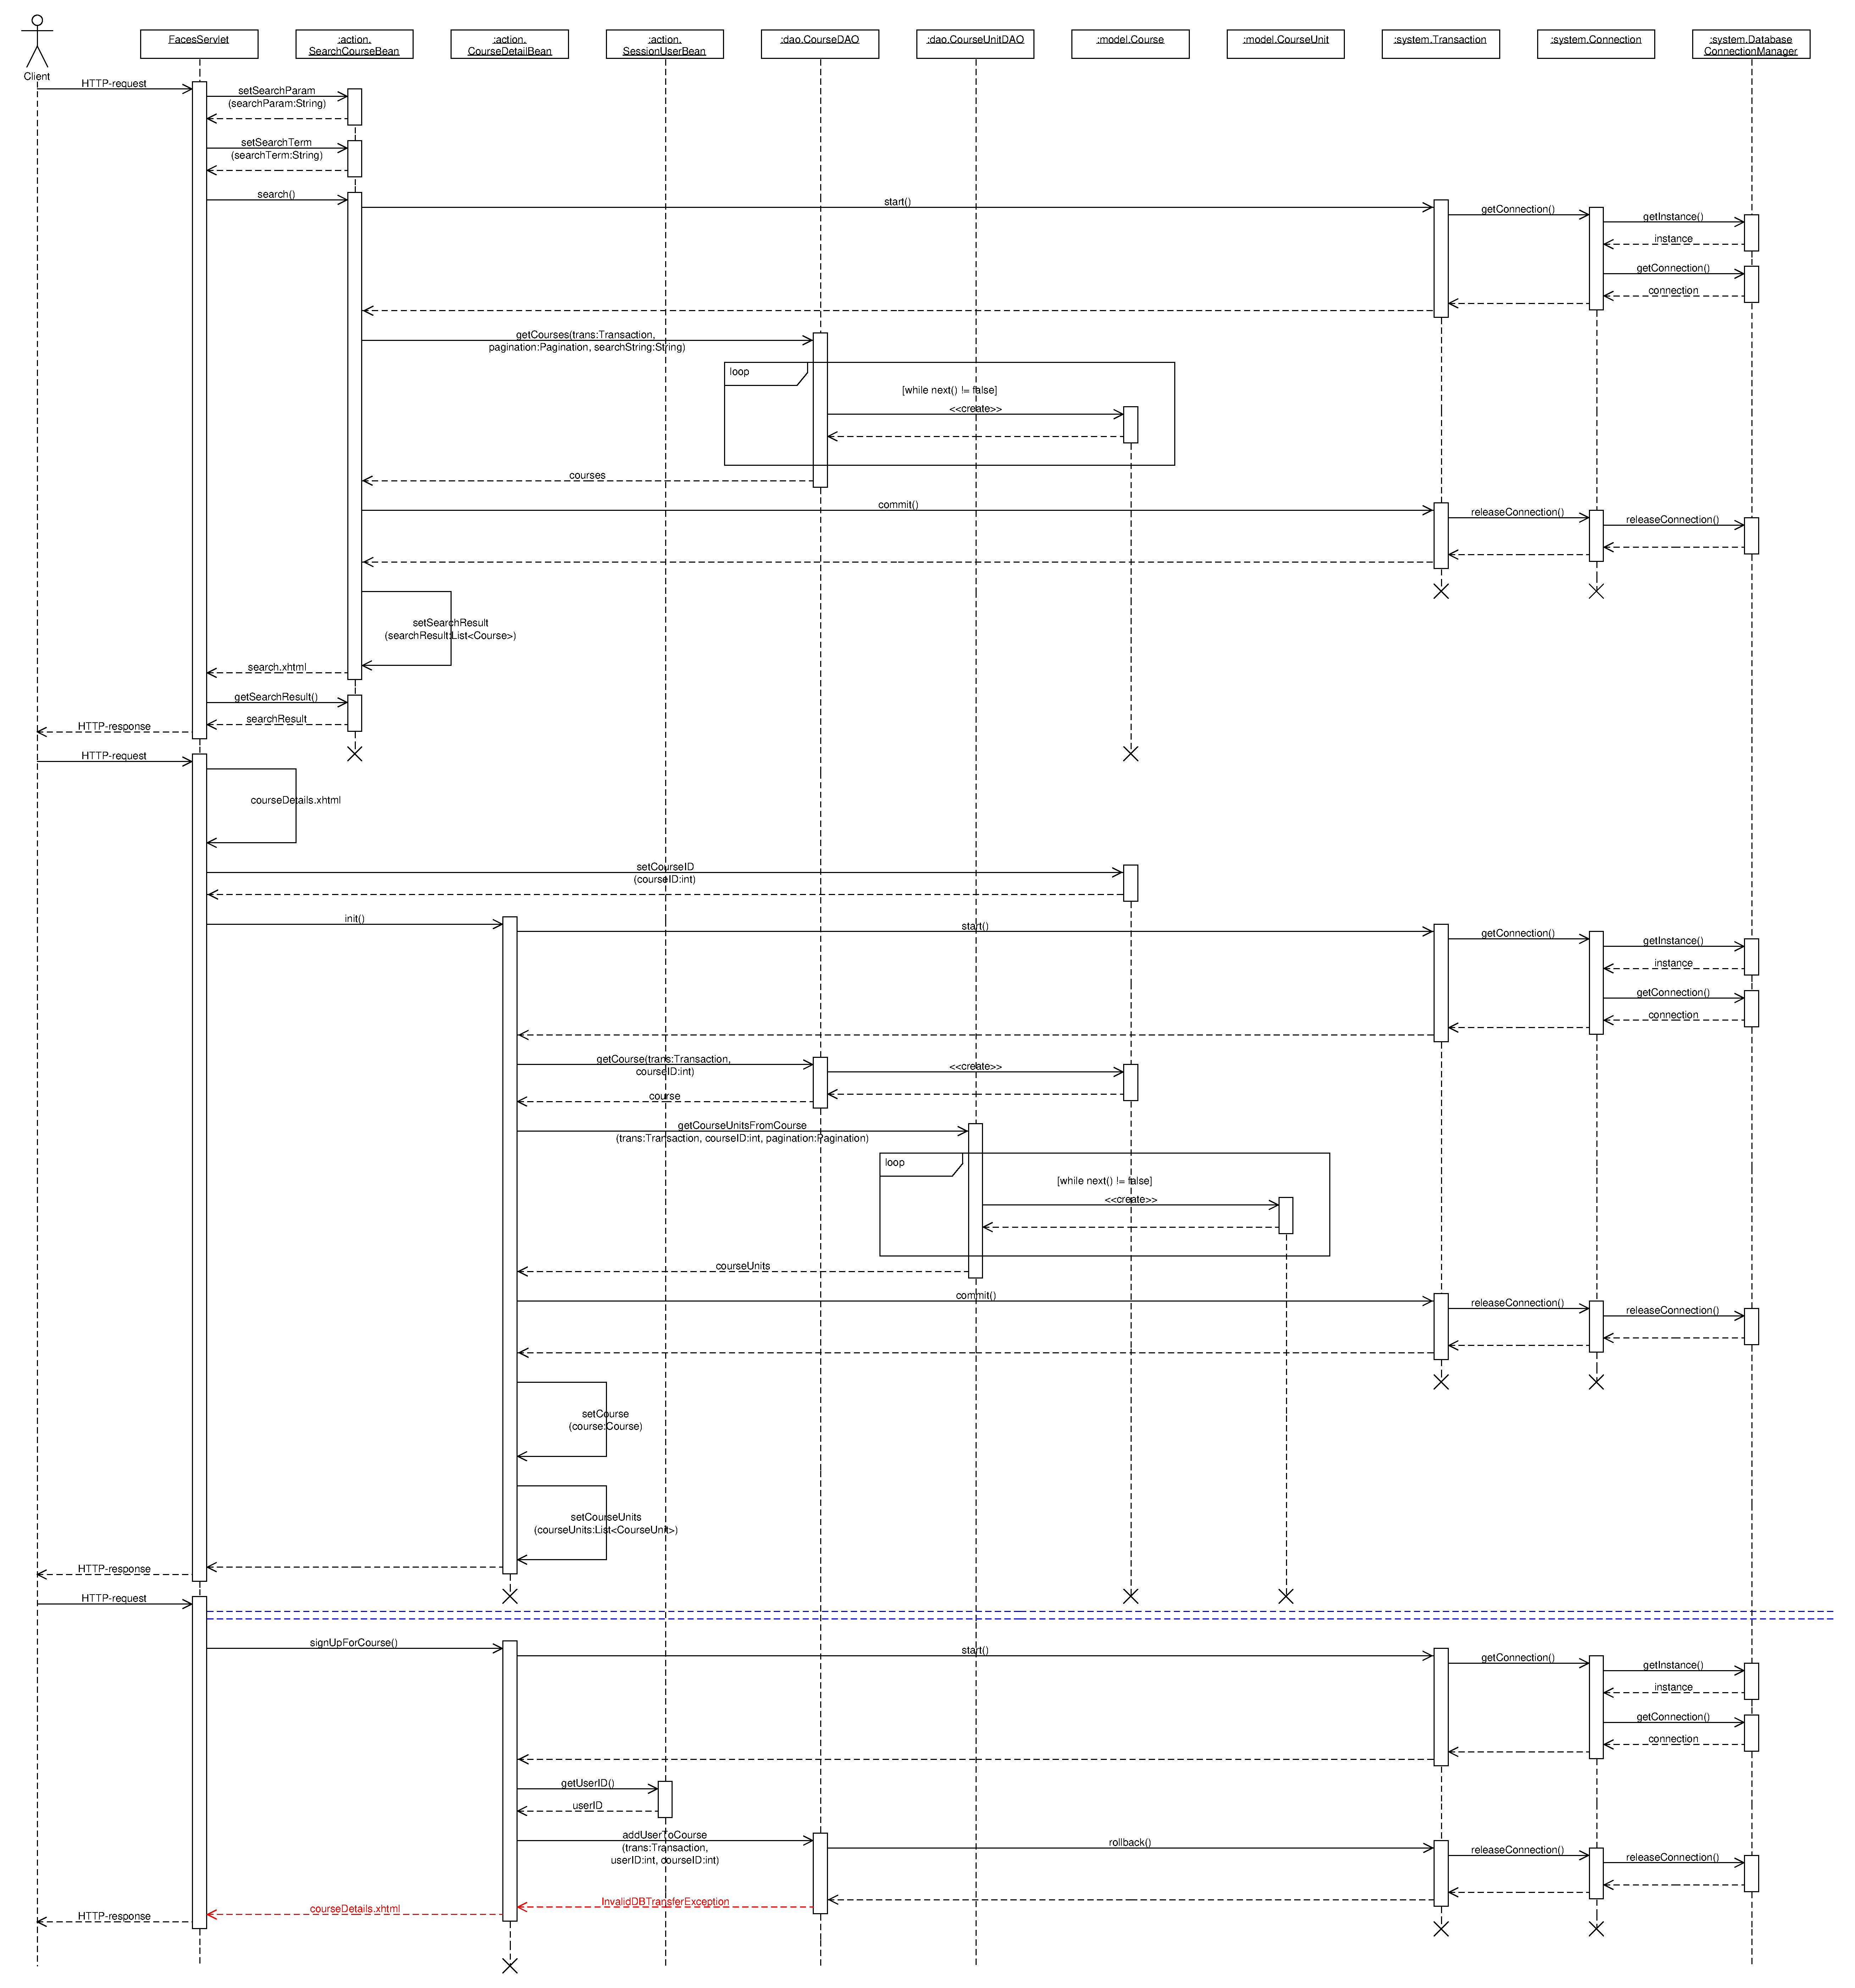
\includegraphics[scale=0.205]{./Grafiken/Sequenzdiagramm-Kursanmeldung.pdf}




\chapter{Security}
\begin{tiny}
	SeSc
\end{tiny}

\section{XSS(Cross-Site-Scripting), Javascript-Injection}
\subsection{Beschreibung}
Hierbei handelt es sich um eine Art HTML-Injection, die Auftritt wenn eine Webanwendung Daten von einem Nutzer annimmt und sie dann ohne zu prüfen an einen anderen Browser weitersendet. Damit können Angreifer auch Skripte auf den Browser eines anderen senden und Malware ausführen.
\subsection{Maßnahme}
JSF bietet bereits eine Gegenmaßnahme, indem bei allen Eingabefeldern das Attribute \textbf{escaped} auf \textbf{true} gestellt ist.

\section{SQL Injection}
\subsection{Beschreibung}
SQL Injection sind möglich wenn Daten, wie Benutzereingaben, in den SQL-Interpreter gelangen. Diese könnten Zeichen enthalten die eine Sonderfunktion für den SQL-Interpreter besitzen (z.B. Anführungszeichen, Backslash usw.) und damit Einfluss von außen auf die Datenbank ermöglichen. 
\subsection{Maßnahme}
Um diesen Vorgang zu verhindern, wird vom System der Befehl prepared Statement hergenommen. Damit werden die Daten als Parameter an einen bereits kompilierten Befehl übergeben und nicht interpretiert. Somit ist eine SQL Injection nicht möglich.


\section{Cross-site request forgery}
\subsection{Beschreibung}
Das Opfer muss an der Webanwendung bereits angemeldet sein und bekommt vom Angreifer einen HTTP-Request untergeschoben. Der Request ist so konzipiert, dass bei seinem Aufruf die Webanwendung, auf Opferseite, die gewünschte Aktion des Angreifers ausführt.
\subsection{Maßnahme}
Als Gegenmaßnahme wird das modifizieren von Inhalten durch GET-Requests nicht erlaubt und die HTTP-Referrer Header werden darauf geprüft ob die Anfrage von einer Seite des Systems kommt.


\section{Insecure Direct Object Reference}
\subsection{Beschreibung}
Hierbei wird versucht auf Daten zuzugreifen die dem Benutzer nicht zur Verfügung stehen.
\subsection{Maßnahme}
Bei jeder Anfrage wird überprüft ob der Benutzer, der die Anfrage gestellt hat, Zugriff auf die Daten haben darf.


\section{Session fixation}
\subsection{Beschreibung}
Der Angreifer versucht hier dem Opfer eine gültige, ihm vom System zugewiesene, Session-ID unterzuschieben. Wenn sich das Opfer jetzt einloggt und das System als Basis die ihm zugeschobene Session-ID benutzt, bekommt auch der Angreifer Zugriff auf das System da er sich ab diesen Zeitpunkt als Opfer ausgeben kann.
\subsection{Maßnahme}
Bei jedem Login wird dem Benutzer eine neue Session zugewiesen. Es wird außerdem sichergestellt, dass eine Session nicht unbegrenzt aktiv ist. Nach einer gewissen Zeit oder durch den Logout des Benutzers wird die Session mithilfe von invalidateSession zerstört.
\end{document}